% ─────────────────────────────────────────────────────────────────────────
% TWIN-LOCATION NOTICE. This file is one of the shared homes for the same
% results; edit every listed home or the drift checker fails.
%   Standalone paper : docs/harbor-research/tex/paper4.tex (S1-S9)
%   Chapter          : website-v2/public/whitepaper/sealed-harbor.tex (this
%                       file; the four-pillar assurance argument -- Pillars
%                       I, III, IV; Pillar II restates swk's R5)
%   Index ids        : R9, R10, R11
%   Check            : python3 scripts/harbor-research/check_library_index.py
%                      python3 scripts/harbor-research/check_propagated_corrections.py
%                      python3 scripts/harbor-research/check_citations.py
%   System document  : docs/harbor-research/LIBRARY-SYSTEM.md
% ─────────────────────────────────────────────────────────────────────────
\documentclass[11pt,a4paper]{article}

% ─── Packages ──────────────────────────────────────────────────────────────────
\usepackage[utf8]{inputenc}
\usepackage[T1]{fontenc}
\usepackage{lmodern}
\usepackage{microtype}
\usepackage{geometry}
\usepackage{amsmath,amssymb,amsthm}
\usepackage{listings}
\usepackage{xcolor}
\usepackage{booktabs}
\usepackage{tabularx}
\usepackage{graphicx}
\usepackage{fancyhdr}
\usepackage{tikz}
\usetikzlibrary{arrows.meta,positioning,fit,backgrounds,calc,shapes.geometric,shapes.symbols,decorations.pathmorphing,decorations.pathreplacing}
\usepackage{pgfplots}
\pgfplotsset{compat=1.18}
\usepackage{float}
\usepackage{caption}
\usepackage{enumitem}
\usepackage[backref=page]{hyperref}
\captionsetup{font=small,labelfont=bf}

% ─── Geometry ──────────────────────────────────────────────────────────────────
\geometry{margin=2.5cm}

% ─── Colors ───────────────────────────────────────────────────────────────────
\definecolor{codebg}{RGB}{248,248,248}
\definecolor{codeframe}{RGB}{200,200,200}
\definecolor{darkgreen}{HTML}{00564C}
\definecolor{darkblue}{HTML}{003FB8}
\definecolor{accent}{HTML}{00564C}
\definecolor{hhsand}{HTML}{E9DCC4}
\definecolor{hhsanddeep}{HTML}{D8C7A6}
\definecolor{hhebony}{HTML}{121212}
\definecolor{hhink}{HTML}{1B1712}
\definecolor{hhcobalt}{HTML}{003FB8}
\definecolor{hhamber}{HTML}{6B4500}
\definecolor{hhteal}{HTML}{00564C}
\definecolor{hhpaper}{HTML}{FBF7EF}
\definecolor{hhgray}{HTML}{5C5650}
% The Book's semantic color system: palette v2, light values. One hue, one meaning.
% Source of record for every hex: website-v2/src/styles/tokens.semantic.css (light
% theme); website-v2/scripts/check-figure-palette.mjs fails the build if this file
% and the tokens disagree. Twin copy under whitepaper/figures/ (byte-identical).
%
% Separation: contrast says an ink is READABLE on the cream; it says nothing about
% whether two inks are TELLABLE APART, and until now only the first was checked.
% check-figure-palette-separation.mjs measures all 21 pairs in OKLab with protanopia
% and deuteranopia simulated. indigo and violet are re-stepped (deeper, on their own
% hues, both gaining contrast) because they were the pairs with room: cobalt/indigo
% was dE 9.1 and is 15.1; cobalt/violet collapsed to 4.8 under protanopia and is 8.6.
% Three pairs CANNOT be fixed -- teal/health, gold/health and teal/gold have ceilings
% of 12.2, 13.9 and 14.3 against a floor of 15, because sRGB has no chroma to spend
% on the 112-182 degree arc this dark. Only ONE of gold, health and teal may carry a
% series by colour alone; the others need a label, a gap, or a texture.
%
% Discipline: story colors are accents (rules, fills, marks, display text); body
% pages stay cream and ink. Amber is stripes, dots, and display only, never small
% text (3.71:1 on cream). Violet and gold are AA as text; use them at display size
% or on rules and fills. Line weights: 1px texture, 1.5px linework, 2px enclosure.
\definecolor{pdcobalt}{HTML}{003FB8}      % kernel / truth            --brand-primary
\definecolor{pdteal}{HTML}{006B5F}        % legibility                --brand-accent
\definecolor{pdhealth}{HTML}{1F7A4D}      % ready / coordinated       --story-health
\definecolor{pdindigo}{HTML}{312865}      % protocol / federation     --story-indigo
\definecolor{pdviolet}{HTML}{822586}      % identity / continuity     --story-violet
\definecolor{pdrust}{HTML}{7A4514}        % reputation / trust earned --story-rust
\definecolor{pdgold}{HTML}{666A00}        % economy / value           --story-gold
\definecolor{pderror}{HTML}{BF2F2F}       % breach / correction       --status-error
\definecolor{pdamber}{HTML}{A66F00}       % warning (display only)    --status-warning
\definecolor{pdlime}{HTML}{CAD900}        % highlight fill, ink text  --chart-yellow
\definecolor{pdink}{HTML}{121212}         % ink                       --text-primary
\definecolor{pdinkmuted}{HTML}{403B34}    % links, secondary text     --text-secondary
\definecolor{pdcream}{HTML}{F2EEE6}       % page ground               --surface-base
\definecolor{pdcreamraised}{HTML}{F7F3EB} % panels                    --surface-raised
\definecolor{pdcreamstrong}{HTML}{E9E2D5} % inset wells               --surface-strong
% Print inks for the Swiss edition of the Book (SWISS-BRIEF, B); print only.
\definecolor{pdswissblue}{HTML}{001489}
\definecolor{pdswissviolet}{HTML}{582C83}
\definecolor{pdswissred}{HTML}{DA291C}
% And the maritime edition's fourth ink: antique gold, the trim of the engraved
% plates carried onto the page (opener rules, part-title ornament, fillets round
% framed matter). Flat stand-in for a metallic pass; print only.
\definecolor{pdmaritimegold}{HTML}{805A14}

\newcommand{\pdchapterprefix}{sealed}% this chapter's key in whitepaper/textbook.json
% GENERATED FILE. Do not edit by hand.
% Source of record: whitepaper/textbook.json (chapter order, numbers, parts, edition).
% Regenerate both committed copies: node scripts/generate-mega-whitepaper.mjs --sync-shared
% Drift check (CI): node --test scripts/generate-mega-whitepaper.test.mjs
% Twin copies: whitepaper/figures/pd-textbook-map.tex and
%              website-v2/public/whitepaper/figures/pd-textbook-map.tex (byte-identical).
%
% Every standalone chapter preamble defines \pdchapterprefix before inputting
% this file; the Book redefines it at every \pdchapter. Everything else derives.

\providecommand{\pdeditiontitle}{The Harbor, the Person, and the Economy}
\providecommand{\pdeditionsubtitle}{A textbook of accountable autonomous work}
\providecommand{\pdeditionversion}{4.0 (Textbook Edition)}
\providecommand{\pdeditiondate}{September 2026}
\providecommand{\pdeditionclaim}{Autonomy scales only when authority, evidence, and consequence remain coupled at every effect boundary.}
\providecommand{\pdbooktitle}{\emph{\pdeditiontitle}}
\providecommand{\pdchaptercount}{8}
\providecommand{\pdchaptercountword}{eight}
\providecommand{\pdpartcount}{4}
\providecommand{\pdchapterprefix}{none}
\expandafter\providecommand\csname pdchapternumberofnone\endcsname{0}
\expandafter\providecommand\csname pdchaptertitleofnone\endcsname{\pdeditiontitle}
\expandafter\providecommand\csname pdchaptercolorofnone\endcsname{pdcobalt}
\expandafter\providecommand\csname pdchapternumberofswk\endcsname{1}
\expandafter\providecommand\csname pdchaptertitleofswk\endcsname{The Single-Writer Kernel}
\expandafter\providecommand\csname pdchaptercolorofswk\endcsname{pdcobalt}
\expandafter\providecommand\csname pdchapterformerofswk\endcsname{II}
\expandafter\providecommand\csname pdchapterpartindexofswk\endcsname{1}
\expandafter\providecommand\csname pdchapterpartlabelofswk\endcsname{Part I \textperiodcentered\ Ground Truth}
\expandafter\providecommand\csname pdchapterquestionofswk\endcsname{Where can a rule be made real?}
\expandafter\providecommand\csname pdchapteronelineofswk\endcsname{One writer, one durable file, decides what is true so nothing above it has to guess.}
\expandafter\providecommand\csname pdchapterepigraphofswk\endcsname{A distributed system is one in which the failure of a computer you didn't even know existed can render your own computer unusable.}
\expandafter\providecommand\csname pdchapterepigraphsourceofswk\endcsname{Leslie Lamport, message to a DEC SRC bulletin board, 28 May 1987}
\expandafter\providecommand\csname pdchapternumberofanchor\endcsname{2}
\expandafter\providecommand\csname pdchaptertitleofanchor\endcsname{The Anchor Protocol}
\expandafter\providecommand\csname pdchaptercolorofanchor\endcsname{pdcobalt}
\expandafter\providecommand\csname pdchapterformerofanchor\endcsname{V}
\expandafter\providecommand\csname pdchapterpartindexofanchor\endcsname{1}
\expandafter\providecommand\csname pdchapterpartlabelofanchor\endcsname{Part I \textperiodcentered\ Ground Truth}
\expandafter\providecommand\csname pdchapterquestionofanchor\endcsname{How may authority travel without silently growing?}
\expandafter\providecommand\csname pdchapteronelineofanchor\endcsname{Delegated capability only narrows: every child is a subset of its parent, at every hop, and the verifier checks the whole chain.}
\expandafter\providecommand\csname pdchapterepigraphofanchor\endcsname{Every program and every user of the system should operate using the least set of privileges necessary to complete the job.}
\expandafter\providecommand\csname pdchapterepigraphsourceofanchor\endcsname{Jerome Saltzer and Michael Schroeder, The Protection of Information in Computer Systems, 1975}
\expandafter\providecommand\csname pdchapternumberofsealed\endcsname{3}
\expandafter\providecommand\csname pdchaptertitleofsealed\endcsname{The Sealed Harbor}
\expandafter\providecommand\csname pdchaptercolorofsealed\endcsname{pdcobalt}
\expandafter\providecommand\csname pdchapterformerofsealed\endcsname{}
\expandafter\providecommand\csname pdchapterpartindexofsealed\endcsname{1}
\expandafter\providecommand\csname pdchapterpartlabelofsealed\endcsname{Part I \textperiodcentered\ Ground Truth}
\expandafter\providecommand\csname pdchapterquestionofsealed\endcsname{What can a sealed agent leak, and how would we know?}
\expandafter\providecommand\csname pdchapteronelineofsealed\endcsname{A work order runs in a room with two fences and two gates, the only thing that leaves is what the slot lets out, and the budget of what can leak is a ledger that conserves.}
\expandafter\providecommand\csname pdchapterepigraphofsealed\endcsname{Whereof one cannot speak, thereof one must be silent.}
\expandafter\providecommand\csname pdchapterepigraphsourceofsealed\endcsname{Ludwig Wittgenstein, Tractatus Logico-Philosophicus, proposition 7, 1921 (Ogden translation, 1922)}
\expandafter\providecommand\csname pdchapternumberofls\endcsname{4}
\expandafter\providecommand\csname pdchaptertitleofls\endcsname{The Legible Swarm}
\expandafter\providecommand\csname pdchaptercolorofls\endcsname{pdteal}
\expandafter\providecommand\csname pdchapterformerofls\endcsname{I}
\expandafter\providecommand\csname pdchapterpartindexofls\endcsname{2}
\expandafter\providecommand\csname pdchapterpartlabelofls\endcsname{Part II \textperiodcentered\ The Cost of Seeing}
\expandafter\providecommand\csname pdchapterquestionofls\endcsname{What must remain visible, and what does seeing cost?}
\expandafter\providecommand\csname pdchapteronelineofls\endcsname{The operator's problem is blindness, not collision; supervision has an information cost you can price in bits.}
\expandafter\providecommand\csname pdchapterepigraphofls\endcsname{Certain forms of knowledge and control require a narrowing of vision. The great advantage of such tunnel vision is that it brings into sharp focus certain limited aspects of an otherwise far more complex and unwieldy reality.}
\expandafter\providecommand\csname pdchapterepigraphsourceofls\endcsname{James C. Scott, Seeing Like a State, 1998}
\expandafter\providecommand\csname pdchapternumberofstp\endcsname{5}
\expandafter\providecommand\csname pdchaptertitleofstp\endcsname{From Spawn to Person}
\expandafter\providecommand\csname pdchaptercolorofstp\endcsname{pdviolet}
\expandafter\providecommand\csname pdchapterformerofstp\endcsname{III}
\expandafter\providecommand\csname pdchapterpartindexofstp\endcsname{3}
\expandafter\providecommand\csname pdchapterpartlabelofstp\endcsname{Part III \textperiodcentered\ What Survives the Restart}
\expandafter\providecommand\csname pdchapterquestionofstp\endcsname{What remains long enough to owe anything?}
\expandafter\providecommand\csname pdchapteronelineofstp\endcsname{Continuity turns an anonymous spawn into a ledger position with a witnessed record; reputation is what that record is worth.}
\expandafter\providecommand\csname pdchapterepigraphofstp\endcsname{Person, as I take it, is the name for this self. It is a forensic term, appropriating actions and their merit; and so belongs only to intelligent agents, capable of a law, and happiness, and misery.}
\expandafter\providecommand\csname pdchapterepigraphsourceofstp\endcsname{John Locke, An Essay Concerning Human Understanding, II.xxvii.26, 1690}
\expandafter\providecommand\csname pdchapternumberofhe\endcsname{6}
\expandafter\providecommand\csname pdchaptertitleofhe\endcsname{The Harbor Economy}
\expandafter\providecommand\csname pdchaptercolorofhe\endcsname{pdgold}
\expandafter\providecommand\csname pdchapterformerofhe\endcsname{IV}
\expandafter\providecommand\csname pdchapterpartindexofhe\endcsname{4}
\expandafter\providecommand\csname pdchapterpartlabelofhe\endcsname{Part IV \textperiodcentered\ Trade Between Strangers}
\expandafter\providecommand\csname pdchapterquestionofhe\endcsname{What makes cooperation rational without making loss unbounded?}
\expandafter\providecommand\csname pdchapteronelineofhe\endcsname{Once records cannot be minted, trust can be rented between operators who never met: a three-sided market on one conserving ledger.}
\expandafter\providecommand\csname pdchapterepigraphofhe\endcsname{Virtually every commercial transaction has within itself an element of trust, certainly any transaction conducted over a period of time.}
\expandafter\providecommand\csname pdchapterepigraphsourceofhe\endcsname{Kenneth J. Arrow, Gifts and Exchanges, 1972}
\expandafter\providecommand\csname pdchapternumberofbonded\endcsname{7}
\expandafter\providecommand\csname pdchaptertitleofbonded\endcsname{The Bonded Commons}
\expandafter\providecommand\csname pdchaptercolorofbonded\endcsname{pdgold}
\expandafter\providecommand\csname pdchapterformerofbonded\endcsname{VI}
\expandafter\providecommand\csname pdchapterpartindexofbonded\endcsname{4}
\expandafter\providecommand\csname pdchapterpartlabelofbonded\endcsname{Part IV \textperiodcentered\ Trade Between Strangers}
\expandafter\providecommand\csname pdchapterquestionofbonded\endcsname{Who may decide, on what evidence, with what consequence?}
\expandafter\providecommand\csname pdchapteronelineofbonded\endcsname{Bonds, witnesses, audits and appeals turn residual uncertainty into an institution; the ledger's conservation law is mechanically checked.}
\expandafter\providecommand\csname pdchapterepigraphofbonded\endcsname{If men were angels, no government would be necessary. If angels were to govern men, neither external nor internal controls on government would be necessary.}
\expandafter\providecommand\csname pdchapterepigraphsourceofbonded\endcsname{James Madison, Federalist No. 51, 1788}
\expandafter\providecommand\csname pdchapternumberoffh\endcsname{8}
\expandafter\providecommand\csname pdchaptertitleoffh\endcsname{The Federated Harbor}
\expandafter\providecommand\csname pdchaptercoloroffh\endcsname{pdgold}
\expandafter\providecommand\csname pdchapterformeroffh\endcsname{VII}
\expandafter\providecommand\csname pdchapterpartindexoffh\endcsname{4}
\expandafter\providecommand\csname pdchapterpartlabeloffh\endcsname{Part IV \textperiodcentered\ Trade Between Strangers}
\expandafter\providecommand\csname pdchapterquestionoffh\endcsname{What can cross a trust boundary without moving the authority itself?}
\expandafter\providecommand\csname pdchapteronelineoffh\endcsname{Mutually distrustful machines relay evidence, not sovereignty: what may gossip, what needs an authority point, and how a grant crosses a boundary.}
\expandafter\providecommand\csname pdchapterepigraphoffh\endcsname{Good fences make good neighbours.}
\expandafter\providecommand\csname pdchapterepigraphsourceoffh\endcsname{Robert Frost, Mending Wall, 1914}
\providecommand{\pdchapternumber}{\csname pdchapternumberof\pdchapterprefix\endcsname}
\providecommand{\pdchaptertitle}{\csname pdchaptertitleof\pdchapterprefix\endcsname}
\providecommand{\pdchaptercolor}{\csname pdchaptercolorof\pdchapterprefix\endcsname}
\providecommand{\pdchapterpartindex}{\csname pdchapterpartindexof\pdchapterprefix\endcsname}
\providecommand{\pdchapterpartlabel}{\csname pdchapterpartlabelof\pdchapterprefix\endcsname}
\providecommand{\pdchapterquestion}{\csname pdchapterquestionof\pdchapterprefix\endcsname}
\providecommand{\pdchapteroneline}{\csname pdchapteronelineof\pdchapterprefix\endcsname}
\providecommand{\pdchapterepigraph}{\csname pdchapterepigraphof\pdchapterprefix\endcsname}
\providecommand{\pdchapterepigraphsource}{\csname pdchapterepigraphsourceof\pdchapterprefix\endcsname}

% Parts, for the weighted four-hue rule: numeral, hue, the label that ends the
% part (the next part, or the appendices), and the chapter count used as the
% weight until page references exist. \pdweightrule (Book preamble) consumes it.
\providecommand{\pdfirstpartnumeral}{I}
\providecommand{\pdweightsegmentslist}{%
  \pdweightsegment{I}{pdcobalt}{part:II}{3}%
  \pdweightsegment{II}{pdteal}{part:III}{1}%
  \pdweightsegment{III}{pdviolet}{part:IV}{1}%
  \pdweightsegment{IV}{pdgold}{book:appendices}{3}%
}
\expandafter\providecommand\csname pdpartindexofI\endcsname{1}
\expandafter\providecommand\csname pdpartindexofII\endcsname{2}
\expandafter\providecommand\csname pdpartindexofIII\endcsname{3}
\expandafter\providecommand\csname pdpartindexofIV\endcsname{4}
\expandafter\providecommand\csname pdparttitleofI\endcsname{Ground Truth}
\expandafter\providecommand\csname pdparttitleofII\endcsname{The Cost of Seeing}
\expandafter\providecommand\csname pdparttitleofIII\endcsname{What Survives the Restart}
\expandafter\providecommand\csname pdparttitleofIV\endcsname{Trade Between Strangers}

% Locator map: every part and chapter of the Book, the current chapter marked.
% \pdchaplink is provided by figures/pd-hyperlinks.tex (a live link inside the
% Book, plain text in a standalone chapter).
\providecommand{\pdmapchapter}[3]{%
  \ifnum#1=\pdchapternumber\relax
    \textbf{\pdchaplink{#2}{#1.~#3}}~\textnormal{(this chapter)}%
  \else
    \pdchaplink{#2}{#1.~#3}%
  \fi}
\providecommand{\pdtextbookmap}{%
  \begin{tabular}{@{}l@{\quad}p{\dimexpr\linewidth-12em\relax}@{}}
  \textsc{\textbf{Part I}}\ Ground Truth & \raggedright \pdmapchapter{1}{swk}{The Single-Writer Kernel} \textperiodcentered\ \pdmapchapter{2}{anchor}{The Anchor Protocol} \textperiodcentered\ \pdmapchapter{3}{sealed}{The Sealed Harbor}\tabularnewline[2pt]
  \textsc{\textbf{Part II}}\ The Cost of Seeing & \raggedright \pdmapchapter{4}{ls}{The Legible Swarm}\tabularnewline[2pt]
  \textsc{\textbf{Part III}}\ What Survives the Restart & \raggedright \pdmapchapter{5}{stp}{From Spawn to Person}\tabularnewline[2pt]
  \textsc{\textbf{Part IV}}\ Trade Between Strangers & \raggedright \pdmapchapter{6}{he}{The Harbor Economy} \textperiodcentered\ \pdmapchapter{7}{bonded}{The Bonded Commons} \textperiodcentered\ \pdmapchapter{8}{fh}{The Federated Harbor}\tabularnewline[2pt]
  \end{tabular}}

% Shared pedagogic apparatus for the Book and every standalone chapter: boxed
% claims, honest boundaries, worked examples, retrieval prompts, numbered
% exercises, and their deferred solutions.
% Twin copy under whitepaper/figures/ (byte-identical; checked by
% scripts/generate-mega-whitepaper.test.mjs).
%
% \input this immediately after figures/pd-textbook-map (so \pdchapterprefix
% and \pdchapternumber already resolve) and before figures/pd-hyperlinks.
%
% Page grammar (Wave 12): a content kind is signalled by typography and the
% margin, never by a tinted rectangle. Claims: a hairline above, a small-caps
% run-in head, a short hairline below. Worked examples: two hairlines and an
% italic head. Boundaries: a plain ink bar at the left, no fill. Recitation:
% margin prompts in the Book, a compact list in a standalone chapter.
% Exercises: a numbered hanging paragraph with kind and stars in small caps,
% the solution page in the margin. Nothing here paints a background.
%
% \ifpdmargincolumn is false by default (standalone A4 chapters have no margin
% column); the Book's preamble sets \pdmargincolumntrue after its geometry.
% mdframed is used only for the bars (leftline) and hairlines (top/bottom),
% with the DEFAULT frame method -- never framemethod=tikz.
%
% Key-value parsing for \pdexercise uses pgfkeys: pgf ships as part of tikz,
% which every preamble already loads, so this adds no new dependency (keyval
% would have meant one). The closed kind/rating vocabularies are enforced with
% the LaTeX kernel's own \in@/\ifin@ comma-list test -- always available,
% no package of its own -- wrapped in an \edef that expands both sides first:
% \in@ does not expand its own arguments, so hunting for a *macro* (rather
% than literal text) requires pre-expanding it, or every kind reads as absent.
\makeatletter
\@ifpackageloaded{mdframed}{}{\usepackage{mdframed}}
\@ifpackageloaded{answers}{}{\usepackage{answers}}
\@ifpackageloaded{marginnote}{}{\usepackage{marginnote}}
\@ifpackageloaded{environ}{}{\usepackage{environ}}
\@ifpackageloaded{etoolbox}{}{\usepackage{etoolbox}}
\@ifpackageloaded{listings}{}{\usepackage{listings}}
\@ifpackageloaded{caption}{}{\usepackage{caption}}
\@ifpackageloaded{tcolorbox}{}{\usepackage[skins,breakable,listings]{tcolorbox}}

% ---------------------------------------------------------------------------
% Shared helpers: the margin-column switch, the margin head, the margin glyph.
% ---------------------------------------------------------------------------
% The Book defines \pdcurrentchaptercolor (per part) AFTER this file; a
% standalone chapter never does. Resolve it lazily, falling back to cobalt.
\newcommand{\pd@chaptercolor}{\ifdefined\pdcurrentchaptercolor\pdcurrentchaptercolor\else pdcobalt\fi}
% The eight standalone chapter PDFs this false branch exists for are retired
% as of this change (the chapters no longer build or publish an A4 edition of
% themselves). Every \ifpdmargincolumn false branch below is now dead weight
% kept alive only by the chapters' .tex sources still being independently
% compilable; do NOT delete it in this change -- the margin apparatus work is
% in flight on another branch and this would collide with it. Removing the
% false branch (and, eventually, the conditional itself) is that wave's job.
\newif\ifpdmargincolumn
\pdmargincolumnfalse
% The Book overrides this with an unnumbered, baseline-aligned margin aside.
% Keep chapter sources independently compilable without duplicating prose.
\providecommand{\pdsourceaside}[1]{\footnote{#1}}
% An intentional body boundary: flush pending figures before a new margin
% discussion. The generator strips legacy literal chapter-opening breaks,
% but preserves this explicit editorial instruction. Never use it in frames.
\newcommand{\pdmarginpagebreak}{\clearpage}
\renewcommand*{\marginfont}{\footnotesize\raggedright\color{pdinkmuted}}
% A small-caps head: set in the margin when the Book has a margin column,
% otherwise run in at the start of the paragraph.
% A head stays a \marginnote, and the reason is worth keeping. It was set as
% a \marginpar for one build (2026-09-08), so the page builder would keep the
% Recall block clear of it, and the build died with "Float(s) lost" at the end
% of chapter 1. \ifinner is true inside a minipage or mdframed only BETWEEN
% paragraphs; the moment a paragraph starts it is ordinary horizontal mode,
% \ifinner is false, and a \marginpar issued there -- a \keyidea inside a
% pdexample -- has no page to be shipped to. The heads are one line each and
% are never what runs into something; the Recall block was, and it is now a
% \marginpar issued in vertical mode, where the test is honest.
% Each head records the page and the page-height at which it was issued, so a
% Recall block raised later on the same page can stop short of it. A head is
% issued at the start of its paragraph, where \pagetotal is the page above the
% paragraph -- the head's own position, to within a line.
% Margin occupancy is tracked both ways. A head records where it was issued
% so a Recall block raised later on the page stops short of it; a Recall block
% records where its foot came to rest so a head issued later on the same page
% (the next section's first Key idea) steps down below it instead of printing
% inside it. \pagetotal at a head lags by the current paragraph, which puts
% every error on the safe side: the block is capped a little low, the head
% steps a little far.
\def\pd@lastheadpage{0}\newlength{\pd@lastheadbottom}
\def\pd@blockpage{0}\newlength{\pd@blockbottom}\newlength{\pd@headshift}
\newsavebox{\pd@headbox}\newsavebox{\pd@ptrbox}\newsavebox{\pd@sidebox}
% Run the page builder so \pagetotal counts the paragraph that just ended.
% Without it \pagetotal is the page above the LAST paragraph the builder saw,
% which under-reads by however much prose has since been set -- and every
% device here decides where it may sit from that number. A Boundary head read
% a stale \pagetotal and recorded its foot a paragraph too high, and the Recall
% block that followed cleared that phantom and printed on the head itself
% (0.1 pt apart on p. 253 of the technical edition). \penalty\@M contributes
% without opening a breakpoint. Outer vertical mode only: inside a box the
% penalty lands on the box's own list and settles nothing.
\newcommand{\pd@settle}{\ifvmode\ifinner\else\penalty\@M\vskip\z@\fi\fi}
% ---------------------------------------------------------------------------
% Figure-band tracking, for vertical CENTERING of a margin device against the
% main-column figure it accompanies (2026-09). \pd@figtop/\pd@figbot/\pd@figpage
% are declared here but SET in the Book preamble's \pgfsys@typesetpicturebox
% hook (coordination-papers-mega-volume-preamble.tex), not by an
% \AtBeginEnvironment{figure}/\AtEndEnvironment{figure} pair on \pagetotal --
% that was the first attempt and it does not work: for a \begin{figure}[H]
% float, the `float' package defers inserting the box into the main vertical
% list past \end{figure} itself, so \pagetotal read there under-reads by the
% whole figure and \pd@figbot always came out equal to \pd@figtop (measured:
% every firing in the built Book). The pgf hook that already intercepts every
% TikZ picture on its way into the page knows the box's own \ht+\dp directly,
% which is exact regardless of page-builder timing, so that is where the span
% is recorded now. \pd@figpage guards against reading a stale span left over
% from a figure several pages back: \pd@placemargin only trusts the span when
% \pd@figpage still equals the numeric page counter. Only one span is kept -- the most
% recently drawn picture on this page -- which is deliberately the figure a
% margin device issued shortly afterward is almost always about; a page with
% two unrelated figures and one margin device between them is not a case this
% file has seen.
\newlength{\pd@figtop}\newlength{\pd@figbot}\def\pd@figpage{0}
% Does OFFSET (already sitting in \pd@blockoff) sit inside the room this page
% actually has for it, without moving? \pd@reqmin/\pd@reqmax are computed by
% \pd@marginbounds below, from exactly the three collision facts \pd@placemargin
% already knew about (page top, the last margin head, the last margin block) --
% this is a read of the same facts, not a new rule. A candidate that fits
% clean is preferred over one merely clamped INTO range, because a clamped
% value is a collision this page already had; a candidate the bounds do not
% touch is one that was never in anyone's way.
\newlength{\pd@reqmin}\newlength{\pd@reqmax}\newif\ifpd@havemax\newif\ifpd@fits
\newcommand{\pd@marginbounds}[1]{%
  \setlength{\pd@reqmin}{-\pagetotal}%
  \ifnum\pd@lastheadpage=\value{page}\relax
    \ifdim\pd@reqmin<\dimexpr\pd@lastheadbottom-\pagetotal\relax
      \setlength{\pd@reqmin}{\dimexpr\pd@lastheadbottom-\pagetotal\relax}\fi\fi
  \ifnum\pd@blockpage=\value{page}\relax
    \ifdim\pd@reqmin<\dimexpr\pd@blockbottom-\pagetotal+2pt\relax
      \setlength{\pd@reqmin}{\dimexpr\pd@blockbottom-\pagetotal+2pt\relax}\fi\fi
  \ifdim\pagegoal<\maxdimen
    \pd@havemaxtrue
    \setlength{\pd@reqmax}{\dimexpr\pagegoal-\pagetotal-\ht#1-\dp#1\relax}%
  \else\pd@havemaxfalse\fi}
\newcommand{\pd@tryoffset}{%
  \pd@fitstrue
  \ifdim\pd@blockoff<\pd@reqmin\pd@fitsfalse\fi
  \ifpd@fits\ifpd@havemax\ifdim\pd@blockoff>\pd@reqmax\pd@fitsfalse\fi\fi\fi}
\newcommand{\pd@marginhead}[1]{%
  \ifpdmargincolumn
    % Settle before the first \pagetotal read, unlike this macro's earlier
    % form. Every OTHER margin device in this file settles first (the
    % comment two macros up even says why: "\pagetotal is the page above
    % the LAST paragraph the builder saw"), but this one read \pagetotal
    % raw at the head's own issuing point and called the resulting slop
    % "to within a line" -- acceptable when a block follows a head closely,
    % not when many lines of prose come between them and a margin block
    % later clamps to \pd@lastheadbottom expecting it exact. Measured: a
    % \pdboundary head ("Where this stops") 14 lines above its section's
    % \end{pdrecitation}, recorded 2.35 pt short, so the Recall block's
    % clamp (aimed at a 3 pt gap under the head) landed 2.35 pt INSIDE it
    % instead -- built and measured overlapping, PDF p. 244.
    \pd@settle
    \setlength{\pd@headshift}{0pt}%
    \ifnum\pd@blockpage=\value{page}\relax
      \ifdim\pagetotal<\pd@blockbottom
        \setlength{\pd@headshift}{\dimexpr\pd@blockbottom-\pagetotal+3pt\relax}\fi
    \fi
    % And around the last HEAD on this page, which this macro recorded below
    % and then never read. Blocks stepped around heads, heads stepped around
    % blocks, and two heads walked straight through each other: a Pitfall head
    % printed 1.0 pt from a Recall head at the top of p. 306 of the maritime
    % edition, inside the 10.4 pt leading the collision check measures. The
    % rule is the same one \pd@placemargin already obeys three lines at a
    % time -- never above what is already in the column -- so it is applied
    % here in the same shape, after the block cap so whichever foot sits
    % lower wins.
    \ifnum\pd@lastheadpage=\value{page}\relax
      \ifdim\dimexpr\pagetotal+\pd@headshift\relax<\pd@lastheadbottom
        \setlength{\pd@headshift}{\dimexpr\pd@lastheadbottom-\pagetotal+3pt\relax}\fi
    \fi
    % A twin of the head, set at the margin's width and font, measured but
    % never shipped: a head of three or four words wraps to two lines there,
    % and a block raised later on the page has to clear the head's real foot.
    % Assuming one line put "RECALL" 0.1 pt under "WHERE THIS STOPS" in the
    % Swiss and technical editions, whose pagination differs from the
    % maritime edition's by a page.
    \sbox{\pd@headbox}{\begin{minipage}{\marginparwidth}\marginfont\scshape #1\end{minipage}}%
    \marginnote{\scshape #1}[\pd@headshift]%
    \xdef\pd@lastheadpage{\number\value{page}}%
    % +8pt, not +3pt: \pd@headbox measures the head's own text, but the
    % marginnote package sets every note's content behind a \strut (its
    % \marginfont\raggedrightmarginnote\strut...) whose height+depth come
    % from \marginfont's normal font metrics, not from \scshape "Where this
    % stops" alone -- the strut is measurably taller, so \ht+\dp here
    % under-reads the head's true rendered bottom. +3pt covered one 0.1pt
    % case (comment above); it did not cover this one -- built and measured
    % a Recall block clamped to +3pt still overlapping "Where this stops" by
    % 2.35 pt (PDF p. 244, pdboundary fourteen lines above its section's
    % \end{pdrecitation}). +8pt re-measured clear on that page and does not
    % reopen the "1.3 pt under" case the \newpage reservation above already
    % handles (a different mechanism -- a migrated page, not a short strut).
    \global\pd@lastheadbottom=\dimexpr\pagetotal+\pd@headshift
      +\ht\pd@headbox+\dp\pd@headbox+8pt\relax
  \else{\scshape\bfseries #1.}\enspace\fi}
% A small square in the chapter's hue, in the margin, marking a worked example
% so a reader flipping through finds every one.
\newlength{\pd@blockoff}
% Place a measured margin block so its LAST line sits on the line that issues
% it -- the block occupies the page above its anchor rather than hanging below
% it, which is what keeps a note issued near the foot on the paper at all.
% Three caps, in order: never above the page top; never above the last margin
% head on this page (measured to that head's own foot); never above the last
% block on this page. Then the block records where its foot came to rest, so a
% head issued later steps down below it. \pagetotal is the shared clock for all
% of this, which is why every device that can settles the page builder first.
% Every margin device goes through here, including the three the margin
% apparatus added (\pdcite, \pdprov, \pdprovedon): a device that places its
% own note without asking what is already in the column is how the Book got
% seven collisions and a portrait below the paper, and there are now several
% hundred short notes in the column where there were dozens.
% Place a margin block with its TOP on the issuing line rather than its foot.
% Same occupancy bookkeeping as \pd@placemargin -- it must, or a later block
% would be told the column is free where this one sits -- but it never raises,
% so it cannot leave the page above. Clamped both ways: the offset is never
% negative (nothing above the text block) and, where \pagegoal is a real
% dimension, never so large that the block's foot passes the bottom of the
% text block. \pagegoal is \maxdimen on an empty page, which is room for
% anything; a block already taller than its page is left alone rather than
% shoved, because moving it cannot make it fit.
\newlength{\pd@blockfloor}
\newcommand{\pd@placemargintop}[1]{%
  \setlength{\pd@blockoff}{0pt}%
  \ifnum\pd@lastheadpage=\value{page}\relax
    \ifdim\pd@blockoff<\dimexpr\pd@lastheadbottom-\pagetotal\relax
      \setlength{\pd@blockoff}{\dimexpr\pd@lastheadbottom-\pagetotal\relax}\fi
  \fi
  \ifnum\pd@blockpage=\value{page}\relax
    \ifdim\pd@blockoff<\dimexpr\pd@blockbottom-\pagetotal+2pt\relax
      \setlength{\pd@blockoff}{\dimexpr\pd@blockbottom-\pagetotal+2pt\relax}\fi
  \fi
  \ifdim\pd@blockoff<0pt \setlength{\pd@blockoff}{0pt}\fi
  % The floor the two caps above just established: whatever is already in the
  % column on this page ends here, and nothing may be placed above it.
  \setlength{\pd@blockfloor}{\pd@blockoff}%
  % Pull the block up if its foot would pass the bottom of the text block --
  % but never above that floor. Reducing the offset past it is how the
  % foot-anchored placement used to undo its own downward pushes: a clamp
  % applied last re-collides the block with the head or the note it was just
  % moved clear of, which is the defect this file's other comment records as
  % 132 collisions on one merge. A block too tall to satisfy both is left at
  % the floor and overruns the foot, where page_overflow.py's foot-intrusion
  % and off-the-paper checks will report it -- a visible, measured overrun is
  % worth more than a silent overlap.
  \ifdim\pagegoal<\maxdimen
    \ifdim\dimexpr\pagetotal+\pd@blockoff+\ht#1+\dp#1\relax>\pagegoal
      \setlength{\pd@blockoff}{\dimexpr\pagegoal-\pagetotal-\ht#1-\dp#1\relax}%
      \ifdim\pd@blockoff<\pd@blockfloor \setlength{\pd@blockoff}{\pd@blockfloor}\fi
    \fi
  \fi
  \marginnote{\usebox#1}[\pd@blockoff]%
  \xdef\pd@blockpage{\number\value{page}}%
  \global\pd@blockbottom=\dimexpr\pagetotal+\pd@blockoff+\ht#1+\dp#1\relax}

% Default placement is now CENTERED on the vertical span of the most recently
% closed figure on this page, not anchored to the line that issues the note --
% a Recall block or a gloss discussing a figure reads naturally beside its
% middle, not hanging off one edge. Center only WHEN IT FITS CLEAN: tried
% against \pd@marginbounds's read of the same three collision facts the old
% single anchor already obeyed (page top, the last margin head, the last
% margin block), with no clamping. A center that does not fit clean is not
% clamped into place -- clamping a center is neither center nor top nor
% bottom, it is just wherever the clamp landed, and the point of asking for an
% aligned center was to get one honestly or not at all. Top-of-figure is tried
% next, then bottom-of-figure; the first of the three that needs no clamp
% wins. If none does, this falls through unchanged to the pre-existing
% issuing-line anchor and its own clamps below -- the same fallback this file
% always had, now reached only when no figure-relative placement clears.
\newif\ifpd@figcentered
\newcommand{\pd@placemargin}[1]{%
  \pd@figcenteredfalse
  \ifnum\pd@figpage=\value{page}\relax\ifdim\pd@figbot>\z@
    \pd@marginbounds{#1}%
    \setlength{\pd@blockoff}{\dimexpr(\pd@figtop+\pd@figbot)/2-\pagetotal-(\ht#1+\dp#1)/2\relax}%
    \pd@tryoffset
    \ifpd@fits\pd@figcenteredtrue\else
      \setlength{\pd@blockoff}{\dimexpr\pd@figtop-\pagetotal\relax}%
      \pd@tryoffset
      \ifpd@fits\pd@figcenteredtrue\else
        \setlength{\pd@blockoff}{\dimexpr\pd@figbot-\pagetotal-\ht#1-\dp#1\relax}%
        \pd@tryoffset
        \ifpd@fits\pd@figcenteredtrue\fi
      \fi
    \fi
  \fi\fi
  \ifpd@figcentered
    \marginnote{\usebox#1}[\pd@blockoff]%
    \xdef\pd@blockpage{\number\value{page}}%
    \global\pd@blockbottom=\dimexpr\pagetotal+\pd@blockoff+\ht#1+\dp#1\relax
  \else
  \setlength{\pd@blockoff}{\dimexpr\baselineskip-\ht#1-\dp#1\relax}%
  % A note never starts below the line that issues it -- clamped here, BEFORE
  % the occupancy caps, not after. Clamping last undid every downward push:
  % two \pdcite calls in one paragraph read the same \pagetotal, so the second
  % was told to start below the first's foot and then clamped straight back
  % onto it (132 collisions on the merge, all of them pairs of citations on
  % one line). Below the anchor is exactly where a second note belongs.
  \ifdim\pd@blockoff>0pt \setlength{\pd@blockoff}{0pt}\fi
  \ifdim\pd@blockoff<-\pagetotal
    \setlength{\pd@blockoff}{-\pagetotal}%
    % Headroom at the column top, and the reason is the one hole left in the
    % occupancy model. Every cap below is keyed on the numeric page counter, which is the
    % page the device was ISSUED on -- and a head issued in the last line of
    % a page whose paragraph then breaks prints at the top of the NEXT page
    % while having recorded the page before. That is exactly the Recall-on-
    % Pitfall collision at the top of p. 306 of the maritime edition: the
    % Pitfall head began its paragraph at the foot of p. 305, migrated with
    % the break, and the Recall block clamped flush to p. 306's column top
    % and landed 1.0 pt from a head no cap could see. TeX cannot tell us the
    % shipout page here, so the fix is not a better cap but a reservation:
    % when the top clamp binds, leave two lines for whatever may have come
    % over the break. Two, not one, because a head of three or four words
    % wraps to two lines at the margin's width. Only when there is room --
    % \pagegoal is \maxdimen on an empty page, which is room enough for
    % anything, and a block already too tall for its page is left where the
    % clamp put it rather than pushed off the paper.
    \ifdim\dimexpr\pagetotal+\pd@blockoff+2\baselineskip+\ht#1+\dp#1\relax>\pagegoal
      \ifdim\dimexpr\pagetotal+\pd@blockoff+\baselineskip+\ht#1+\dp#1\relax>\pagegoal
      \else\setlength{\pd@blockoff}{\dimexpr\pd@blockoff+\baselineskip\relax}\fi
    \else\setlength{\pd@blockoff}{\dimexpr\pd@blockoff+2\baselineskip\relax}\fi
  \fi
  \ifnum\pd@lastheadpage=\value{page}\relax
    \ifdim\pd@blockoff<\dimexpr\pd@lastheadbottom-\pagetotal\relax
      \setlength{\pd@blockoff}{\dimexpr\pd@lastheadbottom-\pagetotal\relax}\fi
  \fi
  \ifnum\pd@blockpage=\value{page}\relax
    \ifdim\pd@blockoff<\dimexpr\pd@blockbottom-\pagetotal+2pt\relax
      \setlength{\pd@blockoff}{\dimexpr\pd@blockbottom-\pagetotal+2pt\relax}\fi
  \fi
  \marginnote{\usebox#1}[\pd@blockoff]%
  \xdef\pd@blockpage{\number\value{page}}%
  \global\pd@blockbottom=\dimexpr\pagetotal+\pd@blockoff+\ht#1+\dp#1\relax
  \fi}
% The same placement for a note the page can do without. A Recall block, a
% margin figure and a gloss carry content that is nowhere else, so they are
% always placed. A short-form citation, a provenance note and a discharge
% pointer are second copies: \pdcite has already emitted the \cite, so the
% work is in the text and in the bibliography whatever the margin does. There
% are several hundred of them and on a dense page the column has no room for
% one beside every line that cites -- arithmetic cannot make space that is not
% there. So when placing one would push its foot past the text block's foot,
% it is left out rather than printed over its neighbour or below the paper.
% Nothing is lost that a reader could otherwise have read.
\newcommand{\pd@placemarginopt}[1]{%
  \setlength{\pd@blockoff}{\dimexpr\baselineskip-\ht#1-\dp#1\relax}%
  \ifdim\pd@blockoff>0pt \setlength{\pd@blockoff}{0pt}\fi
  \ifdim\pd@blockoff<-\pagetotal \setlength{\pd@blockoff}{-\pagetotal}\fi
  \ifnum\pd@lastheadpage=\value{page}\relax
    \ifdim\pd@blockoff<\dimexpr\pd@lastheadbottom-\pagetotal\relax
      \setlength{\pd@blockoff}{\dimexpr\pd@lastheadbottom-\pagetotal\relax}\fi
  \fi
  \ifnum\pd@blockpage=\value{page}\relax
    \ifdim\pd@blockoff<\dimexpr\pd@blockbottom-\pagetotal+2pt\relax
      \setlength{\pd@blockoff}{\dimexpr\pd@blockbottom-\pagetotal+2pt\relax}\fi
  \fi
  % Room left on this page, measured to the block's foot, with two lines of
  % slack. \pagegoal is \maxdimen while the page is empty, which is room
  % enough for anything. The slack is there because \pagetotal under-reads
  % mid-paragraph, which is where most of these are called: without it the
  % guard believed there was room and put an Exercises pointer 8.2 pt off the
  % foot of p. 309 of the Swiss edition -- a page that only exists in the CI
  % build's pagination, which is why the local builds were clean and the check
  % running over every edition in CI is what found it.
  \ifdim\dimexpr\pagetotal+\pd@blockoff+\ht#1+\dp#1+2\baselineskip\relax>\pagegoal
  \else
    \marginnote{\usebox#1}[\pd@blockoff]%
    \xdef\pd@blockpage{\number\value{page}}%
    \global\pd@blockbottom=\dimexpr\pagetotal+\pd@blockoff+\ht#1+\dp#1\relax
  \fi}
\newcommand{\pd@marginglyph}{%
  \ifpdmargincolumn\marginnote{\textcolor{\pd@chaptercolor}{\rule[-0.5pt]{4.5pt}{4.5pt}}}\fi}

% \pdgloss{Term}{one-line definition} -- a defined term set bold where it is
% defined, in the running text, the way the Book already sets any term of art
% at its point of definition; the definition itself is carried as a margin
% note rather than left inline, so a reader can recall it from the margin
% without re-parsing the sentence. In the margin column (Book) this reuses
% the small-caps head convention \pd@marginhead sets for \keyidea, \pitfall
% and \xrefbox's own heads, but folds head and body into ONE \marginnote call
% -- calling \pd@marginhead and a separate \marginnote back to back would
% place two independent margin boxes at the same source line and risk them
% colliding, exactly what \pdmarginfigure avoids by building one combined box
% for its image and caption. The margin text renders at \marginfont, the
% same footnotesize sidenote size every other margin note in this file uses.
% Outside the margin column (standalone chapters) the definition folds back
% into the sentence as a parenthetical, so no content is lost. No box, no
% rule -- a bare labelled aside like every other device here. No trailing
% \ignorespaces: unlike \pdboundary/\pdexample (environments whose content
% starts on the next source line), \pdgloss is called mid-sentence and the
% genuine word space that follows it in the prose must survive.
% The note is measured and RAISED so its last line sits on the line that
% issues it, for the same reason the Recall block is: a gloss called in the
% last line or two of a page hung its definition below the paper, where the
% log says nothing and the reader has nothing (Lamport's gloss, 81 pt off the
% foot of p. 68 in the technical edition). Raised, the note occupies the page
% above its anchor, which is page the anchor is on by construction; the only
% cap it needs is the page top. \pagetotal is read mid-sentence here and so
% lags by the lines of the current paragraph -- it under-reads, so the top cap
% fires a little early and the note is raised a little less than it could be,
% which is the harmless direction.
\newsavebox{\pd@glossbox}
\newcommand{\pdgloss}[2]{%
  % The margin box is placed BEFORE the term: the placement machinery
  % consumes the token that follows it, and when the term came first that
  % token was the word space after the term ("fencing epochof its role",
  % found the first time the macro was used, 2026-09-11). Ending the macro
  % on the term leaves the prose's own space where it was.
  \ifpdmargincolumn
    \sbox{\pd@glossbox}{\begin{minipage}[b]{\marginparwidth}\marginfont
      {\scshape #1}\par\nobreak\vspace{1pt plus 1pt}#2\end{minipage}}%
    \pd@placemargin{\pd@glossbox}%
    {\bfseries #1}%
  \else
    {\bfseries #1}\space{\itshape (#2)}%
  \fi}

% Marginalia (Wave 12, 12.2): a duotone portrait or title page in the margin
% column at the point where the person's idea is decisive, with a
% one-sentence caption. Book only: the standalone chapters have no margin
% column and cannot see the plates; each plate has a licence sidecar and is
% listed on the Image credits page. \pdmarginfigure{slug}{caption}
\newsavebox{\pd@mfbox}
\newcommand{\pdmarginfigure}[2]{%
  \ifpdmargincolumn
    \IfFileExists{plates/marginalia/#1.jpg}{%
      \sbox{\pd@mfbox}{\begin{minipage}[b]{\marginparwidth}
        \noindent\includegraphics[width=\marginparwidth]{plates/marginalia/#1.jpg}\par
        \vspace{3pt}{\raggedright\scriptsize\itshape #2\par}\end{minipage}}%
      % This was the file's last \marginpar, on the belief that the page
      % builder moves one up when it would run off the foot. It does not: it
      % moves marginpars DOWN to clear each other and never up, so Lamport's
      % portrait and its caption printed 81 pt below the paper on p. 68 of the
      % technical edition, where no warning and no reader could reach them.
      % Placed like every other margin block instead: measured, raised to sit
      % on its own line, capped by what is already in the column.
      % Top-anchored, unlike every other margin block, and that is the whole
      % fix for a portrait that printed off the top of the paper. The others
      % raise themselves so their LAST line sits on the line that issued them,
      % which is right for a note you read beside its sentence. A figure is
      % tall, and the raise is computed from \pagetotal -- true only for the
      % page TeX is filling now. Ostrom's portrait was issued right after
      % \paragraph{Commons governance.}, whose paragraph then broke to the
      % next page: the offset was measured against the foot of p. 327 and
      % applied at the top of p. 328, putting 88 pt of a 117 pt image above
      % the paper, over the running head, on a page two-thirds empty. Anchored
      % at the top it can only extend downward, where \pd@placemargin's foot
      % and occupancy caps already apply, so no stale \pagetotal can lift it
      % off the page.
      \pd@placemargintop{\pd@mfbox}%
    }{}%
  \fi}

% Every Book caption belongs in the OUTER margin, including long captions.
% Capture it separately and attach it at the exhibit's top. The Book's
% pd-margin-layout override allocates the margin independently at shipout.
% Wide artwork must be recomposed; captions never get a band below the art.
\newsavebox{\pd@captionbox}
\newsavebox{\pd@floatcaptions}
\newif\ifpd@captionfloat
\newif\ifpd@captionwide
\let\pd@inlinecaption\caption
% A preceding Recall block can extend below its issuing line. It is outside
% TeX's vertical list, so finish its occupied band before admitting a float;
% otherwise the new caption would share that same margin space.
\newcommand{\pd@clearcaptionband}{%
  \par\pd@settle
  \ifnum\pd@blockpage=\value{page}\relax
    \ifdim\pd@blockbottom>\pagetotal
      \ifdim\dimexpr\pd@blockbottom+8pt\relax>\pagegoal
        \newpage
      \else\vskip\dimexpr\pd@blockbottom-\pagetotal+8pt\relax\fi
      \pd@settle
    \fi
  \fi}
\newcommand{\pd@begincaptionfloat}{%
  \ifpdmargincolumn
    \pd@clearcaptionband
    \pd@captionfloattrue
    \global\pd@captionwidefalse
    \global\setbox\pd@floatcaptions=\box\voidb@x
  \fi}
\AtBeginEnvironment{figure}{\pd@begincaptionfloat}
\AtBeginEnvironment{figure*}{\pd@begincaptionfloat}
\AtBeginEnvironment{table}{\pd@begincaptionfloat}
\AtBeginEnvironment{table*}{\pd@begincaptionfloat}
\newcommand{\pd@storecaption}[1]{%
  \sbox{\pd@captionbox}{\begin{minipage}{\marginparwidth}\marginfont
    #1\par\end{minipage}}%
  \ifpd@captionfloat
    \global\setbox\pd@floatcaptions=\vbox{%
      \ifvoid\pd@floatcaptions\else
        \unvbox\pd@floatcaptions\vskip6pt
      \fi
      \hbox{\usebox{\pd@captionbox}}}%
  \else
    % Non-floating captionof: preserve the outer-margin contract. The Book's
    % page audit must still check the caller's reserved space.
    \pd@placemargintop{\pd@captionbox}%
  \fi}
\newcommand{\pdmargincaption}[2][]{%
  \ifpdmargincolumn
    \ifx\@captype\@undefined
      \PackageError{pd-pedagogy}{\string\pdmargincaption needs a caption type}%
        {Use figure, table, or captionof.}%
    \else
      \refstepcounter{\@captype}%
      \ifpd@captionfloat
        \xdef\pd@exhibitnumber{\@nameuse{the\@captype}}%
        \xdef\pd@exhibitkind{\@captype}%
      \fi
      \def\@currentlabelname{#2}%
      \def\pd@captionshort{#1}%
      \ifx\pd@captionshort\@empty\def\pd@captionshort{#2}\fi
      \edef\pd@captionext{\@nameuse{ext@\@captype}}%
      \addcontentsline{\pd@captionext}{\@captype}{%
        \protect\numberline{\@nameuse{the\@captype}}{\pd@captionshort}}%
      \pd@storecaption{{\bfseries\@nameuse{fnum@\@captype}.}\par\nobreak #2}%
      \typeout{PD-MARGIN-CAPTION: \@captype\space \@nameuse{the\@captype}}%
    \fi
  \else
    \def\pd@captionshort{#1}%
    \ifx\pd@captionshort\@empty\pd@inlinecaption{#2}\else\pd@inlinecaption[#1]{#2}\fi
  \fi}
% Route by caption TYPE, not the innermost environment: a caption inside a
% minipage or center within a figure is still a figure caption.
\newif\ifpd@routecaption
\newcommand{\pd@captiontype}{%
  \pd@routecaptionfalse
  \ifpdmargincolumn\ifx\@captype\@undefined\else
    \edef\pd@captionenv{\@captype}%
    \def\pd@captiontarget{figure}\ifx\pd@captionenv\pd@captiontarget\pd@routecaptiontrue\fi
    \def\pd@captiontarget{table}\ifx\pd@captionenv\pd@captiontarget\pd@routecaptiontrue\fi
  \fi\fi}
\newcommand{\pd@captiondispatch}[2]{%
  \pd@captiontype
  \ifpd@routecaption
    \pdmargincaption[#1]{#2}%
  \else
    \def\pd@captionshort{#1}%
    \ifx\pd@captionshort\@empty\pd@inlinecaption{#2}\else\pd@inlinecaption[#1]{#2}\fi
  \fi}
\newcommand{\pd@captionstar}[1]{%
  \pd@captiontype
  \ifpd@routecaption\pd@storecaption{#1}\else\pd@inlinecaption*{#1}\fi}
\newcommand{\pd@captionrouter}{\@ifstar\pd@captionstar{\@ifnextchar[\pd@captionrouter@opt\pd@captionrouter@plain}}
\long\def\pd@captionrouter@opt[#1]#2{\pd@captiondispatch{#1}{#2}}
\long\def\pd@captionrouter@plain#1{\pd@captiondispatch{}{#1}}
% Called INSIDE the finished float's box, so strict page checking measures
% the shipped leaf, not the page on which TeX encountered the source.
\newcommand{\pd@floatcaptionedge}{%
  \checkoddpage
  \ifoddpage
    \rlap{\hskip\dimexpr\textwidth+\marginparsep\relax
      \vtop{\vskip0pt\unvbox\pd@floatcaptions}}%
  \else
    \llap{\vtop{\vskip0pt\unvbox\pd@floatcaptions}\hskip\marginparsep}%
  \fi}
\newcommand{\pd@attachfloatcaption}{%
  \ifpdmargincolumn\ifpd@captionfloat\ifvoid\pd@floatcaptions\else
    \ifdim\wd\@currbox>\dimexpr\textwidth+1pt\relax
      \PackageError{pd-pedagogy}{Exhibit exceeds the captioned text column}%
        {Recompose the exhibit; do not shrink labels or put its caption below.}%
    \fi
    \global\setbox\@currbox=\vbox{%
      \hbox to\textwidth{\pd@floatcaptionedge
        \vtop{\vskip0pt\unvbox\@currbox}\hss}\vskip0pt}%
    \ifdim\dimexpr\ht\@currbox+\dp\@currbox\relax>\textheight
      \PackageError{pd-pedagogy}{Exhibit and margin caption exceed a Book page:
        \@captype\space\@nameuse{the\@captype},
        height \the\ht\@currbox}%
        {Shorten the caption or split the exhibit; never shrink its type.}%
    \fi
  \fi\fi\fi}
\AtBeginDocument{%
  \let\caption\pd@captionrouter
  \let\pd@endfloatbox\@endfloatbox
  \def\@endfloatbox{\pd@endfloatbox\pd@attachfloatcaption}}

% Page-breaking tables replace \caption internally, so the ordinary float
% router cannot reach them. Keep longtable's own counters, list entries and
% repeated column heads; change only the first caption cell's visual placement.
% Reserve the measured caption height from the previous pass before the
% table starts. Like page references, this converges with the Book build; a
% fixed fraction of the page cannot protect an arbitrarily long caption.
% Subsequent pages retain just column heads.
\newcounter{pd@captiontable}
\newcommand{\pdtablecaptionheight}[2]{%
  \expandafter\gdef\csname pd@tablecaptionheight@#1\endcsname{#2}}
\newcommand{\pd@begincaptiontable}{%
  \ifpdmargincolumn
    \pd@clearcaptionband
    \stepcounter{pd@captiontable}%
    \edef\pd@tablecaptionkey{\arabic{pd@captiontable}}%
    \ifcsname pd@tablecaptionheight@\pd@tablecaptionkey\endcsname
      \Needspace{\dimexpr\csname pd@tablecaptionheight@\pd@tablecaptionkey\endcsname+24pt\relax}%
    \else\Needspace{.4\textheight}\fi
  \fi}
\AtBeginEnvironment{xltabular}{\pd@begincaptiontable}
\AtBeginEnvironment{longtable}{%
  \ifx\pd@tablecaptionkey\@undefined\pd@begincaptiontable\fi}
\AtBeginDocument{%
  \let\pd@LTmakecaption\LT@makecaption
  \long\def\LT@makecaption#1#2#3{%
    \ifpdmargincolumn
      \LT@mcol\LT@cols{@{}l@{}}{%
        \sbox{\pd@captionbox}{\begin{minipage}{\marginparwidth}\marginfont
          #1{{\bfseries#2.}\endgraf\nobreak}#3\endgraf\end{minipage}}%
        \ifdim\dimexpr\ht\pd@captionbox+\dp\pd@captionbox+24pt\relax>\textheight
          \PackageError{pd-pedagogy}{Page-breaking table caption exceeds a Book page}%
            {Shorten the caption; do not move it inline or shrink its type.}%
        \fi
        \immediate\write\@auxout{\string\pdtablecaptionheight
          {\pd@tablecaptionkey}{\the\dimexpr\ht\pd@captionbox+\dp\pd@captionbox\relax}}%
        \smash{\hbox to0pt{%
          \checkoddpage
          \ifoddpage\hskip\dimexpr\textwidth+\marginparsep\relax
          \else\hskip-\dimexpr\marginparwidth+\marginparsep\relax\fi
          \vtop{\vskip0pt\hbox{\usebox{\pd@captionbox}}}\hss}}}%
    \else\pd@LTmakecaption#1{#2}{#3}\fi}}

% listings has its own caption renderer and can break across pages. Preserve
% its counters/list entries, but force the caption to the first page's margin.
% Reserve the measured caption before the listing begins; after a short listing
% clear its remaining occupied margin band before admitting more exhibits.
\newsavebox{\pd@listingcaptionbox}
\newcommand{\pd@makelistingcaption}[2]{%
  \sbox{\pd@listingcaptionbox}{\begin{minipage}{\marginparwidth}\marginfont
    {\bfseries#1.}\par\nobreak #2\par\end{minipage}}%
  \pd@settle
  \xdef\pd@blockpage{\number\value{page}}%
  \global\pd@blockbottom=\dimexpr\pagetotal+\ht\pd@listingcaptionbox+\dp\pd@listingcaptionbox+8pt\relax
  \nointerlineskip\hbox to\textwidth{%
    \smash{\checkoddpage
      \ifoddpage
        \rlap{\hskip\dimexpr\textwidth+\marginparsep\relax
          \vtop{\vskip0pt\hbox{\usebox{\pd@listingcaptionbox}}}}%
      \else
        \llap{\vtop{\vskip0pt\hbox{\usebox{\pd@listingcaptionbox}}}\hskip\marginparsep}%
      \fi}\hfil}\nobreak}
\AtBeginDocument{%
  \let\pd@lstMakeCaption\lst@MakeCaption
  \let\pd@lstmakecaption\lst@makecaption
  \def\lst@MakeCaption#1{%
    \ifpdmargincolumn
      \ifx#1t%
        \ifpd@captionfloat\else\ifx\lst@caption\@empty\else
          \pd@clearcaptionband
          \sbox{\pd@listingcaptionbox}{\begin{minipage}{\marginparwidth}\marginfont
            {\bfseries Listing.}\par\nobreak\lst@caption\par\end{minipage}}%
          \Needspace{\dimexpr\ht\pd@listingcaptionbox+\dp\pd@listingcaptionbox+24pt\relax}%
        \fi\fi
      \fi
      \def\lst@captionpos{t}%
    \fi
    \pd@lstMakeCaption{#1}}%
  \long\def\lst@makecaption#1#2{%
    \ifpdmargincolumn
      \ifpd@captionfloat
        \pd@storecaption{{\bfseries#1.}\par\nobreak #2}%
      \else\pd@makelistingcaption{#1}{#2}\fi
    \else\pd@lstmakecaption{#1}{#2}\fi}%
  \lst@AddToHook{DeInit}{\ifpdmargincolumn\ifpd@captionfloat\else\pd@clearcaptionband\fi\fi}}


% ---------------------------------------------------------------------------
% Marginalia (Wave 16): citations, provenance, and proved-on pointers at the
% point of use. Three GENERATED data tables carry the per-chapter content
% these three macros look up; the macros themselves are hand-written, here,
% once. \input immediately: \pdcite and \pdprovedon need their tables loaded
% before any chapter body calls them, and no chapter calls them before this
% file returns.
%
%   figures/pd-cite-shortforms.tex   -- scripts/harbor-research/build_cite_shortforms.py
%   figures/pd-discharges.tex        -- scripts/harbor-research/build_discharge_pointers.py
%
% Both are generated, committed, twinned the same way this file is; do not
% hand-edit either.
% ---------------------------------------------------------------------------

% \pdciteshort{key}{short form} -- one row of the citation short-form table,
% stored in a \csname so a chapter's own \bibitem keys (hyphens, digits, and
% all) are safe control-sequence-name fragments. \pd@citeshort@one looks a
% key up and falls back to printing the bare key when the table has no row
% for it (an UNPARSED \bibitem, or a key the Book's citation collation did
% not alias -- see mega-volume-cite-aliases.tex, generated by
% scripts/generate-mega-whitepaper.mjs once per Book build).
\newcommand{\pdciteshort}[2]{\expandafter\gdef\csname pd@citeshort@#1\endcsname{#2}}
\newcommand{\pd@citeshort@one}[1]{%
  \ifcsname pd@citeshort@#1\endcsname\csname pd@citeshort@#1\endcsname\else#1\fi}
% GENERATED by scripts/harbor-research/build_cite_shortforms.py from the
% eight Book chapters' own \bibitem entries -- do not hand-edit. Regenerate
% with: python3 scripts/harbor-research/build_cite_shortforms.py
%
% One \pdciteshort{key}{short form} per parseable \bibitem key, read by
% \pdcite (figures/pd-pedagogy.tex) for its Book-only margin note. A key with
% no row here falls back to printing its own bibliography key.
% Twin copy: whitepaper/figures/pd-cite-shortforms.tex and
% website-v2/public/whitepaper/figures/pd-cite-shortforms.tex are kept
% byte-identical by this script (both preambles \input it via
% figures/pd-pedagogy.tex).

\pdciteshort{aacp11}{Alvim et al. 2011, \textit{On the relation between\ldots}}
\pdciteshort{abdulrahman1997pgp}{Abdul-Rahman 1997, \textit{The PGP Trust Model}}
\pdciteshort{abramsky2011operational}{Abramsky \& Brandenburger 2011}
\pdciteshort{acp2025}{Protocol 2025, \textit{OpenAI \& Stripe}}
\pdciteshort{activitypub2018}{Lemmer-Webber et al. 2018, \textit{ActivityPub}}
\pdciteshort{agache2020firecracker}{Agache et al. 2020}
\pdciteshort{akerlof1970}{Akerlof 1970, \textit{The Market for ``Lemons'':\ldots}}
\pdciteshort{anderson1972}{Anderson 1972, \textit{Computer Security\ldots}}
\pdciteshort{anthropic2025}{Anthropic 2025, \textit{Effective Context\ldots}}
\pdciteshort{ap2mandates2026}{Mandates 2026}
\pdciteshort{aps1990}{Abreu et al. 1990, \textit{Toward a Theory of\ldots}}
\pdciteshort{armstrong2006}{Armstrong 2006, \textit{Competition in Two-Sided\ldots}}
\pdciteshort{aumann1974subjectivity}{Aumann 1974, \textit{Subjectivity and Correlation\ldots}}
\pdciteshort{aws2022kani}{Group 2022, \textit{Kani Rust Verifier}}
\pdciteshort{aws2022s2n}{s2n-tls 2022, \textit{An Implementation of the\ldots}}
\pdciteshort{bach}{Bach 1999, \textit{Sheaf Cohomology is \#P-hard}}
\pdciteshort{bainbridge1983}{Bainbridge 1983, \textit{Ironies of Automation}}
\pdciteshort{barbosa2021sok}{Barbosa et al. 2021, \textit{SoK: Computer-Aided\ldots}}
\pdciteshort{basin2018formal}{Basin et al. 2018, \textit{A Formal Analysis of 5G\ldots}}
\pdciteshort{bdr04}{Barthe et al. 2004, \textit{Secure information\ldots}}
\pdciteshort{becker1968}{Becker 1968, \textit{Crime and Punishment: An\ldots}}
\pdciteshort{bernstein2012high}{Bernstein et al. 2012}
\pdciteshort{bernstein2014orleans}{Bernstein et al. 2014}
\pdciteshort{bhargavan2017everest}{Hawblitzel et al. 2017, \textit{Everest: Towards a\ldots}}
\pdciteshort{birgisson2014macaroons}{Birgisson et al. 2014, \textit{Macaroons: Cookies\ldots}}
\pdciteshort{blanchet2007cryptoverif}{Blanchet 2007, \textit{CryptoVerif: A\ldots}}
\pdciteshort{blanchet2016modeling}{Blanchet 2016, \textit{Modeling and Verifying\ldots}}
\pdciteshort{blanchet2017proverif}{Blanchet et al. 2022, \textit{ProVerif with\ldots}}
\pdciteshort{bradleyterry1952}{Bradley \& Terry 1952, \textit{Rank Analysis of\ldots}}
\pdciteshort{brumley2011remote}{Brumley \& Tuveri 2011, \textit{Remote Timing\ldots}}
\pdciteshort{buchman2016tendermint}{Buchman 2016, \textit{Tendermint: Byzantine Fault\ldots}}
\pdciteshort{burrows2006chubby}{Burrows 2006, \textit{The Chubby Lock Service for\ldots}}
\pdciteshort{buterin2014ethereum}{Buterin 2014, \textit{A Next-Generation Smart\ldots}}
\pdciteshort{buterin2017casper}{Buterin \& Griffith 2017, \textit{Casper the\ldots}}
\pdciteshort{cai2025}{Cai et al. 2025, \textit{Are You Getting What You\ldots}}
\pdciteshort{campbell1979}{Campbell 1979, \textit{Assessing the Impact of\ldots}}
\pdciteshort{caru}{Car\`u 2017, \textit{On the Cohomology of\ldots}}
\pdciteshort{cciso15408}{15408-1:2022 2022, \textit{Information security,\ldots}}
\pdciteshort{chandratoueg1996}{Chandra \& Toueg 1996, \textit{Unreliable Failure\ldots}}
\pdciteshort{chatterjee1983}{Chatterjee \& Samuelson 1983}
\pdciteshort{chengfriedman2005}{Cheng \& Friedman 2005}
\pdciteshort{chiu2025}{Chiu et al. 2025}
\pdciteshort{chiu2025strategic}{Chiu et al. 2025}
\pdciteshort{cohenlevesque1990}{Cohen \& Levesque 1990, \textit{Intention Is\ldots}}
\pdciteshort{cremers2017comprehensive}{Cremers et al. 2017, \textit{A Comprehensive\ldots}}
\pdciteshort{crosby2009tamper}{Crosby \& Wallach 2009, \textit{Efficient Data\ldots}}
\pdciteshort{ctgvb2020}{Tosatto et al. 2020, \textit{Business Process Full\ldots}}
\pdciteshort{ctgvb2021}{Tosatto et al. 2021, \textit{Proving Regulatory\ldots}}
\pdciteshort{cvach2012}{Cvach 2012, \textit{Monitor Alarm Fatigue: An\ldots}}
\pdciteshort{cve20159235}{CVE-2015-9235 2015, \textit{Algorithm Confusion in\ldots}}
\pdciteshort{cve20181000531}{CVE-2018-1000531 2018, \textit{JWT ``none''\ldots}}
\pdciteshort{cve202348238}{CVE-2023-48238 2023, \textit{Algorithm confusion\ldots}}
\pdciteshort{dai2024}{Dai et al. 2024, \textit{Artificial Leviathan:\ldots}}
\pdciteshort{datadome2026}{DataDome 2026, \textit{Agent Trust Management and\ldots}}
\pdciteshort{demers1987}{Demers et al. 1987, \textit{Epidemic Algorithms\ldots}}
\pdciteshort{demers1987epidemic}{Demers et al. 1987, \textit{Epidemic Algorithms\ldots}}
\pdciteshort{denning77}{Denning \& Denning 1977, \textit{Certification of\ldots}}
\pdciteshort{dennis1966programming}{Dennis \& Van Horn 1966}
\pdciteshort{dg84}{Dowling \& Gallier 1984}
\pdciteshort{dls1988}{Dwork et al. 1988, \textit{Consensus in the\ldots}}
\pdciteshort{dmp91}{Dechter et al. 1991, \textit{Temporal Constraint\ldots}}
\pdciteshort{dolev1983security}{Dolev \& Yao 1983, \textit{On the Security of\ldots}}
\pdciteshort{dorfman}{Dorfman 1943, \textit{The Detection of Defective\ldots}}
\pdciteshort{dorigo1999}{Dorigo \& Di Caro 1999, \textit{The Ant Colony\ldots}}
\pdciteshort{douceur2002}{Douceur 2002, \textit{The Sybil Attack}}
\pdciteshort{douceur2002sybil}{Douceur 2002, \textit{The Sybil Attack}}
\pdciteshort{drv}{Dwork et al. 2010, \textit{Boosting and\ldots}}
\pdciteshort{duhwang}{Du \& Hwang 2000, \textit{Combinatorial Group\ldots}}
\pdciteshort{ellison1999spki}{Ellison et al. 1999, \textit{SPKI Certificate\ldots}}
\pdciteshort{elo1978}{Elo 1978, \textit{The Rating of Chessplayers, Past\ldots}}
\pdciteshort{endsley1995}{Endsley 1995, \textit{Toward a Theory of Situation\ldots}}
\pdciteshort{endsleykiris1995}{Endsley \& Kiris 1995, \textit{The Out-of-the-Loop\ldots}}
\pdciteshort{erlang1917}{Erlang 1917, \textit{Solution of some problems in\ldots}}
\pdciteshort{ethereum2spec}{Foundation 2020, \textit{Ethereum 2.0 Phase 0 --\ldots}}
\pdciteshort{expansion}{Si et al. 2013, \textit{Lossy Compression of\ldots}}
\pdciteshort{fan2014cuckoo}{Fan et al. 2014, \textit{Cuckoo Filter:\ldots}}
\pdciteshort{fipa00023}{Agents 2002, \textit{FIPA Agent Management\ldots}}
\pdciteshort{flp1985}{Fischer et al. 1985, \textit{Impossibility of\ldots}}
\pdciteshort{fong2019}{Fong \& Spivak 2019, \textit{Seven Sketches in\ldots}}
\pdciteshort{friedmanresnick2001}{Friedman \& Resnick 2001, \textit{The Social Cost\ldots}}
\pdciteshort{fudenberglevine1989}{Fudenberg \& Levine 1989, \textit{Reputation and\ldots}}
\pdciteshort{garcia1987sagas}{Garcia-Molina \& Salem 1987, \textit{Sagas}}
\pdciteshort{garciamolina1987}{Garcia-Molina \& Salem 1987, \textit{Sagas}}
\pdciteshort{garciamolina1987sagas}{Garcia-Molina \& Salem 1987, \textit{Sagas}}
\pdciteshort{gelernter1985}{Gelernter 1985, \textit{Generative Communication\ldots}}
\pdciteshort{goes2020ibc}{Goes 2020, \textit{The Interblockchain\ldots}}
\pdciteshort{goguen-meseguer-82}{Goguen \& Meseguer 1982, \textit{Security policies\ldots}}
\pdciteshort{goguen-meseguer-84}{Goguen \& Meseguer 1984, \textit{Unwinding and\ldots}}
\pdciteshort{goldwasser2008}{Goldwasser et al. 2008}
\pdciteshort{grasse1959}{Grass\'e 1959, \textit{La reconstruction du nid et\ldots}}
\pdciteshort{gray1993transaction}{Gray \& Reuter 1993}
\pdciteshort{grayreuter1992}{Gray \& Reuter 1992}
\pdciteshort{greenswets1966}{Green \& Swets 1966, \textit{Signal Detection\ldots}}
\pdciteshort{grossman1986}{Grossman \& Hart 1986, \textit{The Costs and\ldots}}
\pdciteshort{grossmanhart1986}{Grossman \& Hart 1986, \textit{The Costs and\ldots}}
\pdciteshort{haberstornetta1991}{Haber \& Stornetta 1991, \textit{How to Time-Stamp\ldots}}
\pdciteshort{hansengrist2019}{Hansen \& Ghrist 2019, \textit{Toward a spectral\ldots}}
\pdciteshort{harborpaper3}{program 2026, \textit{Reputation is Amortized\ldots}}
\pdciteshort{harborpaper5}{program 2026, \textit{Continuity Without\ldots}}
\pdciteshort{hayek1945}{Hayek 1945, \textit{The Use of Knowledge in\ldots}}
\pdciteshort{headscale}{Brackeva et al. 2020}
\pdciteshort{hedberg2024openidfed}{(ed.) et al. 2024, \textit{OpenID Federation 1.0}}
\pdciteshort{heilman2015}{Heilman et al. 2015, \textit{Eclipse Attacks on\ldots}}
\pdciteshort{helland2007distributed}{Helland 2007, \textit{Life beyond Distributed\ldots}}
\pdciteshort{herbrich2007trueskill}{Herbrich et al. 2007, \textit{TrueSkill: A\ldots}}
\pdciteshort{herlihy2018}{Herlihy 2018, \textit{Atomic Cross-Chain Swaps}}
\pdciteshort{herlihy2018atomic}{Herlihy 2018, \textit{Atomic Cross-Chain Swaps}}
\pdciteshort{herlihywing1990}{Herlihy \& Wing 1990, \textit{Linearizability: A\ldots}}
\pdciteshort{hickman2019krakoa}{Hickman 2019, \textit{House of X / Powers of X}}
\pdciteshort{hirschman1970}{Hirschman 1970, \textit{Exit, Voice, and Loyalty:\ldots}}
\pdciteshort{hls2022}{Herlihy et al. 2022, \textit{Cross-Chain Deals and\ldots}}
\pdciteshort{hobbes1651}{Hobbes 1651, \textit{Leviathan, or The Matter,\ldots}}
\pdciteshort{hobbes1651leviathan}{Hobbes 1651, \textit{Leviathan, or The Matter,\ldots}}
\pdciteshort{hume1748}{Hume 1748, \textit{Of the Original Contract}}
\pdciteshort{hwang}{Hwang 1972, \textit{A Method for Detecting All\ldots}}
\pdciteshort{irving2018}{Irving et al. 2018, \textit{AI Safety via Debate}}
\pdciteshort{isa182}{ANSI/ISA 2016, \textit{ANSI/ISA-18.2: Management\ldots}}
\pdciteshort{jonessergot1993}{Jones \& Sergot 1993, \textit{On the\ldots}}
\pdciteshort{jonessergot1993regimentation}{Jones \& Sergot 1993, \textit{On the\ldots}}
\pdciteshort{josefsson2017edwards}{Josefsson \& Liusvaara 2017}
\pdciteshort{jpbb04}{Jung et al. 2004, \textit{Fast portscan detection\ldots}}
\pdciteshort{kamvar2003}{Kamvar et al. 2003, \textit{The EigenTrust\ldots}}
\pdciteshort{kamvar2003eigentrust}{Kamvar et al. 2003, \textit{The EigenTrust\ldots}}
\pdciteshort{kendall1953}{Kendall 1953, \textit{Stochastic processes\ldots}}
\pdciteshort{kephartchess2003}{Kephart \& Chess 2003, \textit{The Vision of\ldots}}
\pdciteshort{klein1998}{Klein 1998, \textit{Sources of Power: How People\ldots}}
\pdciteshort{klein2009sel4}{Klein et al. 2009, \textit{seL4: Formal\ldots}}
\pdciteshort{kleppmann2016locking}{Kleppmann 2017, \textit{How to do distributed\ldots}}
\pdciteshort{kleppmann2017}{Kleppmann 2017, \textit{Designing Data-Intensive\ldots}}
\pdciteshort{kobeissi2017automated}{Kobeissi et al. 2017}
\pdciteshort{kofmanlawarree1993}{Kofman \& Lawarrée 1993, \textit{Collusion in\ldots}}
\pdciteshort{krepswilson1982}{Kreps \& Wilson 1982, \textit{Reputation and\ldots}}
\pdciteshort{lamport1978}{Lamport 1978, \textit{Time, Clocks, and the\ldots}}
\pdciteshort{lamport1998part}{Lamport 1998, \textit{The Part-Time Parliament}}
\pdciteshort{lamport2002specifying}{Lamport 2002, \textit{Specifying Systems: The\ldots}}
\pdciteshort{lampson1974}{Lampson 1974, \textit{Protection}}
\pdciteshort{lattimore2020bandit}{Lattimore \& Szepesv\'ari 2020}
\pdciteshort{laurie2013ct}{Laurie et al. 2013}
\pdciteshort{laurie2014}{Laurie 2014, \textit{Certificate Transparency}}
\pdciteshort{leesee2004}{Lee \& See 2004, \textit{Trust in Automation:\ldots}}
\pdciteshort{leroy2009}{Leroy 2009, \textit{Why Is It So Hard to Do My\ldots}}
\pdciteshort{levien-advogato}{Levien \& Aiken 1999}
\pdciteshort{lin-wonham}{Lin \& Wonham 1988, \textit{On observability of\ldots}}
\pdciteshort{litzkow1997condor}{Litzkow et al. 1997, \textit{Checkpoint and\ldots}}
\pdciteshort{liu2014}{Liu \& Skrzypacz 2014, \textit{Limited Records and\ldots}}
\pdciteshort{liu2024}{Liu et al. 2024, \textit{Lost in the Middle: How\ldots}}
\pdciteshort{liuskrzypacz2014}{Liu \& Skrzypacz 2014, \textit{Limited Records and\ldots}}
\pdciteshort{locke1689}{Locke 1689, \textit{Second Treatise of Government}}
\pdciteshort{locke1689two}{Locke 1689, \textit{Two Treatises of Government}}
\pdciteshort{lowe1997hierarchy}{Lowe 1997, \textit{A Hierarchy of Authentication\ldots}}
\pdciteshort{lw88}{Lin \& Wonham 1988, \textit{On observability of\ldots}}
\pdciteshort{lykouris2018}{Lykouris \& Vassilvitskii 2021}
\pdciteshort{macaroons2014}{Birgisson et al. 2014, \textit{Macaroons: Cookies\ldots}}
\pdciteshort{mackworth1948}{Mackworth 1948, \textit{The Breakdown of Vigilance\ldots}}
\pdciteshort{mailath-samuelson}{Mailath \& Samuelson 2001, \textit{Who Wants a\ldots}}
\pdciteshort{maler2008venn}{Maler \& Reed 2008, \textit{The Venn of Identity:\ldots}}
\pdciteshort{mclean2015critical}{McLean 2015, \textit{Critical Vulnerabilities in\ldots}}
\pdciteshort{meier2013tamarin}{Meier et al. 2013, \textit{The TAMARIN Prover for\ldots}}
\pdciteshort{merkle1987}{Merkle 1987, \textit{A Digital Signature Based on\ldots}}
\pdciteshort{meyer1992}{Meyer 1992, \textit{Applying ``Design by\ldots}}
\pdciteshort{miller1956}{Miller 1956, \textit{The Magical Number Seven,\ldots}}
\pdciteshort{miller2006robust}{Miller 2006, \textit{Robust Composition: Towards a\ldots}}
\pdciteshort{miller2006robustcomposition}{Miller 2006, \textit{Robust Composition: Towards a\ldots}}
\pdciteshort{millerdrexler1988}{Miller \& Drexler 1988, \textit{Markets and\ldots}}
\pdciteshort{mohan1992aries}{Mohan et al. 1992, \textit{ARIES: A Transaction\ldots}}
\pdciteshort{mrv1999}{Micali et al. 1999, \textit{Verifiable Random\ldots}}
\pdciteshort{myers-liskov}{Myers \& Liskov 1997, \textit{A decentralized\ldots}}
\pdciteshort{myerson1981}{Myerson 1981, \textit{Optimal Auction Design}}
\pdciteshort{myerson1981optimal}{Myerson 1981, \textit{Optimal Auction Design}}
\pdciteshort{myerson1983}{Myerson \& Satterthwaite 1983}
\pdciteshort{newman2022sigstore}{Newman et al. 2022, \textit{Sigstore: Software\ldots}}
\pdciteshort{nisan2007}{Nisan et al. 2007, \textit{Algorithmic Game Theory}}
\pdciteshort{nisan2007agt}{Nisan et al. 2007, \textit{Algorithmic Game Theory}}
\pdciteshort{nrtv2007}{Nisan et al. 2007, \textit{Tardos \& V. Vazirani\ldots}}
\pdciteshort{nygard2018}{Nygard 2018, \textit{Release It! Design and Deploy\ldots}}
\pdciteshort{olson2007}{Olson 2007, \textit{What Are We? A Study in\ldots}}
\pdciteshort{ongaro2014search}{Ongaro \& Ousterhout 2014, \textit{In Search of an\ldots}}
\pdciteshort{ostrom1990}{Ostrom 1990, \textit{Governing the Commons: The\ldots}}
\pdciteshort{ostrom1990governing}{Ostrom 1990, \textit{Governing the Commons: The\ldots}}
\pdciteshort{owens2026anchor}{Owens 2026, \textit{The Anchor Protocol: A\ldots}}
\pdciteshort{owens2026bonded}{Owens 2026, \textit{The Bonded Commons:\ldots}}
\pdciteshort{owens2026proposal}{Owens 2026, \textit{The Federated Harbor: Proposal\ldots}}
\pdciteshort{owens2026sheaf}{Owens 2026, \textit{The Cohomology of\ldots}}
\pdciteshort{paper1}{Owens 2026, \textit{The Price of a Summary:\ldots}}
\pdciteshort{paper6}{Owens 2026, \textit{What Needs an Authority:\ldots}}
\pdciteshort{parasuraman2000}{Parasuraman et al. 2000, \textit{A Model for Types\ldots}}
\pdciteshort{parfit1984}{Parfit 1984, \textit{Reasons and Persons}}
\pdciteshort{park2023}{Park et al. 2023, \textit{Generative Agents:\ldots}}
\pdciteshort{park2023generative}{Park et al. 2023, \textit{Generative Agents:\ldots}}
\pdciteshort{pateman1979}{Pateman 1979, \textit{The Problem of Political\ldots}}
\pdciteshort{pillai2014allfilesystems}{Pillai et al. 2014, \textit{All File Systems Are\ldots}}
\pdciteshort{pirolli1999}{Pirolli \& Card 1999, \textit{Information Foraging}}
\pdciteshort{pkube21}{Luo et al. 2021, \textit{Privacy budget scheduling}}
\pdciteshort{polanyi1966}{Polanyi 1966, \textit{The Tacit Dimension}}
\pdciteshort{raft2014}{Ongaro \& Ousterhout 2014, \textit{In Search of an\ldots}}
\pdciteshort{rao1991modeling}{Rao \& Georgeff 1991, \textit{Modeling Rational\ldots}}
\pdciteshort{rao2010}{Rao 2010, \textit{A Big Little Idea Called\ldots}}
\pdciteshort{rats}{Birkholz et al. 2023, \textit{Remote ATtestation\ldots}}
\pdciteshort{rdc}{Sources 2025, \textit{arXiv:2601.11919, 2026; see\ldots}}
\pdciteshort{ren2025}{Ren et al. 2025, \textit{Agent Name Service (ANS):\ldots}}
\pdciteshort{resnick2006}{Resnick et al. 2006, \textit{The Value of\ldots}}
\pdciteshort{resnick2006value}{Resnick et al. 2006, \textit{The Value of\ldots}}
\pdciteshort{rfc8725jwtbcp}{Sheffer et al. 2020, \textit{JSON Web Token Best\ldots}}
\pdciteshort{rivestlampson1996sdsi}{Rivest \& Lampson 1996, \textit{SDSI --- A Simple\ldots}}
\pdciteshort{robinson}{Robinson 2017, \textit{Sheaves Are the Canonical\ldots}}
\pdciteshort{rochet2003}{Rochet \& Tirole 2003}
\pdciteshort{rochet2006}{Rochet \& Tirole 2006, \textit{Two-Sided Markets:\ldots}}
\pdciteshort{rochettirole2003}{Rochet \& Tirole 2003}
\pdciteshort{rothschildstiglitz1976}{Rothschild \& Stiglitz 1976}
\pdciteshort{rruv16}{Rogers et al. 2016, \textit{Privacy odometers and\ldots}}
\pdciteshort{rs10}{Russo \& Sabelfeld 2010, \textit{Dynamic vs}}
\pdciteshort{rushby}{Rushby 1992}
\pdciteshort{rw87}{Ramadge \& Wonham 1987}
\pdciteshort{rw89}{Ramadge \& Wonham 1989, \textit{The Control of\ldots}}
\pdciteshort{ryoan16}{Hunt et al. 2016, \textit{Ryoan: a distributed\ldots}}
\pdciteshort{sagas1987}{Garcia-Molina \& Salem 1987, \textit{Sagas}}
\pdciteshort{saltzer1975protection}{Saltzer \& Schroeder 1975, \textit{The Protection\ldots}}
\pdciteshort{schaefer78}{Schaefer 1978, \textit{The Complexity of\ldots}}
\pdciteshort{schindler2019ethdkg}{Schindler et al. 2019, \textit{ETHDKG: Distributed\ldots}}
\pdciteshort{schmeidler1989}{Schmeidler 1989, \textit{Subjective Probability\ldots}}
\pdciteshort{schneider2000}{Schneider 2000, \textit{Enforceable Security\ldots}}
\pdciteshort{scott1998}{Scott 1998, \textit{Seeing Like a State: How\ldots}}
\pdciteshort{scott2012}{Scott 2012, \textit{Two Cheers for Anarchism}}
\pdciteshort{sen1970impossibility}{Sen 1970, \textit{The Impossibility of a Paretian\ldots}}
\pdciteshort{sennrich2016}{Sennrich et al. 2016, \textit{Neural Machine\ldots}}
\pdciteshort{shamir1979share}{Shamir 1979, \textit{How to Share a Secret}}
\pdciteshort{sheng}{Sheng et al. 2021, \textit{BFT Protocol Forensics}}
\pdciteshort{sheridan1992}{Sheridan 1992, \textit{Telerobotics, Automation,\ldots}}
\pdciteshort{sheridanverplank1978}{Sheridan \& Verplank 1978, \textit{Human and\ldots}}
\pdciteshort{simon1971}{Simon 1971, \textit{Designing Organizations for an\ldots}}
\pdciteshort{sk00}{Stergiou \& Koubarakis 2000}
\pdciteshort{sleatortarjan1985}{Sleator \& Tarjan 1985}
\pdciteshort{slsa2023}{OpenSSF 2023, \textit{SLSA Specification v1.0:\ldots}}
\pdciteshort{sm03}{Sabelfeld \& Myers 2004, \textit{A model for\ldots}}
\pdciteshort{smith-qif}{Smith 2009, \textit{On the foundations of\ldots}}
\pdciteshort{spence1973}{Spence 1973, \textit{Job Market Signaling}}
\pdciteshort{spielman-teng}{Spielman \& Teng 2004, \textit{Nearly-Linear Time\ldots}}
\pdciteshort{spivak2012}{Spivak \& Kent 2012, \textit{Ologs: A Categorical\ldots}}
\pdciteshort{spkicert1999}{Ellison et al. 1999, \textit{SPKI Certificate\ldots}}
\pdciteshort{spkisdsi1999}{Ellison et al. 1999, \textit{SPKI Certificate\ldots}}
\pdciteshort{sqlitewal}{Hipp et al. 2010, \textit{SQLite Write-Ahead\ldots}}
\pdciteshort{ss09}{Sabelfeld \& Sands 2009}
\pdciteshort{strathern1997}{Strathern 1997, \textit{``Improving Ratings'':\ldots}}
\pdciteshort{sutherland1968}{Sutherland 1968, \textit{A Futures Market in\ldots}}
\pdciteshort{tadelis2016}{Tadelis 2016, \textit{Reputation and Feedback\ldots}}
\pdciteshort{tailscale2020}{Pennarun et al. 2020, \textit{How Tailscale Works}}
\pdciteshort{theraulaz1999stigmergy}{Theraulaz \& Bonabeau 1999, \textit{A Brief\ldots}}
\pdciteshort{thompson1933}{Thompson 1933, \textit{On the Likelihood that One\ldots}}
\pdciteshort{tirole1986}{Tirole 1986, \textit{Hierarchies and\ldots}}
\pdciteshort{tobin2017inevitable}{Tobin \& Reed 2017, \textit{The Inevitable Rise of\ldots}}
\pdciteshort{torres2019intoto}{Torres-Arias et al. 2019}
\pdciteshort{treisman1980}{Treisman \& Gelade 1980}
\pdciteshort{truebit2017}{Teutsch \& Reitwiessner 2017, \textit{A Scalable\ldots}}
\pdciteshort{turpin2023}{Turpin et al. 2023, \textit{Language Models Don't\ldots}}
\pdciteshort{ucan2024}{Group 2024, \textit{UCAN Specification 1.0: User\ldots}}
\pdciteshort{ucp2026}{Protocol 2026, \textit{Specification and reference\ldots}}
\pdciteshort{vaswani2017}{Vaswani et al. 2017, \textit{Attention Is All You\ldots}}
\pdciteshort{vdm07}{van der Meyden 2007, \textit{What, indeed, is\ldots}}
\pdciteshort{vickrey1961counterspeculation}{Vickrey 1961}
\pdciteshort{wald}{Wald 1945, \textit{Sequential tests of statistical\ldots}}
\pdciteshort{wald-wolfowitz}{Wald \& Wolfowitz 1948, \textit{Optimum character\ldots}}
\pdciteshort{wald1947}{Wald 1947, \textit{Sequential Analysis}}
\pdciteshort{warm2008}{Warm et al. 2008, \textit{Vigilance Requires Hard\ldots}}
\pdciteshort{werbach2018blockchain}{Werbach 2018, \textit{The Blockchain and the New\ldots}}
\pdciteshort{wickens2002}{Wickens 2002, \textit{Multiple Resources and\ldots}}
\pdciteshort{williams1970}{Williams 1970, \textit{The Self and the Future}}
\pdciteshort{wilson1977insurance}{Wilson 1977, \textit{A Model of Insurance Markets\ldots}}
\pdciteshort{wrrw23}{Whitehouse et al. 2023}
\pdciteshort{yaari1987}{Yaari 1987, \textit{The Dual Theory of Choice\ldots}}
\pdciteshort{young2002landlord}{Young 2002, \textit{On-line file caching}}
\pdciteshort{young2019gvisor}{Young et al. 2019, \textit{The True Cost of\ldots}}
\pdciteshort{zheng2023}{Zhuang et al. 2023, \textit{Judging LLM-as-a-Judge\ldots}}
\pdciteshort{zheng2023judging}{Zhuang et al. 2023, \textit{Judging LLM-as-a-Judge\ldots}}
\pdciteshort{zimmermann1995pgp}{Zimmermann 1995, \textit{The Official PGP User's\ldots}}


% \pdcite{key} / \pdcite{key1,key2,...} -- the normal \cite, plus, in the
% Book, a margin note with one short form per key (semicolon-separated),
% each resolved through \pd@citeshort@one above. In a standalone chapter
% (\ifpdmargincolumn false) this is exactly \cite -- no margin note, so a
% standalone build never even needs the short-form table to be complete.
% \@for is the LaTeX kernel's own comma-list iterator (already available;
% no package of its own), run directly inside the \marginnote argument the
% same way \pdrecitation runs \begin{enumerate} inside its own \marginnote --
% marginnote saves an argument for later typesetting, so ordinary execution-
% time macros (\@for, \newif booleans) work inside it exactly as they would
% in running text.
\newif\ifpd@citefirst
\newcommand{\pdcite}[1]{%
  \cite{#1}%
  % The margin copy is off, and this is why. \pdcite is called mid-sentence,
  % 505 times, and every placement decision in this file is made from
  % \pagetotal -- which is only true in vertical mode, between paragraphs,
  % where the page builder has run. Mid-paragraph it is stale by however much
  % of the paragraph has been set, so these notes cannot know where they are,
  % and no cap computed from a wrong position is right: they printed on each
  % other 132 times and off the paper 7 times on the merge that brought them
  % in. Nothing is lost by leaving them out -- the \cite above puts the
  % citation in the text and the work in the bibliography.
  % What brings them back is an allocator rather than arithmetic: \marginpar,
  % which stacks notes in reading order, never overlaps and never runs off the
  % foot, and which has to own the whole column to do it (a \marginnote block
  % is invisible to the page builder, so a mixed column collides by
  % construction). That conversion is its own piece of work, with a fixture
  % document that puts each device in its pathological position, and it is
  % where the short-forms return. The short-form table and its freshness check
  % stay exactly as they are so nothing has to be rebuilt when they do.
  \relax}

% \pdprov{script}{seed}{tag} -- a run's provenance at the point where its
% number appears in prose. tag is verified or internal, in the Book set in
% small caps to match the existing \Built/\Designed/\Vision tag convention
% (coordination-papers-mega-volume-preamble.tex and every chapter preamble
% define those the same way: \textsc for the tag word). In the Book this
% renders as a margin note "script \textperiodcentered\ seed \textperiodcentered\ TAG"; in a
% standalone chapter it folds back to exactly the bracket form the inline
% tag it replaces already used -- "[tag]" -- so no chapter's rendered prose
% changes outside the Book. Call sites drop the space that used to precede
% the inline "[tag]" (\pdprov attaches directly to the preceding word or
% math, e.g. "did\pdprov{...}{...}{verified}."), since the Book's margin
% note is not part of the running line and would otherwise leave a bare
% "did ." behind; the standalone branch below restores that one space
% itself (\ [#3]) so a standalone chapter still reads "did [verified]."
\newcommand{\pdprov}[3]{%
  \ifpdmargincolumn
    \sbox{\pd@sidebox}{\begin{minipage}[b]{\marginparwidth}\marginfont
      \texttt{\small #1} \textperiodcentered\ #2 \textperiodcentered\ \textsc{#3}\end{minipage}}%
    \pd@placemarginopt{\pd@sidebox}%
  \else
    \ [#3]%
  \fi}

% \pdprovedonentry{promise label}{target label}{section|page} -- one row of
% the discharge-pointer table: `promise label` is the label already on a
% theorem/lemma/proposition in Chapter 1 or Chapter 6's own source (the
% argument \pdprovedon below is called with); `target label` is the ALREADY
% namespaced label of whatever proves it in the discharging chapter, exactly
% as it will read once scripts/generate-mega-whitepaper.mjs's namespaceLabels
% has run on that chapter (i.e. "<chapter prefix>:<local label>") -- computed
% once, at generation time, by
% scripts/harbor-research/build_discharge_pointers.py, which knows every
% chapter's prefix from whitepaper/textbook.json. `\pdprovedon` itself is
% called with the PROMISE's own (un-namespaced) label -- the same string
% already sitting at its \label{...} call -- because namespaceLabels only
% rewrites the LABEL_COMMANDS it knows about, and \pdprovedon is not one of
% them, so the promise label reaching this macro is never rewritten and
% always matches the table's own key.
\newcommand{\pdprovedonentry}[3]{%
  \expandafter\gdef\csname pd@provedon@target@#1\endcsname{#2}%
  \expandafter\gdef\csname pd@provedon@kind@#1\endcsname{#3}}
% Plain \def, not \newcommand: \newcommand's \long prefix would make its
% \meaning differ from the plain (non-\long) macro \edef produces below for
% comparison, so \ifx would never see them as equal even with identical text.
\def\pd@provedon@sectionkind{section}
% GENERATED by scripts/harbor-research/build_discharge_pointers.py from a
% hand-curated (label-existence checked) list of discharge pairs -- do not
% hand-edit. Regenerate with:
%   python3 scripts/harbor-research/build_discharge_pointers.py
%
% One \pdprovedonentry{promise label}{namespaced target label}{section|thm}
% per discharge pair \pdprovedon (figures/pd-pedagogy.tex) can point to. The
% target label is already namespaced as
% scripts/generate-mega-whitepaper.mjs's namespaceLabels will render it in
% the assembled Book ("<chapter prefix>:<local label>").
% Twin copy: whitepaper/figures/pd-discharges.tex and
% website-v2/public/whitepaper/figures/pd-discharges.tex are kept
% byte-identical by this script (both preambles \input it via
% figures/pd-pedagogy.tex).

\pdprovedonentry{thm:regimentation-controllability}{anchor:sec:correct}{section}
\pdprovedonentry{prop:conservation}{bonded:thm:conservation}{thm}

\newcommand{\pdprovedon}[1]{%
  \ifpdmargincolumn
    \ifcsname pd@provedon@target@#1\endcsname
      \edef\pd@provedon@kind{\csname pd@provedon@kind@#1\endcsname}%
      \edef\pd@provedon@target{\csname pd@provedon@target@#1\endcsname}%
      \sbox{\pd@sidebox}{\begin{minipage}[b]{\marginparwidth}\marginfont\itshape
        \ifx\pd@provedon@kind\pd@provedon@sectionkind
          Proved in \S\ref{\pd@provedon@target}.%
        \else
          Proved on p.~\pageref{\pd@provedon@target}.%
        \fi\end{minipage}}%
      \pd@placemarginopt{\pd@sidebox}%
    \fi
  \fi}

% ---------------------------------------------------------------------------
% The honesty ledger's status vocabularies -- ONE definition each, for the
% Book and for every standalone chapter.
%
% These used to be redefined in each chapter's own preamble, which is why they
% are here now. The Book is assembled by scripts/generate-mega-whitepaper.mjs,
% which keeps only what lies between \begin{document} and \end{document}: a
% chapter's preamble is DISCARDED at collation. So a chapter that defined its
% own \Built rendered "built" when it compiled alone and whatever the Book's
% preamble happened to say -- "implemented" -- when it compiled as a chapter.
% Same source, same call site, two different words, and nothing anywhere
% compared them. Defining them once, in a file both the Book and the
% standalone chapters \input, is what makes the two renderings the same
% object. scripts/harbor-research/check_duplicate_macros.py fails the build if
% a second definition of any of these names reappears.
%
% FOUR SEPARATE AXES. They answer different questions about the same claim and
% are never collapsed into one another; a claim normally carries one label
% from at most one of them, and carrying two (a Theorem that is only
% \Designed) is an ordinary state of affairs, not a contradiction.
%
%   1. MATURITY      how much of the mechanism exists in code today.
%   2. GUARANTEE     whether a property actually holds as configured.
%   3. OBLIGATION    whether a proof obligation has been discharged.
%   4. EVIDENCE      how far a stated result has been checked.
%
% The KIND of a claim -- Theorem / Design invariant / Model-checked property /
% Empirical hypothesis -- is a fifth axis with its own apparatus, \pdkind and
% the pdclaim environment below, whose vocabulary is closed and validated. A
% claim's kind is never spelled with a marker from the four scales here: a
% chapter that wants to say "this is a Theorem" writes \pdkind{Theorem}, not a
% maturity marker that happens to print the word.
%
% House style throughout: status reads by WEIGHT and SMALL-CAPS, never by hue.
% Two inks only -- hhink for a state that is asserted, hhgray for one that is
% not yet.

\ifpdswiss
  \newcommand{\Built}{{\textcolor{hhink}{\pdtextface\bfseries implemented}}}
  \newcommand{\BuiltWeak}{{\textcolor{hhink}{\pdtextface partial}}}
  \newcommand{\Designed}{{\textcolor{hhgray}{\pdtextface specified}}}
  \newcommand{\Vision}{{\textcolor{hhgray}{\pdtextface\itshape proposed}}}
\else
  \newcommand{\Built}{{\textcolor{hhink}{\textsc{\textbf{implemented}}}}}
  \newcommand{\BuiltWeak}{{\textcolor{hhink}{\textsc{partial}}}}
  \newcommand{\Designed}{{\textcolor{hhgray}{\textsc{specified}}}}
  \newcommand{\Vision}{{\textcolor{hhgray}{\textit{proposed}}}}
\fi
% Chapter 5 (From Spawn to Person) spells the same four in capitals. Aliases,
% not second definitions -- there is still exactly one body per grade.
\newcommand{\BUILT}{\Built}
\newcommand{\BUILTWEAK}{\BuiltWeak}
\newcommand{\DESIGNED}{\Designed}
\newcommand{\VISION}{\Vision}

% Claim-kind words used inside ordinary theorem/definition bodies.  These are
% vocabulary aliases, not status marks: kind says what sort of claim this is;
% maturity says how much of its mechanism exists.  Keep them here so chapter
% modules never need private typography macros for the common honesty ledger.
\newcommand{\TheoremKind}{{\scshape theorem}}
\newcommand{\DesignInvariantKind}{{\scshape design invariant}}
\newcommand{\ModelCheckedKind}{{\scshape model-checked property}}
\newcommand{\EmpiricalHypothesisKind}{{\scshape empirical hypothesis}}

% 2. Guarantee. Marks a property that does NOT hold under the configuration
% actually shipped -- chapter 1's power-loss durability, throughout. It is the
% negative end of the ledger and prints the words it is named for.
\newcommand{\NotGuar}{{\textcolor{hhink}{\textit{not guaranteed}}}}

% 3. Proof obligation: discharged, partly discharged, outstanding, or carried
% only in a specification with no mechanised check behind it.
\ifpdswiss
  \newcommand{\Closed}{{\textcolor{hhink}{\pdtextface\bfseries closed}}}
  \newcommand{\Partial}{{\textcolor{hhink}{\pdtextface partial}}}
  \newcommand{\Open}{{\textcolor{hhgray}{\pdtextface\itshape open}}}
  \newcommand{\SpecOnly}{{\textcolor{hhgray}{\pdtextface\itshape spec-only}}}
  \newcommand{\Verified}{{\textcolor{hhink}{\pdtextface\bfseries verified}}}
  \newcommand{\Proved}{{\textcolor{hhink}{\pdtextface proved here}}}
  \newcommand{\Unproved}{{\textcolor{hhgray}{\pdtextface\itshape unproved}}}
\else
  \newcommand{\Closed}{{\textcolor{hhink}{\textsc{\textbf{closed}}}}}
  \newcommand{\Partial}{{\textcolor{hhink}{\textsc{partial}}}}
  \newcommand{\Open}{{\textcolor{hhgray}{\textit{open}}}}
  \newcommand{\SpecOnly}{{\textcolor{hhgray}{\textit{spec-only}}}}
  \newcommand{\Verified}{{\textcolor{hhink}{\textsc{\textbf{verified}}}}}
  \newcommand{\Proved}{{\textcolor{hhink}{\textsc{proved here}}}}
  \newcommand{\Unproved}{{\textcolor{hhgray}{\textit{unproved}}}}
\fi

% Verbatim-safe inline code for use INSIDE macro arguments (callouts,
% captions, TikZ nodes) where \verb is illegal. Detokenizes so special
% characters survive.
\newcommand{\code}[1]{{\ttfamily\detokenize{#1}}}

% ---------------------------------------------------------------------------
% \pdkind, pdclaim -- a numbered statement in the shared Lucide frame.
% ---------------------------------------------------------------------------
% Presentation only. Official Lucide assets: figures/lucide/LICENSE.
\makeatletter
\definecolor{pdblockProof}{HTML}{673B65}
\definecolor{pdblockProperty}{HTML}{593A82}
\definecolor{pdblockHypothesis}{HTML}{00645D}
\definecolor{pdblockCalculation}{HTML}{875B13}
\definecolor{pdblockInvariant}{HTML}{245488}
\definecolor{pdblockDefinition}{HTML}{363B40}
\definecolor{pdblockChecked}{HTML}{375C70}
\definecolor{pdblockProtocol}{HTML}{8C4D20}
\definecolor{pdblockNeutral}{HTML}{363B40}
\newcommand{\pdblockfamily}[1]{%
  \def\pdblock@family{#1}%
  \ifdefstring{\pdblock@family}{Conjecture}{\def\pdblock@family{Empirical hypothesis}}{}%
  \def\pdblock@color{pdblockNeutral}\def\pdblock@icon{file-text}%
  \ifdefstring{\pdblock@family}{Theorem}{\def\pdblock@color{pdblockProof}\def\pdblock@icon{scroll-text}}{}%
  \ifdefstring{\pdblock@family}{Lemma}{\def\pdblock@color{pdblockProof}\def\pdblock@icon{scroll-text}}{}%
  \ifdefstring{\pdblock@family}{Proposition}{\def\pdblock@color{pdblockProof}\def\pdblock@icon{scroll-text}}{}%
  \ifdefstring{\pdblock@family}{Corollary}{\def\pdblock@color{pdblockProof}\def\pdblock@icon{scroll-text}}{}%
  \ifdefstring{\pdblock@family}{Property}{\def\pdblock@color{pdblockProperty}\def\pdblock@icon{key-round}}{}%
  \ifdefstring{\pdblock@family}{Definition}{\def\pdblock@color{pdblockDefinition}\def\pdblock@icon{book-open}}{}%
  \ifdefstring{\pdblock@family}{Empirical hypothesis}{\def\pdblock@color{pdblockHypothesis}\def\pdblock@icon{flask-conical}}{}%
  \ifdefstring{\pdblock@family}{Numbers by hand}{\def\pdblock@color{pdblockCalculation}\def\pdblock@icon{calculator}}{}%
  \ifdefstring{\pdblock@family}{Design invariant}{\def\pdblock@color{pdblockInvariant}\def\pdblock@icon{lock-keyhole}}{}%
  \ifdefstring{\pdblock@family}{Model-checked property}{\def\pdblock@color{pdblockChecked}\def\pdblock@icon{list-checks}}{}%
  \ifdefstring{\pdblock@family}{Protocol}{\def\pdblock@color{pdblockProtocol}\def\pdblock@icon{workflow}}{}%
}
\newcommand{\pdblock@inlinebegin}{%
  \ifcsname pd@typesetpicturebox\endcsname
    \let\pgfsys@typesetpicturebox\pd@typesetpicturebox
  \fi}
\newcommand{\pdblockglyph}[1]{\begingroup
  \edef\pdblock@expanded{#1}\expandafter\pdblockfamily\expandafter{\pdblock@expanded}%
  \raisebox{-2.2pt}{\includegraphics[width=12pt,height=12pt]{figures/lucide/\pdblock@icon.pdf}}%
  \endgroup\hspace{.45em}}
% Every split segment keeps a full thin perimeter. The colored upper-left cap
% is longer than its upright; the lower-right upright is longer than its cap.
\newcommand{\pdblock@frame}{%
  \draw[draw=\pdblock@color!65!white,line width=.45pt]
    (frame.south west) rectangle (frame.north east);
  \fill[\pdblock@color] (frame.north west) rectangle
    ([xshift=32pt,yshift=-3pt]frame.north west);
  \fill[\pdblock@color] (frame.north west) rectangle
    ([xshift=3pt,yshift=-16pt]frame.north west);
  \fill[\pdblock@color] (frame.south east) rectangle
    ([xshift=-16pt,yshift=3pt]frame.south east);
  \fill[\pdblock@color] (frame.south east) rectangle
    ([xshift=-3pt,yshift=28pt]frame.south east);}
\newcommand{\pdblockbefore}[1]{%
  \par\if@nobreak\else\Needspace{5\baselineskip}\fi
  \begingroup
  \edef\pdblock@expanded{#1}\expandafter\pdblockfamily\expandafter{\pdblock@expanded}%
  \pdblock@inlinebegin
  \begin{tcolorbox}[enhanced,breakable,sharp corners,frame hidden,
    colback=\pdblock@color!2!white,boxrule=.45pt,boxsep=0pt,
    left=8pt,right=8pt,top=7pt,bottom=7pt,
    before skip=8pt plus 2pt,after skip=8pt plus 2pt,
    pad at break*=7pt,lines before break=6,
    overlay unbroken={\pdblock@frame},overlay first={\pdblock@frame},
    overlay middle={\pdblock@frame},overlay last={\pdblock@frame}]
    \clubpenalty=9000 \widowpenalty=9000
    \displaywidowpenalty=9000 \brokenpenalty=9000
}
\newcommand{\pdblockafter}[1]{\par\end{tcolorbox}\endgroup}
\makeatother

\makeatletter
\newcommand{\pd@claim@kinds}{Theorem,Design invariant,Model-checked property,Empirical hypothesis}
\newcommand{\pdkind}[1]{%
  \edef\pd@in@test{\noexpand\in@{,#1,}{,\pd@claim@kinds,}}%
  \pd@in@test
  \ifin@\else
    \PackageError{pd-pedagogy}{Unknown pdclaim kind '#1'}%
      {Use one of: Theorem, Design invariant, Model-checked property, Empirical hypothesis.}%
  \fi
  {\normalfont\bfseries
    \ifstrequal{#1}{Model-checked property}{Model-Checked Property}{%
      \ifstrequal{#1}{Empirical hypothesis}{Empirical Hypothesis}{%
        \ifstrequal{#1}{Design invariant}{Design Invariant}{#1}}}}%
}
% Match amsthm's bold Kind N (Title). grammar. Both claims and worked
% passages share the theorem sequence; step outside the font group so a
% following label resolves to this statement, not the surrounding section.
% Alias the register, not the public reference type. Delay until chapter
% theorem declarations and optional cleveref loading have completed.
\AtEndPreamble{%
  \ifcsname c@theorem\endcsname
    % Both names address the same TeX count register; section resets of
    % theorem therefore reset worked examples without a second counter.
    \let\c@pdworkedexample\c@theorem
    \let\cl@pdworkedexample\cl@theorem
    \let\p@pdworkedexample\p@theorem
    \def\thepdworkedexample{\thetheorem}%
    \def\theHpdworkedexample{\theHtheorem}%
    \providecommand{\pdworkedexampleautorefname}{Numbers by Hand}%
    \ifcsname crefname\endcsname
      \crefname{pdworkedexample}{Numbers by Hand}{Numbers by Hand Examples}%
      \Crefname{pdworkedexample}{Numbers by Hand}{Numbers by Hand Examples}%
    \fi
  \fi}
\newcommand{\pd@numberedhead}[3][theorem]{%
  \ifcsname c@#1\endcsname\refstepcounter{#1}\fi
  \def\@currentlabelname{#3}%
  {\raggedright\normalfont\bfseries #2%
    \ifcsname c@theorem\endcsname~\thetheorem\fi
    \ifstrempty{#3}{}{\hspace{.35em}(#3)}.\par}%
  \pdblockheadingend
}
\newenvironment{pdclaim}[2]{%
  % A final display can ship its page before the closing rule's nobreak.
  % Keep post-display material attached; ordinary line breaks remain free.
  % The environment group restores this penalty outside the claim.
  \postdisplaypenalty=10000\relax
  \pdblockbefore{#1}%
  \def\pdblockclaimkind{#1}%
  \noindent
  % A claim is a numbered object: it steps the chapter's shared theorem
  % counter (every chapter and the Book define `theorem` within section), so a
  % \label placed right after \begin{pdclaim} refers to the claim, prints as
  % "Theorem 3.1" in prose, and links to this head.
  \pdblockglyph{#1}%
  \pd@numberedhead{\pdkind{#1}}{#2}%
}{%
  \pdblockafter{\pdblockclaimkind}%
}

% ---------------------------------------------------------------------------
% pdboundary -- "Where this stops". A 1.2pt ink bar at the left, no fill; the
% head sits in the margin (Book) or runs in (standalone).
% ---------------------------------------------------------------------------
\newenvironment{pdboundary}{%
  % Let the page builder reserve the opening lines. A source-time
  % pagetotal/pagegoal comparison followed by newpage could ship the old
  % page while settling, then eject its two-line continuation as well.
  % The Book's margin allocator follows shipped anchors, not this guess.
  \par\if@nobreak\else\Needspace{4\baselineskip}\fi\addvspace{8pt plus 1pt}%
  \begin{mdframed}[linecolor=pdink,linewidth=1.2pt,leftline=true,topline=false,%
      rightline=false,bottomline=false,backgroundcolor=white,%
      innerleftmargin=9pt,innerrightmargin=0pt,innertopmargin=1pt,innerbottommargin=1pt,%
      skipabove=4pt,skipbelow=4pt]%
  \noindent\pd@marginhead{Where this stops}\ignorespaces
}{%
  \end{mdframed}%
}

% ---------------------------------------------------------------------------
% pdexample -- a worked passage, calculator icon and ochre enclosing frame.
% ---------------------------------------------------------------------------
\newenvironment{pdexample}[1]{%
  % Reserve the heading and its first two lines, not the whole example.
  % Starting a frame with less room sent mdframed's split retries past 100pt.
  % A section heading has already reserved its first text lines. Do not
  % force a second break immediately after it and strand the heading.
  \par\if@nobreak\else\Needspace{6\baselineskip}\fi\addvspace{8pt plus 1pt}%
  \pdblockbefore{Numbers by hand}%
  \noindent\pdblockglyph{Numbers by hand}%
  \pd@numberedhead[pdworkedexample]{Numbers by Hand}{#1}%
}{%
  \pdblockafter{Numbers by hand}%
}

% ---------------------------------------------------------------------------
% pdrecitation -- retrieval prompts. The body is a bare list of \item's. In
% the Book the prompts sit in the margin under a small-caps "Recall"; in a
% standalone chapter they are a compact numbered list. No box either way.
% ---------------------------------------------------------------------------
\newsavebox{\pd@recallbox}
% Long recall lists may use the body measure without disabling margin shipout.
% Toggling \pdmargincolumnfalse around breakable content can lose an earlier
% registered note when that content causes the page builder to ship a page.
\NewEnviron{pdrecitationbody}{%
  \par\addvspace{6pt}\noindent{\scshape\bfseries Recall.}\par\nobreak
  \begin{enumerate}[leftmargin=1.6em,itemsep=1pt,topsep=2pt,parsep=0pt,label=\arabic*.]%
    \small\BODY
  \end{enumerate}%
  \ifx\pd@pendingpointer\@empty\else
    \par{\small\itshape\pd@pendingpointer}%
    \global\let\pd@pendingpointer\@empty
  \fi
  \addvspace{6pt}%
}
\NewEnviron{pdrecitation}{%
  \ifpdmargincolumn
    % Measured first, then RAISED so its last line sits on the line that issues
    % it: the block shares the section's height instead of hanging below it,
    % which is what keeps it on the page at a section end near the foot. Two
    % things bound the raise. It never rises above the top of the page. And it
    % never rises above the last margin head issued on this page (a Key idea,
    % Pitfall or Boundary head records where it was set): before that cap the
    % raise looked at nothing and printed the block over heads on five pages.
    % (A \marginpar was tried instead, 2026-09-08: the page builder keeps it
    % clear of other marginpars but never moves one UP, so ten blocks issued
    % near a page foot hung below the paper and their pointers were gone from
    % the Book with no warning. The raise stays.)
    \sbox{\pd@recallbox}{\begin{minipage}[b]{\marginparwidth}\raggedright
      {\scshape Recall}\par\nobreak\vspace{1pt}%
      \begin{enumerate}[leftmargin=1.1em,itemsep=1pt,topsep=0pt,parsep=0pt,label=\arabic*.]%
      \footnotesize\BODY\end{enumerate}%
      % A starred exercise pointer issued earlier in this section rides here as
      % the block's last line, instead of printing as its own note a line or two
      % above -- where this block, raised to share the section's height, would
      % print straight over it. That was every margin collision in the Book.
      \ifx\pd@pendingpointer\@empty\else
        \par\vspace{2pt}{\small\itshape\pd@pendingpointer}\fi
      \end{minipage}}%
    % Run the page builder before reading \pagetotal: after a \par the last
    % paragraph's lines are still in the recent contributions and \pagetotal
    % does not count them, so if that paragraph was what broke the page the
    % raise was computed for the page before -- a block rose 102 pt above the
    % paper on p. 300 that way. A penalty of 10000 followed by zero glue
    % contributes without opening a breakpoint.
    \par\penalty\@M\vskip\z@
    % Within two lines of a full page, the anchor is about to be carried to the
    % next page by the break that follows, and a raise computed against THIS
    % page's height would put the block above the next page's head (102 pt
    % above the paper on p. 300). Not raising is no better: the block then
    % hangs its whole height below the foot, which is where two of them were in
    % the Swiss and technical editions. Break the page here instead. The block
    % starts at the top of the next page, the raise is capped to nothing by the
    % page top, and the whole block is on the paper below its anchor. A
    % recitation ends a section, so the short page costs the argument nothing.
    % The old two-line test only noticed an anchor already at the foot.  A
    % tall Recall block can be issued considerably earlier and still have no
    % honest placement: its raised offset is computed while the enclosing
    % paragraph/float is still migrating, so the block may land at the foot
    % with most of itself below the paper.  We have already measured the box;
    % use that measurement.  When the remaining column cannot hold the whole
    % block plus one line of breathing room, advance the section-ending Recall
    % to the next page before asking the shared allocator to place it.
    % The shipped-page margin allocator owns this box. Its height must not
    % force a new main-text page (or create a page containing only Recall).
    \ifdefined\pdmarginregister\else
      \ifdim\dimexpr\pagetotal+\ht\pd@recallbox+\dp\pd@recallbox+\baselineskip\relax>\pagegoal
        \newpage\penalty\@M\vskip\z@\fi
    \fi
    \pd@placemargin{\pd@recallbox}%
    \global\let\pd@pendingpointer\@empty
  \else
    \par\addvspace{6pt}\noindent{\scshape\bfseries Recall.}\par\nobreak
    \begin{enumerate}[leftmargin=1.6em,itemsep=1pt,topsep=2pt,parsep=0pt,label=\arabic*.]%
    \small\BODY\end{enumerate}\addvspace{6pt}%
  \fi}

% ---------------------------------------------------------------------------
% pdexercise -- numbered "1.7  CHECK *" as a hanging paragraph, kind and star
% rating via pgfkeys, the solution page in the margin (Book) or in a trailing
% parenthesis (standalone). The environment issues \label{<label>} itself;
% the exercise's own displayed number (\thepdexercise) is what \ref{<label>}
% later returns wherever it is cited.
% ---------------------------------------------------------------------------
\newcounter{pdexercise}
\renewcommand{\thepdexercise}{\pdchapternumber.\arabic{pdexercise}}
% hyperref's own \newcounter patch gives every counter a \theH<counter> PDF
% anchor name that, left at its default, is just \arabic{pdexercise} -- fine
% within one document, but pdexercise resets to 0 at every \pdchapter in the
% Book, so chapter 1's Exercise 1 and chapter 5's Exercise 1 would claim the
% SAME anchor name. Keying off \pdchapterprefix -- unique per chapter in both
% a standalone chapter and the Book -- keeps every exercise's anchor unique.
\renewcommand{\theHpdexercise}{\pdchapterprefix.\arabic{pdexercise}}
\pgfkeys{
  /pdexercise/kind/.store in=\pdexercise@kind,
  /pdexercise/rating/.store in=\pdexercise@rating,
}
\newcommand{\pd@exercise@kinds}{Check,Trace,Open}
\newcommand{\pd@exercise@ratings}{1,2,3}
\newcommand{\pdexercise@stars}{%
  \ifcase\pdexercise@rating\relax
  \or\ensuremath{\star}%
  \or\ensuremath{\star}\ensuremath{\star}%
  \or\ensuremath{\star}\ensuremath{\star}\ensuremath{\star}%
  \fi
}
\newenvironment{pdexercise}[2][]{%
  \def\pdexercise@kind{Check}%
  \def\pdexercise@rating{1}%
  \pgfkeys{/pdexercise/.cd,#1}%
  \edef\pd@in@test{\noexpand\in@{,\pdexercise@kind,}{,\pd@exercise@kinds,}}%
  \pd@in@test
  \ifin@\else
    \PackageError{pd-pedagogy}{Invalid pdexercise kind '\pdexercise@kind'}%
      {Use kind=Check, kind=Trace, or kind=Open.}%
  \fi
  \edef\pd@in@test{\noexpand\in@{,\pdexercise@rating,}{,\pd@exercise@ratings,}}%
  \pd@in@test
  \ifin@\else
    \PackageError{pd-pedagogy}{Invalid pdexercise rating '\pdexercise@rating'}%
      {Use rating=1, rating=2, or rating=3.}%
  \fi
  \refstepcounter{pdexercise}%
  \label{#2}%
  \def\pdexercise@label{#2}%
  \par\addvspace{7pt plus 1pt}\noindent
  \ifpdmargincolumn\marginnote{\itshape Solution p.\,\pageref{sol:#2}}\fi
  {\bfseries\thepdexercise}\enspace{\footnotesize\scshape\pdexercise@kind}\,{\footnotesize\pdexercise@stars}\pdblockheadingend
}{%
  \ifpdmargincolumn\par\else\space{\small\itshape(solution on page~\pageref{sol:\pdexercise@label})}\par\fi
  \addvspace{2pt}%
}

% ---------------------------------------------------------------------------
% pdsolution / pdSolution -- the model answer, diverted to the open solution
% file (via the answers package) and reprinted later by \pdprintsolutions (a
% standalone chapter) or the Book's own per-chapter \Opensolutionfile in
% scripts/generate-mega-whitepaper.mjs.
%
% pdsolution (writing side, used at the chapter's point of use) takes the same
% <label> its \pdexercise used. pdSolution (reading side, what the collected
% file actually contains) is defined FIRST and BY HAND -- not via
% \Newassociation{pdsolution}{pdSolution}{pdsol} -- for two reasons: (a)
% \Newassociation's reading-side environment always takes the CURRENT
% \Currentlabel as its one argument, where pd-pedagogy needs the ORIGINAL
% exercise's <label> to carry through so \ref{<label>} and \pageref{<label>}
% resolve inside the solution box; (b) its writing-side signature takes no
% argument, so a bare \Newassociation could not accept \begin{pdsolution}{X}
% at all. Defining pdSolution first still lets a later \Newassociation
% elsewhere find "environment pdSolution already in use" and leave it alone,
% if this file is ever combined with one -- \newsolution's own guard.
%
% \Filesave{pdsol} (verbatim capture) is deferred behind \pd@sol@tmp rather
% than called directly inside the nested \Ifanswerfiles/\Iffileundefined/
% \Ifopen branches: called inline, the \else/\fi tokens still queued to close
% those wrapper conditionals land INSIDE the verbatim scan that follows and
% get written into the solutions file as if they were solution text.
% \Newassociation's own generated code defers it the same way (there: \Tmp);
% \endFilesave has no such side effect, so the closing side calls it inline.
% ---------------------------------------------------------------------------
\newenvironment{pdSolution}[1]{%
  \par\addvspace{7pt plus 1pt}\noindent
  \phantomsection\label{sol:#1}%
  \ifpdmargincolumn\marginnote{\itshape Exercise p.\,\pageref{#1}}\fi
  {\bfseries\ref{#1}}\ifpdmargincolumn\else\enspace{\small\itshape(exercise on page~\pageref{#1})}\fi\pdblockheadingend
}{%
  \par\addvspace{2pt}%
}
\newenvironment{pdsolution}[1]{%
  \let\pd@sol@tmp\relax
  \Ifanswerfiles{%
    \Iffileundefined{pdsol}{}{%
      \Ifopen{pdsol}{%
        \immediate\write\pdsol@file{\string\begin{pdSolution}{#1}}%
        \def\pd@sol@tmp{\Filesave{pdsol}}%
      }{}%
    }%
  }{%
    \def\pd@sol@tmp{\begin{pdSolution}{#1}}%
  }%
  \pd@sol@tmp
}{%
  \Ifanswerfiles{%
    \Iffileundefined{pdsol}{}{%
      \Ifopen{pdsol}{%
        \endFilesave
        \immediate\write\pdsol@file{\string\end{pdSolution}}%
      }{}%
    }%
  }{%
    \end{pdSolution}%
  }%
}

% ---------------------------------------------------------------------------
% pdsession -- "At the terminal": a captured transcript (a pd session, a model
% checker's output, a proof tool's trace), set in native monospace inside a
% continuous, breakable teal frame. The head is in the margin (Book) or run
% in (standalone). The
% optional argument is a short title. Transcripts are recorded by
% scripts/harbor-research/record_sessions.sh and checked in, never typed.
%   \begin{pdsession}[two clients, one claim]
%   $ pd claim src/auth.ts
%   ...
%   \end{pdsession}
% ---------------------------------------------------------------------------
% The convention of Kernighan's books and every serious manual since: what
% the reader types is bold (the prompt line), what the program prints is
% regular. The official Lucide terminal icon identifies captured output.
% The shared semantic frame retains a full thin perimeter and asymmetric
% teal corner accents on every page segment, without implying a live connection.
% Synthetic records retain their separate continuous-feed-paper apparatus.
\lstdefinestyle{pdsession}{basicstyle=\ttfamily\fontsize{8.6}{10.6}\selectfont,columns=fullflexible,numbers=none,backgroundcolor={},
  keepspaces=true,breaklines=true,breakatwhitespace=false,breakindent=2em,frame=none,
  postbreak=\mbox{\textcolor{hhgray}{\fontsize{7}{7}\selectfont$\hookrightarrow$}\space},
  xleftmargin=0pt,aboveskip=4pt,belowskip=2pt,showstringspaces=false,
  language={},keywordstyle={},commentstyle={},stringstyle={},identifierstyle={},
  moredelim=[l][\bfseries]{\$\ }}
% Opt in per recorded excerpt; long unbroken rules still need the default character wrapping.
\newif\ifpdsessionwordwrap
\newlength{\pd@sessionwidth}
\newlength{\pd@wideoffset}
\newcommand{\pd@measurewidefield}{%
  \setlength{\pd@sessionwidth}{\linewidth}%
  \setlength{\pd@wideoffset}{0pt}%
  % Terminal and sample-data blocks leave the margin free for explanation.
}
\lstnewenvironment{pdsession}[1][]{%
  \endgraf
  \begingroup
  % Select the shared semantic frame's teal locally. Other families and the
  % synthetic feed-paper listing retain their own colors and apparatus.
  \let\pd@sessionfamily\pdblockfamily
  \def\pdblockfamily##1{%
    \pd@sessionfamily{##1}\def\pdblock@color{pdteal}}%
  \pdblockbefore{Terminal transcript}%
  % listings selects its verbatim terminator after this begin code. Restore
  % the public environment name while the shared tcolorbox is open.
  \def\@currenvir{pdsession}%
  \noindent\raisebox{-2pt}{
\includegraphics[width=12pt,height=12pt]{figures/lucide/terminal.pdf}}%
  \endgraf\nobreak
  % Measure AFTER the shared frame has applied its inset. The outer frame
  % stays at the Book's 4.5in measure; listings wraps at native 8.6pt inside.
  \pd@measurewidefield
  \lstset{style=pdsession,upquote=true,linewidth=\pd@sessionwidth,xleftmargin=0pt,
    % Disable the Book's prose quote mapping only for actual transcripts.
    % The native point size and leading remain unchanged; feed-paper does not
    % inherit this environment-local override.
    basicstyle=\ttfamily\ifdefined\addfontfeatures\addfontfeatures{Mapping=}\fi\fontsize{8.6}{10.6}\selectfont,
    literate={-}{{\char45}}1,
    caption={#1}}%
  \ifpdsessionwordwrap\lstset{breakatwhitespace=true}\fi
}{%
  \def\@currenvir{tcolorbox}%
  \pdblockafter{Terminal transcript}%
  \endgroup
}

% ---------------------------------------------------------------------------
% pdsampledata -- synthetic or illustrative records on continuous-feed paper.
% Unlike pdsession, this apparatus is explicitly NOT a captured run.  Its
% provenance is printed in the head and its tractor-feed edges keep a reader
% from mistaking invented input/output for a theorem, proof trace, or live
% evidence.  The optional argument names the source or seed.
%   \begin{pdsampledata}[synthetic; settings race, seed 20260917]
%   09:14:03 agent-a writes settings.json
%   ...
%   \end{pdsampledata}
% ---------------------------------------------------------------------------
\lstdefinestyle{pdsampledata}{style=pdsession,
  basicstyle=\ttfamily\fontsize{8.6}{10.6}\selectfont,
  backgroundcolor={},
  xleftmargin=0pt,xrightmargin=0pt,aboveskip=2pt,belowskip=2pt,
  frame=none}
\newtcblisting{pdsampledata}[1][]{%
  enhanced,listing only,listing options={style=pdsampledata},
  width=\linewidth,
  boxrule=.45pt,arc=0pt,outer arc=0pt,
  colframe=pdinkmuted!62,colback=pdinkmuted!5,
  left=16pt,right=16pt,top=5pt,bottom=5pt,
  before={\par\addvspace{10pt plus 1pt}\pd@measurewidefield
    \noindent\hspace*{\pd@wideoffset}},
  after={\par\addvspace{10pt plus 1pt}},
  title={SAMPLE DATA\ifstrempty{#1}{}{\enspace\textcolor{pdinkmuted}{#1}}},
  fonttitle=\pdgrotesk\footnotesize\bfseries,coltitle=pdink,
  colbacktitle=pdinkmuted!8,titlerule=0pt,
  toptitle=4pt,bottomtitle=4pt,
  overlay unbroken={%
    \fill[pdinkmuted!13]
      (frame.north west) rectangle ([xshift=10pt]frame.south west);
    \fill[pdinkmuted!13]
      ([xshift=-10pt]frame.north east) rectangle (frame.south east);
    \draw[pd hairline]
      ([xshift=10pt]frame.north west) -- ([xshift=10pt]frame.south west);
    \draw[pd hairline]
      ([xshift=-10pt]frame.north east) -- ([xshift=-10pt]frame.south east);
    \foreach \i in {1,...,10}{%
      \pgfmathsetmacro{\pd@holet}{\i/11}%
      \fill[pdpage]
        ($(frame.north west)!\pd@holet!(frame.south west)+(5pt,0)$)
        circle[radius=1.35pt];
      \fill[pdpage]
        ($(frame.north east)!\pd@holet!(frame.south east)+(-5pt,0)$)
        circle[radius=1.35pt];
    }%
  }}

% ---------------------------------------------------------------------------
% \pdassurance -- the five-word assurance-mode tag (matches the vocabulary in
% coordination-papers-mega-volume-appendices.tex's implementation boundary).
% ---------------------------------------------------------------------------
\newcommand{\pd@assurance@modes}{Observed,Coordinated,Brokered,Confined,Attested}
\newcommand{\pdassurance}[1]{%
  \edef\pd@in@test{\noexpand\in@{,#1,}{,\pd@assurance@modes,}}%
  \pd@in@test
  \ifin@\else
    \PackageError{pd-pedagogy}{Unknown pdassurance mode '#1'}%
      {Use one of: Observed, Coordinated, Brokered, Confined, Attested.}%
  \fi
  {\scshape#1}%
}

% ---------------------------------------------------------------------------
% \pdopensolutions / \pdprintsolutions -- standalone-chapter chrome only. The
% Book generator strips both (scripts/generate-mega-whitepaper.mjs,
% cleanStandaloneChrome) and opens/closes the solution stream itself, once per
% chapter, under its own book-sol-<prefix> filename.
% ---------------------------------------------------------------------------
\newcommand{\pdopensolutions}{\Opensolutionfile{pdsol}[sol-\pdchapterprefix]}
\newcommand{\pdprintsolutions}{%
  \Closesolutionfile{pdsol}%
  \section*{Solutions to the exercises}%
  \IfFileExists{sol-\pdchapterprefix.tex}{\input{sol-\pdchapterprefix}}{}%
}
% ---------------------------------------------------------------------------
% Chapter-end exercise sections (Wave 12). The body keeps a pointer where a
% cluster of exercises used to stand; the exercises themselves live in the
% chapter's closing \section{Exercises}, grouped under \pdexercisesfor heads.
% Arguments are pre-wrapped in \ref/\pageref by the relocation script so the
% Book generator's label namespacing sees them.
%   \pdexercisesfor{\S\ref{sec:x}}{Section title}
%   \pdexercisepointer{\ref{ex:first}}{\ref{ex:last}}{\pageref{ex:first}}
%   \pdexercisepointerone{\ref{ex:only}}{\pageref{ex:only}}
% ---------------------------------------------------------------------------
\newcommand{\pdexercisesfor}[2]{%
  \par\vspace{12pt}\noindent{\scshape\bfseries #1\enspace #2}\par\smallskip}
% In the Book the pointer sits in the margin beside the paragraph it follows;
% in a standalone chapter it is a small italic line.
%
% The starred forms are for a pointer that a pdrecitation follows in the same
% section (61 pointers in the Book; 24 are in that position). They print
% nothing where they stand and hand their text to the Recall block, which sets
% it as its last line. Which pointers are starred is decided in the sources by
% scripts/harbor-research/star_exercise_pointers.py from the same measurement,
% not by hand. A starred pointer that reaches the next heading unconsumed is
% an error, not a silently missing line: the hook below checks at every
% \section and \subsection, and at the end of the document.
\def\pd@pendingpointer{}
% Append, never overwrite: two sections' pointers can precede one Recall
% block (a subsection with its own exercises, then the section's), and the
% first cut of this used \gdef, so the block carried the second and the first
% vanished from the Book with no error -- the section hook saw an empty macro
% and passed. Two of sixty-one pointers were missing from the page before the
% count found them. Each pointer is its own line.
\newcommand{\pd@addpointer}[1]{%
  \ifx\pd@pendingpointer\@empty
    \gdef\pd@pendingpointer{#1}%
  \else
    \g@addto@macro\pd@pendingpointer{\par #1}%
  \fi}
\NewDocumentCommand{\pdexercisepointer}{s m m m}{%
  \ifpdmargincolumn
    \IfBooleanTF{#1}%
      {\pd@addpointer{Exercises #2--#3, p.~#4.}}%
      {\sbox{\pd@ptrbox}{\begin{minipage}[b]{\marginparwidth}\marginfont
         \small\itshape Exercises #2--#3, p.~#4.\end{minipage}}\pd@placemarginopt{\pd@ptrbox}}%
  \else
    \par\smallskip\noindent{\small\itshape Exercises #2--#3, page~#4.}\par
  \fi}
\NewDocumentCommand{\pdexercisepointerone}{s m m}{%
  \ifpdmargincolumn
    \IfBooleanTF{#1}%
      {\pd@addpointer{Exercise #2, p.~#3.}}%
      {\sbox{\pd@ptrbox}{\begin{minipage}[b]{\marginparwidth}\marginfont
         \small\itshape Exercise #2, p.~#3.\end{minipage}}\pd@placemarginopt{\pd@ptrbox}}%
  \else
    \par\smallskip\noindent{\small\itshape Exercise #2, page~#3.}\par
  \fi}
\newcommand{\pd@checkpendingpointer}{%
  \ifx\pd@pendingpointer\@empty\else
    \PackageError{pd-pedagogy}%
      {A starred exercise pointer (\pd@pendingpointer) was not followed by a pdrecitation in its section}%
      {Either add the Recall block after it or remove the star so the pointer prints on its own.}%
  \fi}
\AtBeginDocument{\ifpdmargincolumn
  \pretocmd{\section}{\pd@checkpendingpointer}{}{}%
  \pretocmd{\subsection}{\pd@checkpendingpointer}{}{}%
  \AtEndDocument{\pd@checkpendingpointer}\fi}
% ---------------------------------------------------------------------------
% The older tinted-box macros (\keyidea, \pitfall, \scene, \xrefbox,
% \pullquote) are still defined, as tikz boxes, in every chapter preamble and
% in the Book's preamble AFTER this file is read. They are re-typeset here at
% \begin{document} in the same page grammar -- a run-in or margin head and
% plain prose, no fill -- so no chapter source and no preamble has to change
% for the boxes to disappear. \long\def so a body may contain \par.
%
% \pdthesis was \pullquote, and the rename is a correction, not a preference.
% A pull quote is by definition an excerpt LIFTED from the body text on the
% same spread and set larger to give a skimming reader a way in; it repeats
% something the page already says, and it is attributed to the page. Not one
% of the twenty-one so-called pull quotes in this book is a quote of anything.
% Each is a sentence written for that slot and appearing nowhere else, set in
% large italic behind a coloured rule -- which is the costume of a quotation
% with no speaker behind it, and reads as gravitas the sentence has not
% earned. What every one of them actually is, is the section's claim said once
% and memorably: its thesis. So it is called that, and set the way this book
% sets every other kind of content -- a margin head and plain prose, no rule,
% no fill, no borrowed authority. \pullquote survives as a deprecated alias so
% nothing breaks mid-flight; check_style_sections.py fails on new uses.
% ---------------------------------------------------------------------------
\AtBeginDocument{%
  % Optional heads name the actual consequence, not a generic teaching role.
  % An unedited call remains ordinary prose; it never prints an empty label.
  \RenewDocumentCommand\keyidea{O{} +m}{\par\pd@settle\addvspace{6pt plus 1pt}\noindent\ifstrempty{#1}{}{\pd@marginhead{#1}}#2\par\addvspace{6pt plus 1pt}}%
  \RenewDocumentCommand\pitfall{O{} +m}{\par\pd@settle\addvspace{6pt plus 1pt}\noindent\ifstrempty{#1}{}{\pd@marginhead{#1}}#2\par\addvspace{6pt plus 1pt}}%
  \long\def\scene#1#2{%
    \par\pd@settle\addvspace{8pt plus 2pt}%
    \noindent\begin{tcolorbox}[
      enhanced, breakable, sharp corners,
      colback=white, colframe=black,
      boxrule=0.5pt, leftrule=3.2pt,
      left=9pt, right=9pt, top=7pt, bottom=7pt,
      before skip=6pt, after skip=6pt
    ]%
    \noindent{\small\raisebox{-2pt}{\IfFileExists{figures/icons/mira-silhouette.pdf}{
\includegraphics[height=1.35em]{figures/icons/mira-silhouette.pdf}}{\IfFileExists{figures/icons/mira-silhouette.png}{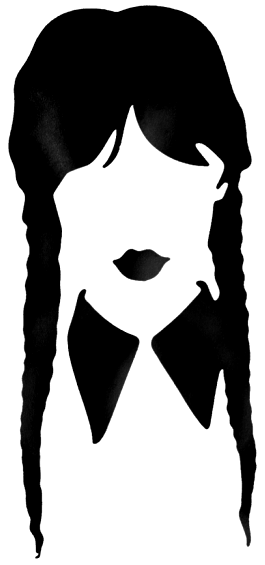
\includegraphics[height=1.35em]{figures/icons/mira-silhouette.png}}{}}}\enspace{\scshape\bfseries\color{black}Scene}\enspace\textperiodcentered\enspace{\bfseries #1}\pdblockheadingend{\itshape #2}}%
    \end{tcolorbox}\par\addvspace{8pt plus 2pt}%
  }%
  \long\def\xrefbox#1{\par\pd@settle\addvspace{4pt}\noindent\pd@marginhead{See also}{\small #1}\par\addvspace{4pt}}%
  % A generic "Thesis" margin label does not identify which claim matters.
  % Keep the prose; use an authored keyidea head only when it adds meaning.
  \long\def\pdthesis#1{\par\pd@settle\addvspace{6pt plus 1pt}\noindent#1\par\addvspace{6pt plus 1pt}}%
  \long\def\pullquote#1{\pdthesis{#1}}%
}
\makeatother

% Shared visual language for the seven analytical papers.
% This file defines marks, not layouts: every figure must still choose a grammar
% from its reader question.  The duplicate under whitepaper/figures is kept in
% lockstep for standalone Chapter I/II builds.
\usetikzlibrary{matrix,patterns.meta,shapes.geometric}

% ===========================================================================
% THE TYPOGRAPHIC LAW
% ===========================================================================
% Companion to the line-weight law in figures/pd-palette.tex (1px texture,
% 1.5px linework, 2px enclosure). Same shape of rule: name the roles, fix the
% values, one place.
%
% ONE SIZE. Every named text role in a figure is \pdfiglabelsize
% (= \footnotesize). Roles separate by WEIGHT, SLOPE, FAMILY and INK -- never
% by size. A fragment never writes a size command of its own; if a distinction
% needs making, it takes the role that makes it.
%
% Where the size comes from. Measured, not chosen:
%   \tiny  \scriptsize  \footnotesize  \small  \normalsize
%   5.23    6.97          8.72           9.55    10.46  pt   Book (10.5pt
%                                                            Pagella, 4.5in
%                                                            column, 7x10in)
%   5.98    7.97          8.97           9.96    10.91  pt   standalone chapter
%                                                            (11pt Latin Modern)
% \scriptsize renders at 6.97pt in the Book -- under figcheck's 7pt T1 floor
% before a single width promotion, so it is illegal by measurement, not taste.
% \footnotesize holds 8.72pt and still clears the floor at the 0.85 \resizebox
% limit craft-rules sets (7.41pt). It is also what the corpus already voted
% for: 78 of the 91 local font= declarations this law replaces were already
% \footnotesize, \footnotesize\bfseries or \footnotesize\itshape.
%
% \pdfigbasesize (= \small) is the tikzpicture's ambient size only, so an
% unstyled node is never SMALLER than a styled one; every named role steps
% down exactly one notch from it and none steps down twice.
%
% ONE FACE, AND IT IS THE DOCUMENT'S. \pdfiglabelfamily is empty by default,
% which means figure type inherits whatever face the document is setting --
% Palatino in the Book, Computer Modern in a standalone chapter. Figures
% agreeing with EACH OTHER is not the goal; figures agreeing with the
% paragraph beside them is. A fragment therefore never names a family. Not
% \sffamily (which resolves to Latin Modern Sans against a Computer Modern
% page and reads as a foreign object on it), not \rmfamily, not
% \fontfamily{...}. P18 in tikz_precheck.py is an error for exactly that.
% An edition MAY substitute a face -- the Swiss and technical editions set
% \pdfiglabelfamily to \pdgrotesk, because grotesk display is their declared
% character -- and it does so in ONE command in ONE file, so the substitution
% is a decision on the record rather than an accident in a fragment. The
% only family a fragment may ask for is the identifier one, and it asks for
% it by role (pd mono label / \pdfiglabelmono), never by \ttfamily.
%
% What the roles are, and what each one is for:
%   pd panel title        bold        the name of a panel
%   pd row label          bold        an actor/row name east of its lane
%   pd reverse row label  bold, cream a row name sitting on a dark band
%   pd axis label         regular     an axis title or a tick numeral
%   pd direct label       regular     a value or name riding its own mark
%   pd reverse label      regular, cream  a direct label on a dark band
%   pd mono label         mono        an identifier, path, or literal
%   pd verdict            bold        a terminal outcome stamp (CLEAR, REJECT)
%   pd note               italic      one aside per figure
%   pd legend             regular     a pgfplots legend entry
%   pd state / terminal / actor / artifact / decision   node text
%   pd axis               the whole pgfplots typographic block, one key
%   \pdfigsub             a gloss line under a heading INSIDE a node
%   \pdfigmath            math carrying a sub/superscript, inside a label
%
% A fragment that needs a compound style of its own composes it from a role
% above (`gate/.style={pd decision,minimum width=2cm}`), or, where no role
% fits, from the \pdfiglabel* handles here. It never writes a raw size
% command: P16 in skills/harbor-chartwork/scripts/tikz_precheck.py is an
% error for exactly that, and P10/P11 have been errors for \tiny and
% \scriptsize since before this law.
%
% What does NOT transfer from the screen rules these roles otherwise follow.
% The dataviz method those rules come from assumes an interactive chart: a
% tooltip carries any value a label could not fit, a filter row rescopes the
% view, hover lifts the hovered mark. A printed page has none of that, and the
% absence is not a defect to design around. The INTENT of the tooltip rule --
% "every value is reachable without gating" -- does transfer, and on this page
% it is discharged somewhere else: the value is in the caption, in the margin
% apparatus, or in the chapter's own worked example. So a label that will not
% fit inside its mark moves outside the mark or is dropped to the caption; it
% is never shrunk to fit, because there is no size below \footnotesize to shrink
% to, and never clipped. Do not add a hover affordance, a legend toggle, or a
% filter to a figure in this book.
%
% IDENTIFIERS GET ONE SPELLING. A key, a cell id, a file name or any other
% literal a reader could type is set in `pd mono label` (or \pdfiglabelmono
% inside a compound style), spelled exactly as the code spells it: sk_A, not
% skA and not sk with a subscript A; card0, not card-nought and not a Unicode
% subscript zero. A figure that shows the same identifier two ways has told
% the reader they are two things. The subscripted form belongs to MATHEMATICS
% ($\kappa_7$, an index into a sequence) and the literal form to CODE -- one
% figure may use both, for different objects, but never both for the same
% one. (A precheck for two spellings of one identifier inside a fragment is
% being added on another branch; this is the convention it will enforce.)
%
% SHAPE IS A CHANNEL, AND IT HAS TO SURVIVE THE PRINT SIZE. pd datum, pd
% focus datum and pd caution datum carry three different forms, because the
% house palette is three low-chroma print inks and every distinction it makes
% has to be doubled by something that is not colour. That only counts if the
% form is still legible at 2.1-2.7 pt: an edition that flattens all three to
% one form has removed the second channel and left the figure separating its
% classes by hue alone, which fails in greyscale and for a colour-blind
% reader. Any edition override that restyles a datum must keep three
% distinguishable forms, and must be checked on a render at 1.0x, not
% reasoned about from the point sizes.
%
% One screen rule that does NOT bind here, and why. "Text never wears the data
% colour" exists because a light categorical hue is illegible as text on a
% light surface. The house figure hues are print inks, not screen hues --
% hhink #1B1712, hhteal #00564C, hhamber #6B4500 -- and all three clear text
% contrast on cream, so a label MAY wear its series' ink to bind itself to a
% curve, which is direct labelling and saves a legend. The rule that survives
% is the reason behind it: text wears one of those three inks at full
% strength, or hhink!80!hhgray for recessive furniture, and nothing else. A
% tint of an ink (text=hhgray, text=hhteal!60) is not a role; it is a fade.
% ===========================================================================

\providecommand{\pdfiglabelfamily}{}            % an edition may set \pdgrotesk
\providecommand{\pdfiglabelsize}{\footnotesize} % every named text role
\providecommand{\pdfigbasesize}{\small}         % the picture's ambient size
\providecommand{\pdfiglabel}{\pdfiglabelfamily\pdfiglabelsize}
\providecommand{\pdfiglabelbold}{\pdfiglabel\bfseries}
\providecommand{\pdfiglabelitalic}{\pdfiglabel\itshape}
\providecommand{\pdfiglabelmono}{\pdfiglabelsize\ttfamily}
% The one role that is not a node style, because it lives INSIDE a node's text:
% the second line under a heading that glosses it ("reviewer role / obligation +
% capability + authority"). Every fragment that needed it reached for \tiny or
% \scriptsize, which is how seven \tiny and twelve \scriptsize survived P10/P11
% as hard errors in the corpus. It steps down by SLOPE and WEIGHT, not size, so
% it stays legible and stays legal, and it touches neither family nor ink --
% which is what lets it sit on a reversed node without vanishing.
\providecommand{\pdfigsub}{\mdseries\itshape}
% The one place the law's own size is not the right size, with the measurement
% that says so. A subscript is set at roughly 70% of its base, so math with a
% subscript inside a \pdfiglabelsize label renders its subscript at 5.98pt in a
% standalone chapter and 6.36pt in the Book -- under figcheck's 7pt T1 floor,
% measured, not estimated. One notch up puts the same subscript at 7.97pt and
% 7.64pt, over the floor, while the base glyph stays close enough to its
% neighbours that the label still reads as one label. Use it ONLY for a math
% group that carries a sub- or superscript; plain math takes the label's own
% size like any other text.
\providecommand{\pdfigmath}{\normalsize}

% ---------------------------------------------------------------------------
% THE GUIDE DASH, IN ABSOLUTE POINTS, IN ONE PLACE.
%
% `pd guide` used to read `line width=.45pt,densely dotted`. `densely dotted`
% expands to `dash pattern=on \pgflinewidth off 1pt`, and \pgflinewidth is read
% when the KEY is processed, not when the path is stroked. So the Swiss
% edition's `pd guide/.append style={draw=hhink!40,line width=.5pt}` widened the
% stroke and left the dash at the .45pt already baked into it. The canonical
% Book therefore shipped a 0.448pt dot on a 0.498pt stroke.
%
% Measured on the Book (Swiss, the built edition) at 1.0x / 150 dpi:
%   on 0.448pt = 0.93 device px -- UNDER ONE PIXEL
%   off 0.996pt = 2.08 px, period 3.01 px
%   peak ink per dot swings 0.173-0.345 (a 2.0x range) purely with where the
%     dot lands on the pixel grid; the line's weight is a rasteriser accident
%   the darkest pixel of the guide (0.30) is DARKER than every pixel of the
%     solid `pd hairline` (0.25/0.19) beside it, while its mean ink (2.3%) is a
%     quarter of the hairline's (8.9%) -- the two lines are not separated on any
%     axis a reader can name
%   declared separation from `pd hairline`: hhink!40 against hhink!45, 4.6% of
%     the grey scale
%
% So a fragment that used `pd guide` to mean "this line is not that line" was
% relying on ink that does not arrive on the page. Twenty-five of the corpus's
% thirty-six guide draws carry exactly that meaning.
%
% The replacement is stated absolutely and measures phase-STABLE: every dot
% renders at the same weight wherever it falls on the grid (peak column ink
% 0.808, invariant across twelve sub-pixel offsets). It is a macro rather than
% three numbers because an edition that restates one of them and not the others
% is how this defect happened. The geometry is a LEGIBILITY FLOOR, not an
% edition's character: an edition may move the guide's ink, and states the
% geometry through these two macros so it cannot half-restate it.
%
% Any dash in this corpus is stated in absolute points. The `dotted` family
% (`dotted`, `densely dotted`, `loosely dotted`) derives its on-length from the
% line width and is therefore banned -- P23 in tikz_precheck.py. `dashed` and
% its relatives are absolute (on 3pt off 3pt) and are fine.
\providecommand{\pdguidewidth}{.7pt}
% Three lengths, not one macro holding the whole key: pgfkeys splits a key list
% on `,` and `=` before expanding anything (so a macro carrying `dash
% pattern=...` is read as one key NAME), and TikZ's dash-pattern scanner reads
% the literal words `on`/`off` without expanding a macro that hides them. A
% dimension after each word does expand, which is the seam that works.
\providecommand{\pdguideon}{1.2pt}
\providecommand{\pdguideoff}{2.0pt}

\tikzset{
  pd figure/.style={font=\pdfiglabelfamily\pdfigbasesize,text=hhink},
  pd hairline/.style={draw=hhgray!78,line width=.5pt},
  pd rule/.style={draw=hhink,line width=.62pt},
  pd focus rule/.style={draw=hhteal,line width=1.05pt},
  pd caution rule/.style={draw=hhamber,line width=1.05pt},
  % Darker per dot than the hairline, lighter in mean ink than it: a guide is a
  % construction line the reader traces from a mark to an axis, so each dot has
  % to be a definite mark, while the line as a whole has to recede behind the
  % data. The hairline is the opposite -- continuous and faint. Those are the
  % two axes that now separate them, instead of 4.6% of the grey scale.
  pd guide/.style={draw=hhink!70,line width=\pdguidewidth,dash pattern=on \pdguideon off \pdguideoff},
  % A LATTICE is the rule work a figure stands on: column separators, row
  % baselines, a time grid. It is NOT dotted, and that is the point. Dotted
  % versus solid is a semantic channel -- it distinguishes a construction line
  % from a drawn edge -- and thirteen fragments were spending it on background
  % grid where it distinguishes nothing. A dash that carries no meaning is the
  % first ink a rasteriser is entitled to lose, and it did. A lattice is
  % continuous and quiet; a guide is discontinuous and definite. Use `pd guide`
  % only where the reader must see that the line is not a drawn edge.
  pd lattice/.style={draw=hhgray!52,line width=.4pt},
  pd arrow/.style={-{Stealth[length=2.0mm,width=1.25mm]},draw=hhink,line width=.68pt},
  pd focus arrow/.style={-{Stealth[length=2.0mm,width=1.25mm]},draw=hhteal,line width=.88pt},
  pd caution arrow/.style={-{Stealth[length=2.0mm,width=1.25mm]},draw=hhamber,line width=.88pt,dashed},
  pd row label/.style={font=\pdfiglabelbold,text=hhink,anchor=east},
  pd panel title/.style={font=\pdfiglabelbold,text=hhink,align=left},
  pd axis label/.style={font=\pdfiglabel,text=hhink!80!hhgray},
  % inner ysep is deliberately larger than inner xsep: at 1.5pt the descenders
  % of a last line (q, y, p, g) reach the bottom of the cream backing under
  % Computer Modern, where they clear it under Palatino. A label should not
  % need its own patch to hold its own tails, and the sensitivity is the
  % face's, not the fragment's.
  pd direct label/.style={font=\pdfiglabel,text=hhink,align=left,
    inner xsep=1.5pt,inner ysep=2.5pt,fill=hhpaper},
  pd note/.style={font=\pdfiglabelitalic,text=hhink!80!hhgray,align=left},
  pd tick/.style={draw=hhgray,line width=.45pt},
  pd datum/.style={circle,fill=hhink,draw=none,inner sep=2.1pt},
  pd focus datum/.style={circle,fill=hhteal,draw=hhpaper,line width=.55pt,inner sep=2.5pt},
  pd caution datum/.style={diamond,fill=hhamber,draw=hhpaper,line width=.55pt,inner sep=2.5pt},
  pd state/.style={draw=hhink,line width=.62pt,fill=hhsand!30,rounded corners=1.5pt,
    font=\pdfiglabel,inner xsep=8pt,inner ysep=6pt,align=center,minimum height=9mm},
  pd terminal/.style={pd state,double,double distance=1.2pt},
  pd actor/.style={draw=hhink,line width=.62pt,fill=hhpaper,rounded corners=1.5pt,
    font=\pdfiglabel,inner xsep=8pt,inner ysep=5pt,align=center},
  pd artifact/.style={draw=hhgray!80,line width=.55pt,fill=hhsand!30,
    font=\pdfiglabel,inner xsep=8pt,inner ysep=5pt,align=center},
  pd boundary/.style={draw=hhgray!70,line width=.55pt,dashed,rounded corners=2pt},
  % These three are pale washes: they are frequently layered on top of `pd
  % state` (directly, or via a compound style like `cell`), whose swiss-edition
  % override (figures/pd-figure-language-swiss.tex) appends text=hhpaper for the
  % common case of a solid, saturated fill. A pale wash is the opposite case --
  % text must stay dark ink regardless of what came before it in the style
  % list, so each one restates text=hhink explicitly rather than relying on
  % whatever was inherited.
  pd focus fill/.style={fill=hhteal!24,draw=hhteal!65,line width=.4pt,text=hhink},
  pd caution fill/.style={fill=hhamber!26,draw=hhamber!70,line width=.4pt,text=hhink},
  pd neutral fill/.style={fill=hhsand!40,draw=hhgray!65,line width=.4pt,text=hhink},
  pd ink fill/.style={fill=hhink,draw=hhink,line width=.4pt,text=hhpaper},
  pd hatch/.style={pattern={Lines[angle=45,distance=4pt,line width=.28pt]},pattern color=hhgray!55},
  % --- roles the corpus was inventing locally, now named -------------------
  % Each is built ON TOP of the role it varies, so an edition's .append style
  % on the parent reaches it without the edition file having to list it.
  pd decision/.style={pd state,diamond,aspect=1.55,font=\pdfiglabelbold,
    minimum height=0pt,inner xsep=3pt,inner ysep=3pt},
  % A shade more side bearing than its parent: a monospace glyph box overhangs
  % its own advance width, so the cream backing at the parent's 1.5pt clipped
  % the last character of a long identifier.
  pd mono label/.style={pd direct label,font=\pdfiglabelmono,inner xsep=2.5pt,inner ysep=2.5pt},
  pd verdict/.style={pd direct label,font=\pdfiglabelbold},
  pd reverse label/.style={pd direct label,text=hhpaper,fill=none},
  pd reverse row label/.style={pd row label,text=hhpaper},
  pd legend/.style={font=\pdfiglabel,text=hhink,draw=none,fill=none},
  % A KIND TAG names what a row or column IS, rather than what it says: an
  % audience ("for the operator"), a category, a running head. craft-rules S6
  % already reserves small caps for exactly this, and small caps is the
  % smallest effective difference that marks a change in kind -- it needs no
  % size drop, no second colour and no box.
  pd kind tag/.style={pd axis label,font=\pdfiglabel\scshape,align=right},
  % A BADGE is a short boxed fact riding beside a row -- a part and chapter
  % range, a version, a count. Hairline edge, no fill: it is a label with a
  % boundary, not a region.
  pd badge/.style={pd hairline,font=\pdfiglabel,text=hhink,align=center,
    inner sep=2.4pt,fill=none},
}

% The pgfplots half of the same law. Before this existed, every plot fragment
% restated title style/label style/tick label style by hand, and they disagreed
% -- four said the tick numerals were hhink!80!hhgray, three said hhgray, and
% the axis rule was drawn four different ways. `pd axis` is the one place now.
% The axis line is `pd hairline` because an axis is reference furniture, not
% data: heavy for data, light for the frame that carries it.
\ifdefined\pgfplotsset
\pgfplotsset{
  pd axis/.style={
    title style={font=\pdfiglabelbold,text=hhink,yshift=-2pt},
    label style={font=\pdfiglabel,text=hhink!80!hhgray},
    tick label style={font=\pdfiglabel,text=hhink!80!hhgray},
    legend style={pd legend},
    axis line style={pd hairline},
    tick style={pd tick},
  },
}
\fi

% Small reusable marks.  They deliberately avoid prose-bearing boxes.
\newcommand{\pdfigaxis}[4]{%
  \draw[pd rule,-{Stealth[length=1.65mm,width=1.05mm]}] (#1,#2) -- (#3,#2);
  \node[pd axis label,anchor=west] at (#3,#2) {#4};
}
\newcommand{\pdfigvaxis}[4]{%
  \draw[pd rule,-{Stealth[length=1.65mm,width=1.05mm]}] (#1,#2) -- (#1,#3);
  \node[pd axis label,anchor=south,align=center] at (#1,#3) {#4};
}

% ---------------------------------------------------------------------------
% Editions. The Book sets \pdedition (maritime | swiss | technical) and the
% matching override file restyles the same names, so one drawing renders in
% each edition's character. Standalone chapters have no edition. An edition
% changes the FAMILY (via \pdfiglabelfamily) and the character of the marks;
% it never changes the size, because the size is the law above.
% ---------------------------------------------------------------------------
\ifdefined\pdedition\IfFileExists{figures/pd-figure-language-\pdedition.tex}{\input{figures/pd-figure-language-\pdedition}}{}\fi


% The proof-obligation markers (\Closed/\Partial/\Open) come from
% figures/pd-pedagogy.tex (\input above), so this chapter has them available
% for the implementation-status appendix it does not yet carry -- without a
% second definition of its own. This skeleton pass uses none of them.


% ─── Listings Setup ─────────────────────────────────────────────────────
\lstdefinestyle{proverif}{
  language=C,
  backgroundcolor=\color{codebg},
  frame=single,
  rulecolor=\color{codeframe},
  basicstyle=\ttfamily\small,
  keywordstyle=\color{darkblue}\bfseries,
  commentstyle=\color{darkgreen}\itshape,
  stringstyle=\color{accent},
  numbers=left,
  numberstyle=\tiny\color{gray},
  numbersep=8pt,
  breaklines=true,
  showstringspaces=false,
  tabsize=2,
  xleftmargin=15pt,
  xrightmargin=5pt,
  framexleftmargin=15pt,
  captionpos=b
}
\lstset{style=proverif}

% ─── Theorem Environments ──────────────────────────────────────────────
\theoremstyle{definition}
\newtheorem{definition}{Definition}[section]
\newtheorem{theorem}{Theorem}[section]
\newtheorem{lemma}{Lemma}[section]
\newtheorem{property}{Property}[section]

% ─── Header/Footer ───────────────────────────────────────────────────────
\pagestyle{fancy}
\fancyhf{}
\fancyhead[L]{\small\textit{The Sealed Harbor}}
\fancyhead[R]{\small\thepage}
\fancyfoot[C]{\footnotesize\color{hhgray} Port Daddy Coordination Papers \textperiodcentered\ Chapter~\pdchapternumber\ of \pdchaptercount}
\renewcommand{\headrulewidth}{0.4pt}
\renewcommand{\footrulewidth}{0pt}

% ─── Title ──────────────────────────────────────────────────────────────────
\title{
  \vspace{-1cm}
  {\Large\textsc{Port Daddy Coordination Papers --- Chapter~\pdchapternumber\ of \pdchaptercount}}\\[
0.5cm]
  \rule{\textwidth}{0.5pt}\\[0.3cm]
  {\LARGE\textbf{The Sealed Harbor:}}\\[0.2cm]
  {\Large Mutually Confidential Computation with\\Explicit, Gated, Bounded Releases}\\[0.3cm]
  \rule{\textwidth}{0.5pt}
}
\author{
  \textbf{Erich Owens}\\[0.2cm]
  Curiositech LLC\\[0.2cm]
  \texttt{engineering@portdaddy.dev}
}
\date{September 2026\\Version 1.0 (textbook edition)}
% ─── Document ────────────────────────────────────────────────────────────
% Hyperlink and cross-reference discipline (must stay last in the preamble).
% Shared hyperlink and cross-reference discipline for the Book and its chapters.
% Load this LAST in every preamble: cleveref must follow hyperref and amsthm.
% hyperref itself is loaded earlier with [backref=page] (a load-time option).
% Twin copy under whitepaper/figures/ (byte-identical; checked by
% scripts/generate-mega-whitepaper.test.mjs).
%
% What a reader gets: live links on chapter titles, section numbers, theorems,
% figures, tables, equations, page numbers, and citations; PDF bookmarks three
% levels deep; and, at the end of every bibliography entry, the pages that cite it.
% Links are quiet: a warm dark ink one step lighter than body text, so the
% four part hues keep their meaning and an inline chapter title never competes
% with the part it sits in. Chrome pages (the front-matter map, part openers)
% recolor their own links locally.
\hypersetup{
  colorlinks=true,
  linkcolor=pdinkmuted,
  citecolor=pdinkmuted,
  urlcolor=pdinkmuted,
  filecolor=pdinkmuted,
  anchorcolor=pdink,
  bookmarksnumbered=true,
  bookmarksdepth=3,
  bookmarksopen=true,
  bookmarksopenlevel=1,
  breaklinks=true,
  linktoc=all,
  pdfauthor={Erich Owens},
  pdftitle={\pdchaptertitle},
  pdfsubject={\pdeditiontitle: \pdeditionsubtitle},
}

% Title-based chapter references. \pdchaplink{prefix}{text} is a live link to
% the chapter inside the Book (the Book's preamble defines it before loading this
% file); in a standalone chapter it is plain text. Prose uses \pdchapref, which
% sets the title in italics; the locator map uses \pdchaplink directly.
\providecommand{\pdchaplink}[2]{#2}
\DeclareRobustCommand{\pdchapref}[2]{\pdchaplink{#1}{\emph{#2}}}

% \ifpdbook -- true in the assembled Book, false in a standalone paper.
%
% WHY THIS EXISTS. A drawing that two chapters both \input prints twice in the
% Book, under two figure numbers. The fix is for the chapter that develops the
% idea to keep the figure and the other to point at it -- but a standalone
% paper has nowhere to point, and rewriting the prose outright removed five
% figures from harbor-economy-whitepaper.pdf and left it telling a conference
% reader that a ceremony is "drawn in The Federated Harbor", a document that
% reader does not have.
%
% So the divergence is per-build. A CONDITIONAL and not a two-argument macro:
% the generator inlines each \input, so a figure branch is a whole table or
% tikzpicture, and as a macro argument that is scanned as one token list --
% which is how \pdinbook produced "runaway argument" on the first attempt.
% \ifpdbook skips the untaken branch at the TeX level instead.
%
% Declared unconditionally and defaulting FALSE, which is the standalone
% answer. The Book's preamble sets \pdbooktrue immediately after loading
% this file. A guard here would have to mention \ifpdbook or \newif inside a
% branch TeX may skip, and a conditional token in skipped text is counted as
% a nested \if -- which is how two attempts at a guard both produced
% "Incomplete \ifdefined". Ordering is cheaper than cleverness.
\newif\ifpdbook

% cleveref: "Theorem 3.1", "Figure 2.4", "Section 1.3", capitalised, never
% abbreviated, with the whole phrase clickable. Names are declared explicitly
% because the theorem environments are created before this file is loaded.
\usepackage[nameinlink,capitalise,noabbrev]{cleveref}
\crefname{pdchapter}{Chapter}{Chapters}
\crefname{part}{Part}{Parts}
\crefname{appendix}{Appendix}{Appendices}
\crefname{definition}{Definition}{Definitions}
\crefname{theorem}{Theorem}{Theorems}
\crefname{lemma}{Lemma}{Lemmas}
\crefname{proposition}{Proposition}{Propositions}
\crefname{corollary}{Corollary}{Corollaries}
\crefname{conjecture}{Conjecture}{Conjectures}
\crefname{property}{Property}{Properties}
\crefname{protocol}{Protocol}{Protocols}
\crefname{lsprotocol}{Protocol}{Protocols}
\crefname{stpprotocol}{Protocol}{Protocols}
\crefname{heprotocol}{Protocol}{Protocols}
\crefname{remark}{Remark}{Remarks}
\crefname{lstlisting}{Listing}{Listings}
\crefname{exercise}{Exercise}{Exercises}
\crefname{solution}{Solution}{Solutions}
\Crefname{pdchapter}{Chapter}{Chapters}
\Crefname{lstlisting}{Listing}{Listings}
\Crefname{exercise}{Exercise}{Exercises}
\Crefname{solution}{Solution}{Solutions}

% Back-references: "^ Cited on pages 12, 40, and 87." after every bibliography
% entry, each page number a live link back to the page that cited the work.
% Distinct pages only (#3/#4).
%
% The page numbers used to be wrapped in \color{hhgray} along with the words,
% which painted over the link colour hyperref had just given them: the links
% were there -- 29 annotations on a typical bibliography page -- and looked
% exactly like the grey prose around them, so nobody knew they could click.
% Restoring the quiet link colour would not have fixed it either; pdinkmuted
% against hhgray is 1.53:1, which is no signal at footnote size.
%
% So the numbers take pdcobalt (7.55:1 on the cream, and a hue a reader cannot
% mistake for grey), and the line opens with the return arrow this book already
% uses to send a solution back to its exercise. This is a deliberate exception
% to the quiet-link discipline above, and the reason is that back-matter
% navigation is the one place where the link IS the content: in prose the
% surrounding sentence tells you a phrase is a destination, and in a
% bibliography nothing does.
\renewcommand*{\backref}[1]{}
\renewcommand*{\backrefalt}[4]{%
  \ifcase #3\relax
  \or {\footnotesize{\color{hhgray}$\uparrow$~Cited on page}~{\hypersetup{linkcolor=pdcobalt}#4}{\color{hhgray}.}}%
  \else {\footnotesize{\color{hhgray}$\uparrow$~Cited on pages}~{\hypersetup{linkcolor=pdcobalt}#4}{\color{hhgray}.}}%
  \fi}
\renewcommand*{\backrefsep}{, }
\renewcommand*{\backreftwosep}{ and }
\renewcommand*{\backreflastsep}{, and }

\begin{document}
\pdopensolutions
\setlength{\emergencystretch}{2em}
\maketitle
\thispagestyle{empty}
\vspace{1cm}
% ---------------------------------------------------------------------------
% The Sealed Harbor: chapter body, part 1 (problem, design, noninterference,
% enforceability). Folds research paper 4 (R9, R10, R11) and the clean-room
% appendix into the chapter's own voice. Part 2 carries conservation,
% detection, the leakage budget, limitations, recitation, and exercises.
% ---------------------------------------------------------------------------
\section{Two owners, one answer}\label{sec:sealed-problem}
\noindent\emph{Express lane: a sealed room lets an agent compute on data its
owner will not hand over, and the room's promise is not ``nothing leaks'' but
``every release is explicit, gated, and bounded''; the four claims that make
that promise provable are Theorems~\ref{thm:sealed-noninterference},
\ref{thm:sealed-conservation}, and \ref{thm:sealed-power}, plus the
controllability theorem of \pdchapref{swk}{The Single-Writer Kernel}, and the
leakage they leave is the account of Section~\ref{sec:sealed-budget}.}
\paragraph{The scene.}
Derek owns sensitive financial data $D$. Erin owns a valuable agent system $M$:
weights, prompts, skills, tools, orchestration. Both want the answer
$y=f_M(D)$. Neither will hand over the crown jewels: Derek must not receive $M$,
Erin must not receive $D$, and the cloud operator hosting the computation must
receive neither -- three parties, three sight-lines, one boundary that must
seal all of them at once, drawn in Figure~\ref{fig:sealed-three-principals}.
% Fragment: fig-sealed-three-principals.tex -- the three parties who must
% never see each other's plaintext, and the one boundary that seals all
% three lines of sight at once.
%
% Reader question: which three parties must never see each other's
% plaintext, and what single mechanism seals all three lines of sight?
% Claim: Derek, Erin, and the cloud operator form a triangle of mutual
% "must not see" constraints, and one boundary (not three separate ones)
% seals every edge of that triangle at once.
% Evidence: "The scene" paragraph, website-v2/public/whitepaper/
% sealed-harbor.tex, Sec. sealed-problem ("Derek owns sensitive financial
% data D. Erin owns a valuable agent system M... Derek must not receive
% M, Erin must not receive D, and the cloud operator hosting the
% computation must receive neither.").
% Must distinguish: three named parties, not two -- the counter-read this
% figure exists to correct is a reader who thinks only Derek-versus-Erin
% needs separating and forgets the host; and one enclosing boundary, not
% three pairwise fences, since the room seals all three sight-lines with a
% single mechanism.
% Grammar chosen: relation map, three principal nodes in a triangle with
% explicit "must not see" edges on every side, the whole triangle enclosed
% by one trust-boundary rectangle (the S12 Dolev-Yao convention already
% used for the room elsewhere in this chapter).
% Grammar rejected: three separate two-party boxes (Derek|Erin,
% Derek|cloud, Erin|cloud) -- that draws three fences where the chapter's
% claim is exactly that one mechanism does the sealing, not three.
% Five-second test: count the boundaries drawn -- one rectangle, around
% all three parties and all three edges, not a fence per pair.
% QA: beauty_lint warns B7 (sub-point near-alignment noise between
% rotated edge-tags and node centres); justified, not fixed.
\begin{figure}[H]
\centering
\pdfigurehue{pdcobalt}%
\begin{tikzpicture}[pd figure,x=1cm,y=1cm]
  \node[pd focus outline,minimum width=2.6cm,align=center]
    (DEREK) at (0,3.6) {Derek\\\itshape holds $D$};
  \node[pd focus outline,minimum width=2.6cm,align=center]
    (ERIN) at (6.2,3.6) {Erin\\\itshape holds $M$};
  \node[pd focus outline,minimum width=2.9cm,align=center]
    (CLOUD) at (3.1,0.4) {cloud operator\\\itshape holds neither};
  \draw[pd breach rule] (DEREK) -- (ERIN);
  \node[pd tag,anchor=south] at ($(DEREK)!0.5!(ERIN)$) {must not see};
  \draw[pd breach rule] (DEREK) -- (CLOUD);
  \node[pd tag,anchor=east,rotate=52] at ($(DEREK)!0.5!(CLOUD)$) {must not see};
  \draw[pd breach rule] (ERIN) -- (CLOUD);
  \node[pd tag,anchor=west,rotate=-52] at ($(ERIN)!0.5!(CLOUD)$) {must not see};
  \begin{scope}[on background layer]
    \node[pd trust boundary,fit={(DEREK)(ERIN)(CLOUD)},inner sep=16pt]
      (ROOM) {};
  \end{scope}
  \node[pd title,anchor=south west] at (ROOM.north west) {the sealed room};
  \node[pd note,anchor=north,align=center,text width=6.6cm]
    at (3.1,-1.55) {one boundary seals all three sight-lines at once};
\end{tikzpicture}
\caption{The room must keep Erin's model from Derek, Derek's data from Erin, and both from the cloud operator. One mechanism must satisfy all three separations. [internal]}
\label{fig:sealed-three-principals}
\end{figure}

The technical question is what the execution environment can guarantee when
the data owner and agent owner distrust each other. A computational contract
specifies permitted releases; it does not settle their legal relationship.
The systems literature answered a narrower version first: Ryoan
\pdcite{ryoan16} confines a proprietary module inside an attested enclave so that
a data owner and a code owner who distrust each other both keep their secrets.
Ryoan buys its confinement with a module that sees its input once and keeps no
state between requests in its confinement model. This chapter instead studies
persistent tool-calling workloads and explicit releases. Table~\ref{tab:sealed-ryoan}
compares the chosen mechanisms; it is not an impossibility claim about other
sandbox architectures.
The other end of that design space is worth naming in the same breath, because it
is where most deployments actually sit: SCONE \pdcite{scone16} puts an ordinary
Linux container inside SGX and asks almost nothing of the application, which makes
it adoptable in a way Ryoan is not, and buys correspondingly less --- it protects
the workload from the host, not the data owner from the code owner, and a
container free to open sockets can carry $D$ out through any of them. Between the
two lies the gap this chapter works in: the stateful, non-DAG, tool-calling
workload whose releases need an explicit policy beyond transparent execution.
A mediated gate and accounting ledger are this design's proposal, not the only
possible solution. A single writer orders accounting; it cannot, by itself,
provide confinement or determine what an output reveals.
\begin{table}[H]\centering\footnotesize
\caption{Different workload and observation models. Ryoan uses request-oriented
confinement; the proposed sealed room adds explicit releases and cross-job
accounting for a persistent agent. Neither closes every side channel.}
\label{tab:sealed-ryoan}
\begin{tabularx}{\textwidth}{@{}>{\raggedright\arraybackslash}p{2.2cm} >{\raggedright\arraybackslash}X >{\raggedright\arraybackslash}X@{}}
\toprule
 & Ryoan & The sealed room \\
\midrule
Workload shape & a request-oriented module, input seen once, no persistent state & a looping, tool-calling agent with state across steps \\
How leakage is bounded & confinement in the enclave plus fixed-size outputs & explicit gated releases, priced by an $\varepsilon$-ledger and a $q\cdot b$ bit budget \\
Taint granularity & the whole module & the slot: every release is a declassification event \\
Model access & the module's code is sealed; no query interface & the model runs inside the domain and is observed only through the contracted query and output interface \\
Multi-job accounting & none; each request stands alone & the ledger sums spend across jobs and refuses the overdraw \\
Evasion & constrained within its stated confinement model & canaries detect specified alternatives with stated power, not every evasion \\
Timing & out of scope & declared out of model; padded and scheduled, not closed \\
\bottomrule
\end{tabularx}
\end{table}
\paragraph{Why blocking tainted outputs is insufficient.}
Consider a proposed ``silicon-enforced NDA'': tag Erin's agent the moment it
reads Derek's data, drop any tainted egress packet, and declare that the data
``mathematically cannot phone home.'' The first job of this chapter is to say
why that sentence is false, and the second is to prove the sentence that
replaces it.
\begin{pdexample}{What ``Nothing Leaks'' Costs, in Bits}
\setlength{\parskip}{4pt plus 1pt}
Price the three candidate designs on the chapter's own toy release --- the one
Theorem~\ref{thm:sealed-noninterference} will later check exhaustively --- and
you can do the whole comparison in your head. Derek's secret is one of
$\{0,1,2,3\}$, so it carries $\log_2 4 = 2$ bits, and the contracted release is
\[
g(s)=s\bmod 2,
\]
which takes two values and therefore carries exactly $1$ bit
--- and, since $s$ written in binary has its parity in the low position, that
release is literally one of the secret's two bits.

Now count. An honest gate
hands Erin $1$ of those $2$ bits: the bit Derek sold her, and no more.

The leaky gate of the mutation suite, which forwards $s$ itself, hands over $2$ ---
the whole secret, which is why the checker catches it four steps in.

And the taint tracker of the pitch above, run \emph{soundly} at token granularity, has
to mark the parity bit as tainted by the secret it was computed from and drop
it, so Erin gets $0$ bits and the engagement has nothing left to deliver to
her.

The $0$-bit design blocks the contracted answer along with the secret; the
other horn, the tracker that lets the parity through, cannot then certify that
what the worker submitted was $s$ rather than some $f(s)$ it chose.

Every honest design in this chapter therefore lives in the middle column, and the
rest of the chapter is the arithmetic of how wide that column is allowed to
get.
\end{pdexample}

\begin{pdclaim}{Empirical hypothesis}{Token-Level Taint through a Language Model Is Not Soundly Definable}
\setlength{\parskip}{4pt plus 1pt}
\label{hyp:sealed-taint}
A taint tracker over a generative model faces a binary choice: mark every
output token as tainted by everything the model read, which is useless, or
miss semantic flows, which is unsound. The model taints everything it writes
with everything it read.

This is a design rationale, not a theorem, and it is
the one decisive statement in this chapter that carries no proof and no
script.

It rests on the well-known static-analysis result beneath it, that
certifying implicit flows soundly forces exactly this dichotomy: the label
creep of the Denning certification lattice \pdcite{denning77} and the extra
restrictiveness a sound purely dynamic monitor must accept relative to a static
one \pdcite{rs10}.

No sound token-granularity flow analysis for a generative model
is known; the burden of exhibiting one falls on any design that assumes it.
\end{pdclaim}

A secret can ride out in wording, punctuation, error messages, output length,
or timing; no regular expression, scanner, or second model can certify that
arbitrary prose contains no secret. And an ordinary remote model API is
\emph{itself} a trusted reader of plaintext: cryptography cannot repair
sending Derek's data to a third party's inference endpoint.

The architecture therefore controls the \emph{channel}, not the token. It
converts the question a security officer will actually ask, \emph{how do I know
the wall has no other holes?}, into four provable claims: the gate is the only
hole (Section~\ref{sec:sealed-noninterference}); the gate sits on the only
boundary that can be enforced at all
(Section~\ref{sec:sealed-enforceability}); what passes through it is metered by
a conserved budget (Section~\ref{sec:sealed-conservation}); and canary
detection has conditional power and model-based stopping estimates
(Section~\ref{sec:sealed-detection}). Section~\ref{sec:sealed-budget} composes
the four into a single leakage account, and
Section~\ref{sec:sealed-limitations} states, at equal prominence, what none of
this promises.

\section{One work order, two fences, two gates}\label{sec:sealed-design}

\paragraph{The work order.}
Both principals sign the same contract before any key is released:
{\small\[
\begin{aligned}
C=\bigl\langle\, & H(\text{data manifest}),\,H(\text{agent bundle}),\,H(\text{runtime}),\,H(\text{policy}),\\
& \text{function},\,\text{tools},\,\text{recipients},\,\text{output schemas},\,\text{budgets},\\
& \text{retention},\,\text{validators},\,\text{payment},\,\text{liability}\,\bigr\rangle.
\end{aligned}
\]}
Read the tuple in order. The four hashes pin the data manifest, the agent
bundle, the measured runtime, and the policy; function and tools fix what may
run and what it may call; recipients and output schemas fix who may receive a
result and in what shape; budgets bound output bits, queries, and time;
retention fixes key destruction; validators name the success evidence and the
dispute procedure; payment and liability are the guarantee. Any change makes a
new hash and requires both signatures. It is a work unit in the sense of \pdchapref{swk}{The Single-Writer
Kernel}: the case file that outlives every process that touches it.
Figure~\ref{fig:sealed-work-order-schema} groups the tuple's thirteen
fields by the five roles just named.

% Fragment: fig-sealed-work-order-schema.tex -- the work order C's
% thirteen fields, grouped by role, as an annotated record schema.
%
% Reader question: what exactly does the one contract both principals
% sign pin down, and what forces a re-sign?
% Claim: the work order's thirteen fields fall into five roles -- pins,
% permissions, recipients, bounds, and remedies -- and changing any one
% field changes the hash, which invalidates both signatures.
% Evidence: "The work order" paragraph, website-v2/public/whitepaper/
% sealed-harbor.tex, Sec. sealed-design (the tuple C, and "Read the tuple
% in order..."; "Any change makes a new hash and requires both
% signatures.").
% Must distinguish: the chapter's own five-way grouping (not a flat list
% of thirteen fields); and, within "pins," that a hash pins the runtime's
% attested MEASUREMENT, not its live state -- the counter-read this
% figure exists to preempt.
% Grammar chosen: block stack (tpl-block-stack), one band per role, the
% record's own field names on the right, a one-line gloss closing each
% band -- fields "sit inside" a role the way a block stack's layers sit
% on each other, and no arrows are needed since containment is the claim.
% Grammar rejected: a flat itemized list of thirteen fields -- loses the
% five-way grouping that is the chapter's own organizing idea and that
% Exercise-level readers are expected to reproduce from memory.
% Five-second test: name the one field that pins the runtime, and say
% what it pins (a measurement, not a live state).
% QA: beauty_lint warns B2 in maritime/technical (row-divider hairlines
% 1.0-1.4pt from the last wrapped line of a gloss) and B7 (sub-point
% alignment noise across the five bands' left-column baselines);
% justified, not fixed.
\begin{figure}[H]
\centering
\pdfigurehue{pdcobalt}%
\begin{tikzpicture}[pd figure,x=1cm,y=1cm]
  \def\w{11.2}  \def\h{2.15}
  \foreach \i/\name/\fields/\gloss/\s in {%
    4/{pins}/{$H(\text{data})$, $H(\text{agent})$, $H(\text{runtime})$, $H(\text{policy})$}/{four hashes -- each pins an attested measurement, not the live thing}/{pd focus fill},
    3/{permissions}/{function, tools}/{fixes what may run and what it may call}/{pd neutral fill},
    2/{recipients}/{recipients, output schemas}/{fixes who may receive a result, and in what shape}/{pd neutral fill},
    1/{bounds}/{budgets, retention}/{bounds output bits, queries, and time; retention fixes key destruction}/{pd neutral fill},
    0/{remedies}/{validators, payment, liability}/{validators name the success evidence and dispute procedure; payment and liability are the guarantee}/{pd neutral fill}}{
      \draw[\s] (0,{\i*\h}) rectangle (\w,{\i*\h+\h});
      \node[pd title,anchor=north west,text width=2.3cm] at (0.22,{\i*\h+\h-0.18}) {\name};
      \node[pd label,anchor=north west,text width=3.55cm,align=left]
        at (2.75,{\i*\h+\h-0.18}) {\fields};
      \node[pd label,text=pdinkmuted,anchor=north west,text width=4.55cm,align=left]
        at (6.55,{\i*\h+\h-0.18}) {\gloss};}
  \node[pd kind] at (1.35,{5*\h+0.35}) {role};
  \node[pd kind] at (4.5,{5*\h+0.35}) {fields};
  \node[pd kind] at (8.8,{5*\h+0.35}) {what it fixes};
  \node[pd note,anchor=north west,align=left,text width=10.9cm]
    at (0.22,-0.42) {any change to any field makes a new hash for $C$ and requires both Derek's and Erin's signatures again};
\end{tikzpicture}
\caption{The work order binds measurements, permitted execution, recipients, limits, and remedies. Hashes identify attested measurements, not live query-time state. Any field change requires both principals to sign again. [internal]}
\label{fig:sealed-work-order-schema}
\end{figure}


\paragraph{Dual-attested key release.}
The workload boots in a confidential virtual machine and creates an ephemeral
job key with fresh attestation evidence binding runtime, policy, worker image,
key, nonce, and epoch. Derek and Erin \emph{independently} verify the
attestation; Derek's key broker releases the data key only to the approved
measurement, and Erin's key broker releases the model and skill key under the
same condition, the attester, verifier, and relying-party pattern of IETF RATS
\pdcite{rats}. The job then runs with no ambient network or credentials. Neither
principal, and not the cloud operator, can read the other's plaintext: the room
is sealed from three sides at once.

Figure~\ref{fig:sealed-dual-attestation} draws the ceremony as a sequence:
one attestation evidence bundle, appraised twice and independently, each
broker releasing its own key off its own appraisal alone.

% Fragment: fig-sealed-dual-attestation.tex -- the dual-attested key release
% ceremony of Sec. sealed-design as a full sequence diagram.
%
% Reader question: in what order do the two owners verify attestation and
% release keys, and what state exists once both have released?
% Claim: one attestation is produced once, forwarded once, but appraised
% TWICE -- once against Derek's approved measurement, once against Erin's,
% independently -- and each key broker releases its own key only off its
% own appraisal; the job then runs with no ambient network or credentials.
% Evidence: "Dual-attested key release" paragraph, website-v2/public/
% whitepaper/sealed-harbor.tex, Sec. sealed-design ("fresh attestation
% evidence binding runtime, policy, worker image, key, nonce, and epoch...
% Derek and Erin independently verify the attestation... the attester,
% verifier, and relying-party pattern of IETF RATS") [internal, rats].
% Must distinguish: the RATS roles by name (attester = the init agent that
% produces and forwards evidence; verifier = the appraisal step; relying
% party = each key broker's release decision) from the hardware root of
% trust that actually signs the evidence, which RATS treats as part of the
% attesting environment but the ceremony gives its own lifeline; above all,
% that messages 4 and 5 are two INDEPENDENT appraisals of the SAME evidence,
% not one shared verification step fanned out to two recipients -- the
% counter-read this figure is drawn to preempt.
% Grammar chosen: message-sequence ladder, five lifelines, numbered
% forward-sloped messages keyed to a ruled legend naming what each one
% binds (tpl-message-ladder). Five lifelines use short, wrapped headers;
% the entire diagram stays in the 4.5 in body column at normal label size.
% Grammar rejected: a 3-lifeline ladder (CVM, Derek's broker, Erin's
% broker) matching the register row's original recommendation -- collapses
% the hardware root of trust into the CVM and the verifier into each
% broker, exactly the "one shared verification step" misreading this
% figure exists to correct.
% Five-second test: count the appraisal arrows leaving the verifier --
% there are two, one per broker, not one arrow that forks.
% QA: inspect the assembled page. Legacy fragment approvals do not cover
% current type metrics, margin ownership, or the clearance around messages.
\begin{figure}[H]
\centering
\pdfigurehue{pdcobalt}%
\begin{tikzpicture}[pd figure,x=1cm,y=1cm]
  \def\dy{1.05}   \def\gap{2.15}   \def\rows{7}
  \foreach \i/\name/\role in {%
    0/{hardware}/{root of trust},
    1/{init agent}/{attester (CVM)},
    2/{verifier}/{RATS appraisal}}{
    \node[pd state,minimum width=1.85cm] (h\i) at ({\i*\gap},0) {\name};
    \node[pd label,text=pdinkmuted,anchor=north,text width=1.8cm,align=center] at ({\i*\gap},-0.52) {\role};
    \draw[pd guide] ({\i*\gap},-1.30) -- ({\i*\gap},{-\rows*\dy-0.55});}
  \foreach \i/\name/\role in {%
    3/{Derek}/{relying party},
    4/{Erin}/{relying party}}{
    \node[pd state,minimum width=1.85cm] (h\i) at ({\i*\gap},0) {\name};
    \node[pd label,text=pdinkmuted,anchor=north,text width=1.8cm,align=center] at ({\i*\gap},-0.52) {\role};
    \ifnum\i=4
      \draw[pd guide] ({\i*\gap},-1.30) -- ({\i*\gap},-4.45);
      \draw[pd guide] ({\i*\gap},-5.95) -- ({\i*\gap},{-\rows*\dy-0.55});
    \else
      \draw[pd guide] ({\i*\gap},-1.30) -- ({\i*\gap},{-\rows*\dy-0.55});
    \fi}
  \foreach \a/\b/\k in {1/0/1, 0/1/2, 1/2/3, 2/3/4, 2/4/5, 3/1/6, 4/1/7}{
    \pgfmathsetmacro{\ytail}{-\k*\dy-0.43}
    \pgfmathsetmacro{\yhead}{-\k*\dy-0.67}
    \node[pd focus badge] (m\k) at ({(\a+\b)*\gap/2},{-\k*\dy-0.55}) {\k};
    \draw[pd focus arrow,pd to badge] ({\a*\gap},\ytail) -- (m\k);
    \draw[pd focus arrow,pd from badge] (m\k) -- ({\b*\gap},\yhead);}
  \begin{scope}[on background layer]
    \node[pd panel,fit={(m4)(m5)},inner xsep=10pt,inner ysep=7pt] (appraisals) {};
  \end{scope}
  \node[pd label,anchor=west,text width=2.2cm,align=left]
    at ([xshift=6pt]appraisals.east) {independent appraisals};
  \node[pd terminal,minimum width=3.6cm,align=center,text width=3.2cm]
    (SEALED) at ({1*\gap},{-\rows*\dy-1.55})
    {job runs: no ambient network or credentials};
  \draw[pd guide] ({1*\gap},{-\rows*\dy-0.55}) -- (SEALED);
\end{tikzpicture}
\vspace{4pt}
\footnotesize
\hyphenpenalty=10000\exhyphenpenalty=10000
\begin{tabularx}{\linewidth}{@{}c >{\raggedright\arraybackslash}p{2.4cm} >{\raggedright\arraybackslash}X@{}}
\toprule
\# & binds & value \\
\midrule
1 & the quote request & a digest of the booting measurement: runtime, policy, worker image \\
2 & $a$, the attestation evidence & runtime, policy, worker image, key, nonce, epoch --- signed by the hardware root of trust \\
3 & the forwarded evidence & $a$, relayed unchanged to the verifier \\
4 & Derek's appraisal & $a$ checked against Derek's approved measurement \\
5 & Erin's appraisal & $a$ checked against Erin's approved measurement, independently of message 4 \\
6 & the data key & released to the job only if appraisal 4 matched \\
7 & the model and skill key & released to the job only if appraisal 5 matched \\
\bottomrule
\end{tabularx}
\caption{One evidence bundle, two independent appraisals. Derek and Erin
each release a key only after their own appraisal succeeds. [internal]}
\label{fig:sealed-dual-attestation}
\end{figure}


\paragraph{Two fences.}
Erin's worker is treated as hostile even if Erin is honest, because prompt
injection or a compromised dependency can turn a loyal agent into an
exfiltrator, so it receives \emph{semantic handles only}:
\begin{center}\small
$\mathtt{read}(\text{handle},\text{range})$ \quad
$\mathtt{infer}(\text{model handle},\text{prompt handle})$ \quad
$\mathtt{execute}(\text{tool handle},\text{args})$\\[
2pt]
$\mathtt{write}(\text{result handle},\text{bytes})$ \quad
$\mathtt{request\_declassification}(\text{candidate handle},\text{channel})$
\end{center}
An attested in-guest monitor mediates labels, handles, and encrypted content; a
Derek-controlled outer gateway mediates network, storage, timing, destination,
and volume. Direct outbound TLS is forbidden; permitted services terminate at a
policy gateway. Because a remote model API is itself a trusted reader of
plaintext, the model runs \emph{inside} the confidential domain; an external
inference endpoint would be a third principal the contract never admitted.
\begin{pdexample}{Four Label States, Four Locked Doors, Two Keys}
\setlength{\parskip}{4pt plus 1pt}
The lattice the next paragraph reaches for is small enough to count on your
fingers, and the count \emph{is} the mechanism. Two owners, Derek and Erin,
means two clauses, so a value inside the room sits in one of $2^2=4$ label
states: $\{\}$, $\{D\}$, $\{E\}$, $\{D,E\}$. Derek's data enters at $\{D\}$ and
Erin's model at $\{E\}$; the instant the worker computes with both, whatever it
produced sits at $\{D,E\}$.

There are four edges up that lattice and four
edges down it, and the asymmetry between the two fours is the design. All four
upward edges are free and unwitnessed, because adding somebody's restriction
needs nobody's permission.

All four downward edges are locked, and --- this is
the part worth doing by hand --- they're locked \emph{by owner}: the two that
drop $D$, namely
\[
\{D\}\to\{\}\text{ and }\{D,E\}\to\{E\},
\]
open only with Derek's
delegated declassification authority, and the two that drop $E$, namely
\[
\{E\}\to\{\}\text{ and }\{D,E\}\to\{D\},
\]
only with Erin's.

Two keys, four locks,
two apiece. That is why the room has exactly two gates rather than one, and
why the aggregate-feedback channel to Erin is \emph{Derek's} gate and not hers:
the artifact she receives is one that has had Derek's clause dropped, and only
Derek can drop it.
\end{pdexample}

\pdmarginanalogy{sealed-specimen-provenance}{Provenance is not correctness}{sealed-specimen}{A tag and seal suggest provenance, not correctness. Digital receipts must bind their claims cryptographically.}

\paragraph{Whole-worker taint and two gates.}
After the first secret read the entire worker state, and every later emission,
is tainted until job destruction: decentralized labels in the Myers--Liskov
style \pdcite{myers-liskov}, owned by mutually distrustful principals, under
which ordinary computation can only \emph{add} restrictions. This is the same
shape as capability attenuation in \pdchapref{anchor}{The Anchor Protocol},
where a delegated token never carries more authority than its parent:
authority only shrinks, and every widening is an explicit, witnessed exception
rather than a computation. Removing an owner's clause requires a
declassification authority delegated by that owner, and the only exits are the
two declassification gates, Derek's and Erin's, each executing a declared
release function, with exactly three pre-authorized channels: a rich result to
Derek; fixed-schema, aggregated or differentially private feedback to Erin; a
padded public receipt to both. Each party receives an audience-redacted signed
receipt, Merkle-anchored in both principals' ledgers:
{\small\[
\begin{aligned}
R=\mathrm{Sign}\bigl(\, & H(C),\,H(\text{attestation}),\,H(\text{inputs}),\,H(M),\,H(\text{output ciphertext}),\\
& \text{labels},\,\text{declassifications},\,\text{counters},\,\text{nonce},\,\text{epoch}\,\bigr).
\end{aligned}
\]} The receipt proves what the
measured system reported under a policy; it does not prove the answer is true,
nor that no unmodeled side channel existed. Figure~\ref{fig:sealed-receipt-provenance}
shows the fields bound into $R$ and separates the provenance of the report
from the truth of its output.

% Book-native replacement for figures/fig-sealed-receipt-provenance.tex.
% It shows cryptographic binding of recorded fields while keeping correctness
% of the released output visibly outside what the receipt establishes.
\begin{figure}[H]
\centering
\SGMeasuredFigure{sealed-receipt-provenance}{\begin{tikzpicture}[sg/base,y=-1pt]
  \node[anchor=north west,font=\SGType\bfseries] at (0,0)
    {Bind the reported run};
  \SGDocument{sbprovwork}{(1,26)}{70}{38}{sgViolet!9}{work order $C$}
  \node[sg/check,minimum width=70pt] (sbprovatt) at (110,45) {attestation};
  \node[sg/check,minimum width=70pt] (sbprovinputs) at (196,45) {inputs $I$};
  \node[sg/check,minimum width=70pt] (sbprovmodel) at (286,45) {model $M$};
  \node[sg/hash,minimum width=132pt] (sbprovhashes) at (92,111)
    {$H(C),H(\mathrm{attest.}),H(I),H(M)$};
  \SGDocument{sbprovout}{(203,78)}{104}{48}{sgRed!7}{output ciphertext\\$H(\mathrm{out})$}
  \draw[sg/arrow,draw=sgBlue] (sbprovwork.south)--(36,87)--(sbprovhashes.north west);
  \draw[sg/arrow,draw=sgBlue] (sbprovatt.south)--(110,87)--(sbprovhashes.north);
  \draw[sg/arrow,draw=sgBlue] (sbprovinputs.south)--(196,87)--(sbprovhashes.north east);
  \draw[sg/arrow,draw=sgBlue] (sbprovmodel.south)--(286,68)--(158,68)--(sbprovhashes.north east);
  \node[sg/check,minimum width=132pt] (sbprovstate) at (92,161)
    {labels, declassifications,\\counters, nonce, epoch};
  \SGDocument{sbprovreceipt}{(173,150)}{143}{44}{sgTeal!8}{signed receipt $R$\\
    $\mathrm{Sign}(\ldots)$}
  \draw[sg/arrow,draw=sgBlue] (sbprovhashes.south)--(174,142)--(sbprovreceipt.north west);
  \draw[sg/arrow,draw=sgRed] (sbprovout.south)--(255,142)--(sbprovreceipt.north);
  \draw[sg/arrow,draw=sgTeal] (sbprovstate.east)--(174,161)--(sbprovreceipt.west);
  \node[draw=sgTeal,fill=sgTeal,text=white,minimum width=143pt,minimum height=29pt,
    font=\SGType\bfseries] (sbprovreport) at (245,244) {provenance of report};
  \draw[sg/arrow,draw=sgTeal] (sbprovreceipt.south)--(sbprovreport.north);
  \node[anchor=east,text=sgRed,align=right] at (307,279)
    {truth of output\\not proved};
\end{tikzpicture}}
\caption{Hashes and the signature bind the recorded work order, evidence, inputs, model, policy state, and released ciphertext. The receipt proves what was reported, not that the output is true.}
\label{fig:sealed-receipt-provenance}
\end{figure}


\ifdefined\pdswisslandmarkplate
\begin{figure}[p]
  \centering
  \pdswisslandmarkplate{07}{\linewidth}
\end{figure}
\fi

\begin{pdclaim}{Design invariant}{The Room's Side Properties}
\setlength{\parskip}{4pt plus 1pt}
\label{inv:sealed-side}
Label monotonicity: no label weakens without a declassification witness.
Complete mediation: every release has exactly one gate decision. Provenance
closure: every release traces to committed input, model, runtime, policy, and
declassifier nodes.

Replay safety: each job nonce settles at most once.
Measurement binding: neither secret key is released for a different runtime
or policy. Rollback detectability: accepted epochs strictly increase in both
external ledgers.

Each is intended to hold and is backed by the implementation
and its tests; none is a theorem, and this chapter never lets one stand in for
one.
\end{pdclaim}

Table~\ref{tab:sealed-side-invariants} names, for each of the six, the later
result that leans on it; complete mediation is the one link and conservation
both cite by name, the others every later theorem assumes silently.

\begin{table}[H]\centering\footnotesize
\caption{Complete mediation is the assumption that both enforceability and
conservation name explicitly.}
\label{tab:sealed-side-invariants}
\begin{tabularx}{\textwidth}{@{}>{\raggedright\arraybackslash}p{2.6cm} >{\raggedright\arraybackslash}X >{\raggedright\arraybackslash}p{3.6cm}@{}}
\toprule
Invariant & States & Depended on by \\
\midrule
Label monotonicity & no label weakens without a declassification witness & every gate of Sec.~\ref{sec:sealed-design}; assumed silently by noninterference (Sec.~\ref{sec:sealed-noninterference}) \\
\textbf{Complete mediation} & every release has exactly one gate decision & \textbf{named explicitly}: the deployment assumption Enforceability (Sec.~\ref{sec:sealed-enforceability}) and Conservation (Sec.~\ref{sec:sealed-conservation}) both inherit \\
Provenance closure & every release traces to committed input, model, runtime, policy, and declassifier nodes & the receipt $R=\mathrm{Sign}(\ldots)$ of Sec.~\ref{sec:sealed-design} \\
Replay safety & each job nonce settles at most once & the receipt's nonce field and the dual-attested key release's fresh nonce (Sec.~\ref{sec:sealed-design}, Fig.~\ref{fig:sealed-dual-attestation}) \\
Measurement binding & neither secret key is released for a different runtime or policy & the dual-attested key release ceremony directly (Fig.~\ref{fig:sealed-dual-attestation}) \\
Rollback detectability & accepted epochs strictly increase in both external ledgers & the $\varepsilon$-ledger's append-only journal (Sec.~\ref{sec:sealed-conservation}) \\
\bottomrule
\end{tabularx}
\end{table}

\begin{pdrecitation}
\item Without looking: name the three parties who must not see each other's
  plaintext, and the one mechanism that seals the room from all three sides at
  once.
\item Why does the worker receive handles rather than bytes, even when Erin is
  honest?
\item Which of the six side properties is the one every later theorem
  assumes, and why is it a deployment property rather than a theorem?
\end{pdrecitation}

\paragraph{Four links, one pipeline.}
The four claims are not four independent guarantees stacked for redundancy;
they are four links in one pipeline, each closing a gap the others leave open.
Enforceability fixes \emph{where} a boundary can exist at all: gate the channel,
or nothing about the design is provably enforceable. Noninterference proves
that boundary, once installed, is silent except through its declared release.
Conservation meters the cumulative cost of everything that legitimately crosses
it, because a gate honest on every single release can still bankrupt the
contract over many releases; an individually sound decision rule is not a
portfolio-sound one. Detection polices for what tries to cross without going
through the meter at all: a compromised worker, a bug, an adversary who found
an unmediated path. Drop any one link and a concrete gap reopens; the composed
result, a bounded leakage account rather than an eliminated one, is
Section~\ref{sec:sealed-budget}. Table~\ref{tab:sealed-four-links} is the
evidence schedule: each link names its claim, how the claim was verified, and
the script that regenerates the verification.

\begin{table}[H]\centering\footnotesize
\caption{Four links, four claims, and one regenerable check for each.}
\label{tab:sealed-four-links}
\begin{tabularx}{\textwidth}{@{}l >{\raggedright\arraybackslash}X >{\raggedright\arraybackslash}X >{\raggedright\arraybackslash}p{3.1cm}@{}}
\toprule
Link & Claim & Verification & Script \\
\midrule
Noninterference & silence except through the slot & exhaustive to depth 7; both mutations caught & \path{c1_noninterference.py} \\
Enforceability & the channel, never the token & product-automaton checker & \path{b3_controllability.py} \\
Conservation & the ledger conserves & exhaustive and 2000 random instances; both mutations caught & \path{a3_epsilon_ledger.py} \\
Detection & conditional power and stopping estimates & exact power; approximate counts; reported simulation & \path{a4_canary_sprt.py} \\
\bottomrule
\end{tabularx}
\end{table}

Figure~\ref{fig:sealed-pillar-pipeline} locates the two fences and the
separately authorized release paths. Derek's gate permits feedback to Erin;
Erin's gate permits the result to Derek. The evidence table above connects
the controls to their checks. The sections that follow take noninterference
first because it is the promise the other three claims exist to support.

% Redraw of fig-sealed-pillar-pipeline to the tikz-diagram-craft v2 standard.
%
% Reader question: which fences and gates does one work order pass, and which
% checker establishes each resulting property?
% Claim: one work order moves left to right through two fences and then one of
% two release gates; the fences establish enforceability, while the gates make
% noninterference, conservation, and detection meaningful.
% Evidence: the "two fences" / "whole-worker taint and two gates" paragraphs
% and the four-links table, Sec.~sealed-design, in
% website-v2/public/whitepaper/sealed-harbor.tex.
% Must distinguish: fences from gates; the one property established by the
% fences from the three properties that depend on gated release; mechanism
% flow from checker provenance.
% Grammar chosen: a full-width UML component/dataflow rail with paired release
% gates and a compact property strip. The left-to-right direction is the
% runtime order, while direct labels under the rail map properties to checkers.
% Grammar rejected: the former top-to-bottom tree, which spent a full page on
% a narrow stack and made three fan-out arrows look like three separate flows.
% Five-second test: follow C left to right, then name the one fences property
% and any one gates property with its checker.
\begin{figure}[H]
\centering
\pdfigurehue{pdcobalt}%
\begin{tikzpicture}[pd figure,x=1cm,y=1cm]
  \def\flowy{3.05}
  \def\propy{0.05}
  % --- the runtime rail ----------------------------------------------------
  \node[pd artifact,minimum width=2.05cm] (WO) at (0.85,\flowy)
    {work order $C$};
  \node[pd uml component,minimum width=2.45cm] (MON) at (3.55,\flowy)
    {in-guest\\monitor};
  \node[pd uml component,minimum width=2.45cm] (GW) at (6.45,\flowy)
    {outer\\gateway};
  \node[pd uml component,minimum width=2.35cm] (DG) at (9.45,{\flowy+.68})
    {Derek's gate};
  \node[pd uml component,minimum width=2.35cm] (EG) at (9.45,{\flowy-.68})
    {Erin's gate};
  \node[pd focus state,minimum width=2.30cm] (OUT) at (12.55,\flowy)
    {declared release};
  \pdumlicon{MON}\pdumlicon{GW}\pdumlicon{DG}\pdumlicon{EG}
  \draw[pd focus arrow] (WO) -- (MON);
  \draw[pd focus arrow] (MON) -- (GW);
  \draw[pd focus arrow] (GW.east) -- ++(.42,0) |- (DG.west);
  \draw[pd focus arrow] (GW.east) -- ++(.42,0) |- (EG.west);
  \draw[pd focus arrow] (DG.east) -- ++(.42,0) |- (OUT.west);
  \draw[pd focus arrow] (EG.east) -- ++(.42,0) |- (OUT.west);
  \begin{scope}[on background layer]
    \node[pd panel,fit={(MON)(GW)},inner xsep=7pt,inner ysep=11pt] (FENCES) {};
    \node[pd panel,fit={(DG)(EG)},inner xsep=7pt,inner ysep=7pt] (GATES) {};
  \end{scope}
  \node[pd title,anchor=south] at (FENCES.north) {two fences};
  \node[pd title,anchor=south] at (GATES.north) {two gates};

  % --- property-to-checker mapping, directly under the mechanism ----------
  \node[pd kind,anchor=south] at (1.70,0.92) {from the fences};
  \node[pd kind,anchor=south] at (8.80,0.92) {from gated release};
  \node[pd ready state,text width=2.85cm] (PE) at (1.70,\propy)
    {\textbf{Enforceability}\\\texttt{b3\_controllability.py}};
  \node[pd ready state,text width=3.05cm] (PN) at (5.35,\propy)
    {\textbf{Noninterference}\\\texttt{c1\_noninterference.py}};
  \node[pd ready state,text width=2.95cm] (PC) at (9.05,\propy)
    {\textbf{Conservation}\\\texttt{a3\_epsilon\_ledger.py}};
  \node[pd ready state,text width=2.95cm] (PD) at (12.60,\propy)
    {\textbf{Detection}\\\texttt{a4\_canary\_sprt.py}};
\end{tikzpicture}
\caption{A full-width component flow from work order to declared release,
with the four resulting properties keyed directly to their checkers. The two
fences establish enforceability; the two gates make the slot, ledger, and
detector claims testable. [internal; checker provenance named in figure]}
\label{fig:sealed-pillar-pipeline}
\end{figure}


\ifdefined\pdreflectionplate\pdreflectionplate{the-controlled-opening}\fi
\section{Silence except through the slot}\label{sec:sealed-noninterference}

\noindent\emph{Express lane: run the model twice, differing only in Derek's
secret, under the same sequence of moves --- self-composition in the
verification literature~\pdcite{bdr04} --- and compare what Erin observes.
Equal-parity secrets should produce identical logs.
Model-Checked Property~\ref{thm:sealed-noninterference} reports the bounded
search, not an unbounded guarantee.}

\paragraph{Intuition: the voting booth.} \pdmarginanalogy{sealed-speaking-tube}{}{ch03-authorized-speaking-tube}{Like a shipboard speaking tube whose whistle stopper must be unplugged before sound can pass, communication across the clean-room boundary is silent except through the explicitly gated slot.}%
You cannot inspect a wall for holes by staring at bricks; you inspect it by
standing outside in two parallel worlds and asking whether anything you can see
ever differs. If Derek's secret is $0$ in one world and $2$ in the other, and
the gate is contracted to release only \emph{parity}, then the target is to keep
those worlds indistinguishable to Erin under every interleaving of
loads, reads, submissions, releases, and reports. The analogy with teeth is the
voting booth: the turnstile clicks once per voter and the tally board shows only
party totals; a poll-watcher outside learns exactly the declared aggregate and
nothing about any ballot, no matter how long she watches or in what order
voters arrive. That is noninterference \emph{modulo declassification} in the
Goguen--Meseguer lineage \pdcite{goguen-meseguer-82,goguen-meseguer-84}: silence
except through the slot, and through the slot, only what the contract says. The
misread to preempt: the theorem does not say the slot is safe. It says the slot
is the \emph{only} opening; whether the declared function $g$ releases too much
is a contract question the next two sections price. In the booth's own
vocabulary: the guarantee is about the walls and the turnstile, never about what
the board is asked to print. A per-precinct board reporting a precinct with a
single voter discloses that voter's ballot exactly, and no property of the
booth prevents it. The room stayed sound; the tally was indiscreet.

% Keep the complete opening scope and its two cases beside the longer head.
% The result and mutation paragraphs may still break naturally afterwards.
\Needspace{16\baselineskip}
\begin{pdclaim}{Model-checked property}{Noninterference Modulo Declassification on the Finite Clean-Room Model}
\setlength{\parskip}{4pt plus 1pt}
\label{thm:sealed-noninterference}
\brokenpenalty=10000\relax
Fix the clean-room transition system with secrets $s\in\{0,1,2,3\}$,
Erin-observable state $\mathrm{Obs}_E$, and declared release function
$g(s)=s\bmod 2$, where the gate applies $g$ to committed input state rather
than to worker-computed state.

For secrets $s,s'$ and every valid action
sequence of at most seven steps: if $g(s)=g(s')$ then Erin's observation
\mbox{sequences} are identical; if $g(s)\neq g(s')$, new log differences arise
only at gate-release steps.

\par\noindent\textbf{Result.} Exhaustive over all interleavings to depth 7 and all secret
pairs: zero distinguishing observations for equal-parity pairs in the honest model. The schedule
itself is secret-independent, checked separately, since an enabledness
difference would itself be a channel. Rushby's unwinding condition of local
respect, that Derek-side actions never touch Erin-observable state, holds
mechanically \pdcite{rushby}.

\textbf{Mutations.} A gate that leaks the raw
secret is caught distinguishing the equal-parity pair $(0,2)$ with the witness
trace $\mathtt{load}\to\mathtt{read}\to\mathtt{submit}\to\mathtt{release}$,
after which Erin sees \texttt{(gate,0)} in one world and \texttt{(gate,2)} in
the other; a worker bypassing the gate is caught in a three-step trace.
Reverting either mutation restores the property [internal,
\texttt{c1\_noninterference.py}].
\end{pdclaim}

The clause about committed input is a hypothesis, not a modelling convenience.
It makes the property an instance of \emph{delimited release} \pdcite{sm03} in
the degenerate case where delimited release collapses to noninterference;
their own condition is that no variable used in a declassification is updated
before it. What the hypothesis costs is stated in the boundary below and paid
in Section~\ref{sec:sealed-budget}. The release ledger of
\S\ref{sec:sealed-budget} answers, in Sabelfeld and Sands' later organizing
taxonomy \pdcite{ss09}, \emph{what} is released (the $\varepsilon$-priced
artifact), \emph{who} performs the release (the declassifier), and
\emph{where} it happens (the gate); \emph{when} it happens is the
release-ledger's own open question, since a room can only price the release
it observes, not the frequency an adversary chooses to request it.

\paragraph{Proof idea.} \pdmarginanalogy{sealed-shadowbox}{}{ch03-two-shutter-shadowbox}{Like a two-shutter laboratory pass-through box whose interlocked doors ensure both are never open at once, noninterference prevents secret input from directly reaching the observer.}%
There is no proof to read; there is a search to rerun. The checker builds the
two worlds side by side, one per secret, and drives them through every
interleaving of the same action sequence to depth 7. This is
\textbf{self-composition}, exactly as Barthe, D'Argenio and Rezk set it
out~\pdcite{bdr04}: noninterference is a claim about \emph{pairs} of runs,
which no ordinary invariant can state, so you compose two copies of the system
into one and state an ordinary invariant about the pair. Here a Python checker
searches a finite model; their work uses a program logic.
At each step the checker projects both states onto what Erin can observe and
compares. For equal-parity secrets, any difference in the observation sequences
is a counterexample. For differing-parity secrets, the checker rejects a
non-gate step if the resulting logs differ and either log changed at that step;
an earlier gate-release difference may persist unchanged. The mutation suite
then shows the search has teeth: with the honest gate replaced by one that
releases the raw secret, the first difference appears four steps in, on a pair
the honest gate provably keeps identical. Figure~\ref{fig:sealed-two-worlds}
compares Erin's observations step by step, then shows the distinguishing
release produced by the raw-secret mutation.

% Keep the native-size comparison beside its immediately worked pair count.
\Needspace{34\baselineskip}
% Retained two-run layout with a reported-result caption and measurable text.
% Illustration literals read from C1 source; C1 NOT imported or executed here.
\begin{figure}[H]
\centering
% Same folded-paper geometry as the shared SGDocument, with text-only bounds.
\newcommand{\TWRecord}[7]{%
  \begin{scope}[shift={#2}]
    \draw[draw=sgInk,fill=#5,line width=.85pt]
      (0,0)--({#3-7},0)--(#3,7)--(#3,#4)--(0,#4)--cycle;
    \draw[draw=sgInk,line width=.65pt] ({#3-7},0)--({#3-7},7)--(#3,7);
    \node[outer sep=0pt,align=center]
      (#1top) at ({#3/2},{#4/2-6.25}) {#6};
    \node[outer sep=0pt,align=center]
      (#1bottom) at ({#3/2},{#4/2+6.25}) {#7};
  \end{scope}}
\SGMeasuredFigure{VIII/fig:sealed-two-worlds}{%
\begin{tikzpicture}[sg/base,y=-1pt]
  \node[anchor=north,align=center,outer sep=0pt] (secretheader) at (24,0) {Derek's\\secret};
  \node[anchor=north west,font=\SGType\bfseries,outer sep=0pt] (logheader) at (75,0)
    {Erin's visible log after each action};
  \fill[sgTeal!6] (254,25) rectangle (316,171);
  \draw[sgTeal,line width=.8pt] (254,25) rectangle (316,171);
  \node[anchor=south,outer sep=0pt] (load) at (86,43) {load};
  \node[anchor=south,outer sep=0pt] (read) at (144,43) {read};
  \node[anchor=south,outer sep=0pt] (submit) at (202,43) {submit};
  \node[anchor=south,outer sep=0pt] (release) at (285,43) {release};
  \TWRecord{secretA}{(0,60)}{47}{36}{sgViolet!8}{A}{$s=0$}
  \TWRecord{secretB}{(0,123)}{47}{36}{sgAmber!10}{B}{$s=2$}
  % No guide is hidden behind an opaque log cell. Alignment encodes comparison.
  \draw[draw=sgInk,fill=white,line width=.8pt] (71.5,66) rectangle (100.5,90);
  \draw[draw=sgInk,fill=white,line width=.8pt] (129.5,66) rectangle (158.5,90);
  \draw[draw=sgInk,fill=white,line width=.8pt] (187.5,66) rectangle (216.5,90);
  \draw[draw=sgInk,fill=white,line width=.8pt] (71.5,129) rectangle (100.5,153);
  \draw[draw=sgInk,fill=white,line width=.8pt] (129.5,129) rectangle (158.5,153);
  \draw[draw=sgInk,fill=white,line width=.8pt] (187.5,129) rectangle (216.5,153);
  \node[outer sep=0pt] (aLoad) at (86,78) {$[\ ]$};
  \node[outer sep=0pt] (aRead) at (144,78) {$[\ ]$};
  \node[outer sep=0pt] (aSubmit) at (202,78) {$[\ ]$};
  \node[outer sep=0pt] (bLoad) at (86,141) {$[\ ]$};
  \node[outer sep=0pt] (bRead) at (144,141) {$[\ ]$};
  \node[outer sep=0pt] (bSubmit) at (202,141) {$[\ ]$};
  \TWRecord{outA}{(262,60)}{46}{36}{white}{gate:}{$0$}
  \TWRecord{outB}{(262,123)}{46}{36}{white}{gate:}{$0$}
  \node[text=sgTeal,outer sep=0pt] (eqLoad) at (86,109.5) {$=$};
  \node[text=sgTeal,outer sep=0pt] (eqRead) at (144,109.5) {$=$};
  \node[text=sgTeal,outer sep=0pt] (eqSubmit) at (202,109.5) {$=$};
  \node[text=sgTeal,outer sep=0pt] (eqRelease) at (285,109.5) {$=$};
  \draw[sg/arrow] (66,184)--(315,184);
  \node[anchor=north east,outer sep=0pt] (order) at (315,192) {action order};
  \node[anchor=north west,outer sep=0pt] (emptykey) at (66,201) {$[\ ]$: no observed event};

  % Separate negative control, not a branch inside an honest execution.
  \draw[sgGrid,line width=.8pt] (0,228)--(316,228);
  \node[anchor=north west,font=\SGType\bfseries,outer sep=0pt] (rawheader) at (0,241) {Raw-secret gate};
  \node[anchor=north west,align=left,outer sep=0pt] (rawscope) at (0,259) {same four actions,\\different release};
  \TWRecord{badA}{(178,242)}{48}{39}{sgRed!7}{A}{gate: $0$}
  \TWRecord{badB}{(268,242)}{48}{39}{sgRed!7}{B}{gate: $2$}
  \node[text=sgRed,font=\SGType\bfseries,outer sep=0pt] (neq) at (247,261) {$\neq$};
  \foreach \name in {secretheader,logheader,load,read,submit,release,
    secretAtop,secretAbottom,secretBtop,secretBbottom,aLoad,aRead,aSubmit,bLoad,bRead,bSubmit,
    outAtop,outAbottom,outBtop,outBbottom,eqLoad,eqRead,eqSubmit,eqRelease,
    order,emptykey,rawheader,rawscope,badAtop,badAbottom,badBtop,badBbottom,neq}{%
    \path let \p1=(\name.north west),\p2=(\name.south east) in
      \pgfextra{\typeout{TW-NODE: \name,\x1,\y1,\x2,\y2}};}
\end{tikzpicture}}
\caption{Parity hides the difference between secrets 0 and 2; a raw-secret release exposes it. Reported model check: four secrets, depth 7, not unbounded executions. [internal, \protect\path{c1_noninterference.py}]}
\label{fig:sealed-two-worlds}
\end{figure}


\begin{pdexample}{Six Pairs, Two of Them Equal-Parity}
\setlength{\parskip}{4pt plus 1pt}
The number of unordered pairs among four secrets is
\[
\binom{4}{2}=6.
\]

Two of them, $(0,2)$ and $(1,3)$, are equal-parity. For those two pairs, the check found identical
observation logs through every interleaving of at most seven steps\pdprov{c1\_noninterference.py}{20260816}{verified}.

\emph{Now you try:}
with $g(s)=s\bmod 2$ over secrets $\{0,\dots,7\}$, how many unordered secret
pairs must a sound room keep Erin-indistinguishable?
(Exercise~\ref{ex:sealed-pairs}.)
\end{pdexample}

\paragraph{What it buys.}
The product's headline sentence in its provable form: \emph{every release is
explicit, gated, and bounded}. This is the finite-model core of the chapter;
the general theorem over unbounded state is the unwinding obligation of
Section~\ref{sec:sealed-limitations}, for which this model is the blueprint,
the same three unwinding conditions discharged mechanically rather than
exhaustively.

\begin{pdboundary}
\setlength{\parskip}{4pt plus 1pt}
Finite depth, finite secrets: depth-7 exhaustion is a proof about the model,
not the deployment. The guarantee is possibilistic; timing, token counts, and
termination channels are out of model, as the design declares. The gate's
\emph{specification} is the residual oracle: the property is that releases
match $g$, and choosing a $g$ that leaks too much is a contract failure no
theorem prevents. That risk is priced, not eliminated, by the next two
sections.

There is a second residual on the other side of the same gate. The property
quantifies over action sequences of a model whose gate applies $g$ to committed
input. It does not cover a worker that launders: computing $t=f(s)$ and
submitting $t$ so that the gate honestly releases $g(t)$. That is the classical
escape-hatch laundering attack, which the delimited-release literature names
and rules out by enforcement \pdcite{sm03}. Enforcement is unavailable here,
because a language model's release candidate is arbitrary output rather than a
syntactically identifiable expression a checker can quantify over. The
residual is therefore priced in Section~\ref{sec:sealed-budget}, which is the
reason the $q\cdot b$ account exists at all. The present mutation suite cannot
exhibit the attack, since the model's \texttt{submit} carries no payload: the
suite tests that the gate releases $g$ and nothing else, not that the gate's
\emph{argument} is honest. Closing that gap is a model extension listed in
Section~\ref{sec:sealed-limitations}. And a human who reads a released parity
may still remember it: the system bounds channels, not minds.
\end{pdboundary}

Figure~\ref{fig:sealed-laundering-fork} makes the missing argument concrete.
Worlds $A$ and $B$ hold secrets $0$ and $2$: the permitted parity release is
$0$ in both. If the worker first computes $t=f(s)=\lfloor s/2\rfloor$, the
same gate instead releases $0$ and $1$. Erin can now distinguish the worlds.
This is an arithmetic illustration of the proposed payload extension, not a
counterexample to the current model, whose honest gate still reads committed
$s$. Exercise~\ref{ex:sealed-launder} asks how to model the extra register.

% Fragment: fig-sealed-laundering-fork.tex -- the laundering residual as a
% forking-path comparison.
%
% Reader question: how could a worker defeat the "committed input" gate
% honestly, and why can't the current checker catch it?
% Claim: computing t=f(s) and submitting t lets the honest gate release
% g(t) instead of g(s); the fork sits strictly before the one node
% (submit) the checker's model can see, so the checker's search never
% notices anything changed.
% Evidence: the boundary after Theorem sealed-noninterference ("There is a
% second residual...it does not cover a worker that launders...the
% model's submit carries no payload") and Exercise sealed-launder's
% solution (a compute(f) transition, and a gate that then releases
% g(t)), website-v2/public/whitepaper/sealed-harbor.tex, Sec.
% sealed-noninterference and Sec. sealed-exercises [internal -- no
% script; the present mutation suite cannot exhibit this attack, which is
% the boundary's own point].
% Must distinguish: the honest path (gate reads committed s) from the
% laundering path (worker computes t=f(s) first); the shared prefix
% (load, read) and the shared honest gate (release: g(x)) from the one
% thing that differs (what x is bound to); that the checker's "submit"
% node is drawn identically in both lanes because it truly carries no
% payload in the model.
% Grammar chosen: paired paths on one grid (the before/after idiom, reused
% from the sibling fig-sealed-two-worlds two lanes below each other),
% divergence marked at the extra compute step the laundering lane detours
% through before rejoining the shared submit column.
% Grammar rejected: a single-lane flowchart with an if/else branch --
% that draws a choice the checker's automaton actually models and could
% in principle catch; the point is the reverse, that the checker's model
% has no branch here at all, only two lanes a human can compare on paper
% that the checker itself cannot.
% Five-second test: at the submit column, do the two lanes look
% different? They do not -- that is why the attack is priced, not caught.
% QA: beauty_lint B2 (arrow tip 0.3pt from the compute box) and B7
% (0.31pt sub-point centre offset between "release" and "g(x)") are the
% same two warnings the sibling fig-sealed-two-worlds.tex carries and
% leaves unfixed: an arrowhead meeting its node's edge, and a two-line
% node's bold/math baselines, both below print resolution. Justified,
% not fixed.
\begin{figure}[H]
\centering
\pdfigurehue{pdcobalt}%
\begin{tikzpicture}[pd figure,x=1cm,y=1cm]
  \def\lx{0}      % load column
  \def\rx{1.60}   % read column
  \def\cx{3.20}   % compute column -- laundering lane only
  \def\sx{4.85}   % submit column -- the checker's boundary
  \def\gx{6.65}   % release column
  \def\yH{3.35}   % honest lane
  \def\yL{0.40}   % laundering lane
  \node[pd title,anchor=east] at (-1.10,\yH) {honest path};
  \node[pd title,anchor=east] at (-1.10,\yL) {laundering path};
  % --- honest lane: load, read, submit s, release g(s) ----------------------
  \node[pd state,minimum width=1.45cm] (H1) at (\lx,\yH) {load};
  \node[pd state,minimum width=1.45cm] (H2) at (\rx,\yH) {read};
  \node[pd state,minimum width=1.45cm] (H3) at (\sx,\yH) {submit};
  \node[pd label,anchor=north] at (\sx,{\yH-.72}) {$x=s$};
  \node[pd focus state,minimum width=1.75cm,align=center] (H4) at (\gx,\yH) {release\\$g(x)$};
  \draw[pd focus arrow] (H1) -- (H2);
  \draw[pd focus arrow] (H2) -- (H3);
  \draw[pd focus arrow] (H3) -- (H4);
  % --- laundering lane: load, read, compute t=f(s), submit t, release g(t) -
  \node[pd state,minimum width=1.45cm] (L1) at (\lx,\yL) {load};
  \node[pd state,minimum width=1.45cm] (L2) at (\rx,\yL) {read};
  \node[pd breach state,minimum width=1.70cm,align=center] (L3) at (\cx,\yL) {compute\\$t=f(s)$};
  \node[pd state,minimum width=1.45cm] (L4) at (\sx,\yL) {submit};
  \node[pd label,anchor=south] at (\sx,{\yL+.72}) {$x=t$};
  \node[pd focus state,minimum width=1.75cm,align=center] (L5) at (\gx,\yL) {release\\$g(x)$};
  \draw[pd focus arrow] (L1) -- (L2);
  \draw[pd breach arrow] (L2) -- (L3);
  \draw[pd breach arrow] (L3) -- (L4);
  \draw[pd focus arrow] (L4) -- (L5);
  % --- the checker's boundary: the same "submit" node, no payload, either lane
  \begin{scope}[on background layer]
    \node[pd panel,fit={(H3)(L4)},inner xsep=9pt,inner ysep=11pt] (boundary) {};
  \end{scope}
  \node[pd title,anchor=south] at (boundary.north) {checker's boundary};
  \node[pd note,anchor=north west,align=left,text width=4.5cm] at (\cx-0.85,-0.95)
    {priced in the leakage budget, not caught by the checker};
\end{tikzpicture}
\caption{Two paths through the same honest gate, drawn as paired lanes. Above,
the honest path submits the committed secret $s$ directly, so the gate's
declared function releases $g(s)$. Below, the laundering path first computes
$t=f(s)$ for a worker-chosen $f$ and submits $t$ instead, so the same honest
gate releases $g(t)$ -- for a non-constant $f$ that maps an equal-parity pair
to a different-parity pair, this differs from what the honest path would have
released. The two lanes are drawn identically through \texttt{submit}, boxed
as the checker's boundary, because the model's \texttt{submit} action carries
no payload: the mutation suite that catches a leaky gate or a bypassed gate in
Theorem~\ref{thm:sealed-noninterference} has no variable to quantify over
here, so it cannot exhibit this attack at all. The residual is not eliminated;
it is priced as channel capacity in Section~\ref{sec:sealed-budget} [internal;
no script -- Exercise~\ref{ex:sealed-launder} states the model extension a
checker would need].}
\label{fig:sealed-laundering-fork}
\end{figure}


\section{The gate sits on the only enforceable boundary}\label{sec:sealed-enforceability}

\noindent\emph{Express lane: a safety policy over an agent's behavior can be
enforced by the mediation layer if and only if it constrains only events the
layer mediates, so the enforceable boundary of the room is the egress channel,
and any promise phrased over model-internal events is detect-only forever; the
theorem is the controllability theorem of \pdchapref{swk}{The Single-Writer
Kernel}, and this section only applies it.}

\begin{pdexample}{Eight Events, Five Vetoes, and One Rule That Only Looks Like an Exception}
\setlength{\parskip}{4pt plus 1pt}
Sort the agent's alphabet into two piles before reading any theorem about it.
Five events the mediation layer can veto before they take effect:
\texttt{fs\_write}, \texttt{net\_egress}, \texttt{exec\_tool},
\texttt{git\_push}, \texttt{spawn\_child}.

Three it can only watch go past:
\texttt{model\_emit\_token}, \texttt{in\_context\_read},
\texttt{internal\_plan}.

Eight events, and therefore eight policies of the
plain form \emph{never do $X$}, of which exactly five are regimentable and
three are detect-only --- and you can sort any of them without running
anything, because the test is just ``is the event it has to disable in the
first pile?'' [internal, \texttt{b3\_controllability.py}].

Now the ninth
policy, the one the whole room rests on: \emph{no \texttt{net\_egress} after
\texttt{in\_context\_read} of a secret}. It \emph{mentions} an event from the
second pile, which is what makes it look like a counterexample, but read what
it actually has to disable and the answer is \texttt{net\_egress} and nothing
else --- the read is permitted and merely recorded as taint. One event to
disable, that event in the first pile, so the count says regimentable, and the
checker agrees.

\emph{Now you try:} classify \emph{no
\texttt{in\_context\_read} of a secret} the same way, in two sentences.
(Exercise~\ref{ex:sealed-compound}.)
\end{pdexample}

{\sloppy The kernel chapter proved that a prefix-closed safety policy is regimentable
exactly when it is controllable with respect to the uncontrollable alphabet,
and classified the agent's events accordingly: the mediation layer can veto
\texttt{fs\_write}, \texttt{net\_egress}, \texttt{exec\_tool},
\texttt{git\_push}, and \texttt{spawn\_child}, and can at best observe
\texttt{model\_emit\_token}, \texttt{in\_context\_read}, and
\texttt{internal\_plan}. The decisive case for this chapter is the compound
rule \emph{no \texttt{net\_egress} after \texttt{in\_context\_read} of a
secret}, and the checker's verdict is that it is regimentable: the policy
permits the uncontrollable read, records it as taint, and gates only the
controllable egress [internal, \texttt{b3\_controllability.py}]. Gating the
uncontrollable trigger, the model reading, thinking, or emitting, would be
unregimentable; gating the controllable effect is not.\par}

\begin{table}[H]\centering\footnotesize
\caption{Five policies classified by controllability: a rule is regimentable
exactly when the mediation layer can veto what it forbids.}
\label{tab:sealed-policy-classification}
% Alphabet column widened 1.7cm -> 2.3cm: "uncontrollable" (14 letters, no
% hyphen of its own) hyphenated at its one legal point and was still 7.9pt
% over even split -- the column was too narrow for the word outright.
\begin{tabularx}{\textwidth}{@{}>{\raggedright\arraybackslash}X >{\raggedright\arraybackslash}p{2.1cm} >{\raggedright\arraybackslash}p{2.3cm} >{\raggedright\arraybackslash}p{2.1cm}@{}}
\toprule
Policy & Constrains & Alphabet & Verdict \\
\midrule
no \texttt{fs\_write} outside the workroom & \texttt{fs\_write} & controllable & regimentable \\
no \texttt{net\_egress} except through the slot & \texttt{net\_egress} & controllable & regimentable \\
never plan an exfiltration & \texttt{internal\_plan} & uncontrollable & detect-only \\
never emit a token that names a secret & \texttt{model\_emit\_token} & uncontrollable & detect-only \\
\textbf{no \texttt{net\_\allowbreak egress} after \texttt{in\_\allowbreak context\_\allowbreak read} of a secret} & \textbf{read (trigger), egress (gate)} & \textbf{mixed} & \textbf{regimentable: taint, then gate} \\
\bottomrule
\end{tabularx}
\end{table}

Figure~\ref{fig:sealed-controllability-quadrant} places the same five
policies on the controllability x witnessing quadrant this book already
uses for the general theorem, so the compound rule's trigger and its
enforcement point can be seen to sit in different cells.

% Fragment: fig-sealed-controllability-quadrant.tex -- the room's five
% candidate policies, placed on the exact controllability x witnessing
% quadrant of II/fig:swk-controllability-quadrant.
%
% Reader question: which of the five candidate safety policies can the
% mediation layer actually enforce, and which can only be watched for?
% Claim: a policy is regimentable exactly when it constrains only events
% that are both controllable (pass through the gate) and witnessed at the
% mediation boundary; the decisive case, the compound clean-room rule, is
% regimentable because its trigger sits in one cell but its enforcement
% point sits in another.
% Evidence: Table sealed-policy-classification and the controllability
% theorem paragraph, website-v2/public/whitepaper/sealed-harbor.tex,
% Sec. sealed-enforceability [internal, b3_controllability.py].
% Must distinguish: the top-right cell (controllable and witnessed --
% regimentable) from the other three (detect-only); and within that, the
% compound rule's trigger (an uncontrollable but witnessed read, bottom
% right) from its enforcement point (a controllable, witnessed egress,
% top right) -- the whole point of the theorem is that these need not be
% in the same cell for the policy to be regimentable.
% Grammar chosen: reuse of the exact quadrant grammar of
% II/whitepaper/figures/fig-swk-controllability-quadrant.tex, cell for
% cell, applied to this chapter's alphabet instead of the kernel
% chapter's -- the atlas's cross-volume reuse contract for one theorem
% applied twice.
% Grammar rejected: a fresh diagram design for this chapter -- the atlas
% explicitly prefers identical grammar when the same theorem is reapplied
% to a new alphabet, so a new design would cost the reader a re-learn for
% no new information.
% Five-second test: the compound rule's arrow starts outside the shaded
% cell and ends inside it -- the trigger is not preventable, the gate is.
% QA: beauty_lint warns B2 (the yes/no axis tick words touch the outer
% frame, exactly as in the reused II exemplar this figure's grammar is
% copied from), B6 (a 1.4pt size drift, bold cell text against the
% axis words), and B7 (sub-point alignment noise). All justified, not
% fixed, to keep this fragment's grammar identical to the exemplar's.
\begin{figure}[H]
\centering
\pdfigurehue{pdcobalt}%
\begin{tikzpicture}[pd figure,x=1cm,y=1cm,
  cell/.style={font=\pdfiglabel,align=center,text width=4.5cm}]
  \def\W{9.6}  \def\H{8.2}
  \fill[pd focus fill] (\W/2,\H/2) rectangle (\W,\H);
  \draw[pd rule] (0,0) rectangle (\W,\H);
  \draw[pd rule] (\W/2,0) -- (\W/2,\H);
  \draw[pd rule] (0,\H/2) -- (\W,\H/2);
  \node[pd axis label,anchor=north,text width=8.9cm,align=center] at (\W/2,-0.25)
    {the trigger is witnessed at the mediation boundary};
  \node[pd axis label] at (\W/4,{\H+0.30}) {no};
  \node[pd axis label] at ({3*\W/4},{\H+0.30}) {yes};
  \node[pd axis label,rotate=90,anchor=south,text width=6.2cm,align=center]
    at (-0.55,\H/2) {the event is controllable: it passes through the gate};
  \node[pd axis label,rotate=90] at (-0.20,{3*\H/4}) {yes};
  \node[pd axis label,rotate=90] at (-0.20,{\H/4}) {no};
  \node[cell,text width=4.2cm] at ({3*\W/4},7.05) {\textbf{regimentable}\\[2pt]\texttt{fs\_write} outside the workroom\\[2pt]\texttt{net\_egress} except through the slot};
  \node[cell] at (\W/4,\H/4) {\textbf{detect-only}\\[2pt]\texttt{internal\_plan}: never plan an exfiltration};
  \node[cell,text width=4.2cm] at ({3*\W/4},0.85) {\textbf{detect-only}\\[2pt]\texttt{model\_emit\_token}: never emit a token naming a secret};
  \node[pd state,text width=3.0cm,align=center] (TRIG) at ({3*\W/4},3.35)
    {\texttt{in\_context\_read} of a secret};
  \node[pd focus state,text width=3.0cm,align=center] (COMP) at ({3*\W/4},4.85)
    {\textbf{compound rule} $\bigstar$: gates \texttt{net\_egress}};
  \draw[pd focus arrow] (TRIG) -- (COMP);
\end{tikzpicture}
\caption{The room's alphabet placed on the controllability x witnessing
quadrant of \pdchapref{swk}{The Single-Writer Kernel}. Top right, shaded:
controllable and witnessed, hence regimentable -- \texttt{fs\_write} and
\texttt{net\_egress} can simply be vetoed. Bottom left: neither
controllable nor witnessed -- \texttt{internal\_plan} is a thought,
detect-only forever. Bottom right: witnessed but not controllable --
\texttt{model\_emit\_token} can be observed but not gated before it
happens. The compound clean-room rule is the decisive case: its trigger,
\texttt{in\_context\_read} of a secret, sits in the bottom-right cell
(uncontrollable, witnessed), but the rule forbids nothing there -- it
gates only the controllable \texttt{net\_egress} that follows, in the
shaded cell, which is why the theorem calls it regimentable. Column
membership reproduces from the checker; row membership is by inspection
of each trigger [internal, \texttt{b3\_controllability.py}].}
\label{fig:sealed-controllability-quadrant}
\end{figure}


That verdict is the whole sealed-room design in one line, and it is the
computational vindication of the correction in
Section~\ref{sec:sealed-problem}. Whole-worker taint is exactly what the
theorem licenses: granting Hypothesis~\ref{hyp:sealed-taint}, the sound
over-approximation is to taint \emph{everything} after the first secret read
and spend all enforcement on the one boundary where enforcement is possible.
This is why \emph{every release explicit, gated, bounded} replaces
``mathematically cannot phone home'': the latter quantifies over uncontrollable
events and is therefore not a theorem about any implementable supervisor; the
former quantifies over the mediated channel and is
Theorem~\ref{thm:sealed-noninterference}.

\paragraph{What it buys.}
The two results are the same boundary proved from two independent directions.
Controllability says the room \emph{must} gate the channel and not the token,
since no alternative design is enforceable; two-run equivalence says gating the
channel \emph{suffices} for the contracted secrecy. Together they close the
design question. The taint-drop-egress mechanism of the naive pitch survives
demoted to what it really is: a containment layer beneath the gate, the
\pdassurance{Confined} rung of the assurance ladder, not the guarantee. The
tool-level instruments of \pdchapref{swk}{The Single-Writer Kernel}, the
guard, the shim, and the hook harness that rides inside a vendor's agent
loop, sit below even that rung: they are the Observed and Coordinated modes,
and the room replaces them rather than extending them, because a hook a
process can decline to invoke gates nothing. What this ladder grades ---
argued at length where the modes are bought, in
\pdchapref{swk}{The Single-Writer Kernel} --- is what an adversary would have
to defeat for one runtime claim about one mechanism to be false. That is a
third axis, and it is independent of the two public gradings it resembles:
Sheridan and Verplank's levels of automation, refined into four processing
stages by Parasuraman, Sheridan and Wickens, grade how much of the
decide-and-act loop the machine holds rather than the human
\pdcite{sheridanverplank1978,parasuraman2000}, and the Common Criteria's
evaluation assurance levels grade how much independent evaluation effort a
security claim received before deployment \pdcite{cciso15408}. Neither says
which component's failure would falsify a particular record, which is the only
question this ladder asks.

\begin{pdboundary}
\setlength{\parskip}{4pt plus 1pt}
Controllability is relative to the mediated alphabet: partial observation
shrinks the regimentable set (Lin--Wonham \pdcite{lin-wonham}), and policies that
reference unmediated \emph{state} need that extension, which the kernel chapter
states.

Detect-only is not hopeless; it is a different business, post-hoc
audit and slashing, which \pdchapref{bonded}{The Bonded Commons} treats.

And
complete mediation, that every effect passes through the layer, is the
deployment assumption the two remaining links inherit: it is an attested
property of the workroom, not a theorem.
\end{pdboundary}

% ---------------------------------------------------------------------------
% The Sealed Harbor: chapter body, part 2 (conservation, detection, the
% leakage budget, limitations, recitation, exercises).
% Script lines quoted below were captured from skills/harbor-results/scripts/
% c1_noninterference.py, a3_epsilon_ledger.py, a4_canary_sprt.py at seed
% 20260816 on 2026-09-06.
% ---------------------------------------------------------------------------

\section{The budget is a ledger, and the ledger conserves}\label{sec:sealed-conservation}

\noindent Rogers, Roth, Ullman and Vadhan distinguish two privacy accountants
\pdcite{rruv16}: a \textbf{privacy odometer} bounds accumulated privacy loss
without a pre-specified ceiling; a \textbf{privacy filter} stops before a
pre-specified budget is exceeded. This ledger supplies the latter's sum-only
stopping rule. Its privacy interpretation requires valid private releases,
not just consistent arithmetic.

\noindent\emph{Express lane: make the privacy budget a ledger, so that one
atomic transition appends the record and adds the spend, and conservation of
$\sigma=\sum_\Lambda\varepsilon_i$ survives every interleaving, because the
single writer makes every concurrent history observationally sequential; the
statement is Theorem~\ref{thm:sealed-conservation} and the checked instance is
Property~\ref{prop:sealed-ledger-checked}.}

\paragraph{The scene, resumed.} \pdmarginanalogy{sealed-sandglass-orifice}{}{ch03-sandglass-flow-orifice}{Like an hourglass whose precision orifice meters the escape of sand grain by grain, the differential privacy ledger meters information release under a strict cumulative budget.}%
Derek's data never leaves the room; what leaves is a stream of gated releases,
each carrying a differential-privacy cost $\varepsilon_i$. The contract says the
total never exceeds $\varepsilon_{\max}$. But releases race: two of Erin's jobs
invoke the gate concurrently, and the classic gap between ``is there budget?''
and ``spend it'' is exactly where a meter drifts from its journal. The
intuition is double-entry bookkeeping: balance and journal updated in one
stroke, so an auditor summing the journal always reproduces the balance. The
misread to preempt: conservation governs \emph{recorded} spend. That all spend
is recorded is the complete-mediation invariant of
Section~\ref{sec:sealed-design}, which is why the enforceability link comes
first.

\paragraph{Differential privacy in one paragraph.}
A release is $\varepsilon$-private when swapping one record of $D$ changes
the probability of any output event by at most a factor $e^{\varepsilon}$.
Privacy costs add under basic composition. For $k$ conditionally
$\varepsilon$-private releases with caps and horizon fixed in advance,
advanced composition gives $(\varepsilon',\delta')$-privacy for $0<\delta'<1$, where
\[
\varepsilon'=\varepsilon\sqrt{2k\ln(1/\delta')}+k\varepsilon(e^{\varepsilon}-1).
\]
A potentially smaller $\varepsilon'$ costs a positive $\delta'$; it is not a
stronger pure-DP guarantee. The ledger records declared costs and refuses an
overdraw. Whether those costs describe private releases is a separate question.

\begin{pdclaim}{Theorem}{$\varepsilon$-Conservation}
\label{thm:sealed-conservation}
\setlength{\parskip}{4pt plus 1pt}
State $=(\sigma,\Lambda)$ with $\Lambda$ append-only. The only spending
transition is $\mathrm{release}(\varepsilon_i)$: if
\[
\sigma+\varepsilon_i\le\varepsilon_{\max}
\]
it \emph{atomically} appends
$(\varepsilon_i,\text{artifact hash},\text{policy hash})$ to $\Lambda$ and sets
$\sigma\mathrel{+}=\varepsilon_i$; otherwise it refuses and changes nothing.

Then every reachable state satisfies
\[
\sigma=\sum_{\Lambda}\varepsilon_i
\quad\text{and}\quad
\sigma\le\varepsilon_{\max},
\]
including under concurrent invocation, because
the kernel's single-writer serialization makes any concurrent execution
observationally equal to some sequential interleaving.

\textbf{Conditional privacy corollary.} Fix the neighboring-record relation
above. Suppose every admitted release is $(\varepsilon_i,0)$-private conditional
on the prior transcript, with mechanisms and nonnegative costs selected from
public information and previous private outputs. Suppose also that the complete observer-visible interaction is
covered, including metadata, refusals and timing. The basic filter theorem of
Rogers, Roth, Ullman and Vadhan \pdcite{rruv16} then supports
$(\varepsilon_{\max},0)$-privacy: check each proposed cost \emph{before} its
release and stop before the sum exceeds the fixed budget.

The accounting proof below establishes neither the conditional-DP nor
complete-mediation premise.

\textbf{What this theorem does not say.} The equality
$\sigma=\sum_{\Lambda}\varepsilon_i$ is bookkeeping over \emph{admitted}
releases, and it is exact about a quantity that is deliberately syntactic: how
much declared budget has been spent. It says nothing about what an admitted
artifact \emph{means}.

A worker that computes $t=f(s)$ and submits $t$ so the
gate honestly releases $g(t)$ spends one $\varepsilon_i$ like any other caller,
and the ledger balances afterwards exactly as it did before --- the semantic
content of that release is Section~\ref{sec:sealed-budget}'s $q\cdot b$
residual, which is priced rather than prevented, and the closest thing to a
non-interference guarantee in this chapter is
Property~\ref{thm:sealed-noninterference}, a separate and model-checked claim
that holds under a committed-input hypothesis this theorem never assumes.
Accounting consistency and non-leakage are two different properties, and only
the first of them is proved here.
\end{pdclaim}

\paragraph{Proof.}
Induction over the sequential interleaving. Base: $\sigma=0$ and
$\Lambda=()$, so the equality holds and the bound holds. Step: a refused
release changes nothing; an admitted release passed the guard
$\sigma+\varepsilon_i\le\varepsilon_{\max}$, so the bound is preserved, and it
appends and adds in one transition, so the equality is preserved. Non-spending
transitions touch neither component. Concurrency reduces to the sequential
case by the linearizability of the single writer, which
\pdchapref{swk}{The Single-Writer Kernel} proves for exactly this setting. \qed

\paragraph{Which composition bound to quote.}
Do not substitute realised parameters into a fixed-parameter advanced bound
and assume it is a valid stopping rule. The bound
$\bigl(\sqrt{2k\ln(1/\delta')}\,\varepsilon+k\varepsilon(e^\varepsilon-1),\,\delta'\bigr)$
\pdcite{drv} applies here to pure-DP releases with $k$ and the per-release
cap $\varepsilon$ fixed in advance. Queries and mechanisms may still adapt to
previous releases; stopping early retains the bound for that maximum horizon.
Fully adaptive advanced accounting would require a
separately justified filter, such as Whitehouse et al.'s\ \pdcite{wrrw23},
which matches advanced-composition rates and leading constants under its
stopping rule. That approximate-DP filter is not implemented by A3's sum-only
ledger. Large $k$ alone does not make the advanced bound smaller.

\paragraph{Whom the certificate binds.}
The differential-privacy reading of $\sigma$ presupposes that each recorded
release \emph{is} an $\varepsilon_i$-private mechanism. Against the malicious
worker of Section~\ref{sec:sealed-budget}, one choosing $b$ bits
adversarially, that presupposition fails outright: such a worker is not
running a private mechanism, and its recorded $\varepsilon_i$ is a number it
declared about itself. In that regime $\sigma\le\varepsilon_{\max}$ does not
certify differential privacy, and the $q\cdot b$ capacity account of
Section~\ref{sec:sealed-budget}, not the ledger, is the operative bound. The
two accounts are for two different adversaries and the chapter owns both,
drawn side by side in Figure~\ref{fig:sealed-two-adversaries}.

% Fragment: fig-sealed-two-adversaries.tex -- the same ledger mechanism,
% read against two different adversaries, paired accounting panels.
%
% Reader question: which of the two accounting mechanisms, the privacy
% ledger or the bit-capacity budget, actually bounds a given adversary?
% Claim: for an honest worker the ledger's sigma <= epsilon_max bound
% governs; for a malicious worker choosing its own reported spend, that
% same inequality certifies nothing, and the q*b capacity account of
% Sec. sealed-budget governs instead.
% Evidence: "Whom the certificate binds" paragraph, website-v2/public/
% whitepaper/sealed-harbor.tex, Sec. sealed-conservation ("Against the
% malicious worker...such a worker is not running a private mechanism...
% sigma <= epsilon_max certifies nothing, and the q*b capacity account...
% is the operative bound. The two accounts are for two different
% adversaries and the chapter owns both.").
% Must distinguish: the ledger mechanism itself is drawn IDENTICALLY in
% both panels (same guard, same arithmetic) -- what differs is only
% whether the recorded epsilon_i can be trusted to be what it claims;
% the figure must not suggest the ledger behaves differently for the two
% adversaries, only that its guarantee MEANS something different.
% Grammar chosen: paired accounting panels, left honest / right malicious,
% joined by one shared label naming both as one design -- the register
% row's own recommended form.
% Grammar rejected: a single flowchart with an if/else on worker honesty
% -- that draws a runtime branch the ledger itself never takes (the
% ledger runs the same code either way); the difference this figure must
% show is in what the SAME output means, not in what the mechanism does.
% Five-second test: the two ledger boxes are identical; only the verdict
% below each differs.
% QA: beauty_lint warns B7 in swiss/technical (sub-point near-alignment
% noise between the two panels' mirrored node centres); justified, not
% fixed.
\begin{figure}[H]
\centering
\pdfigurehue{pdcobalt}%
\begin{tikzpicture}[pd figure,x=1cm,y=1cm]
  \def\dy{1.55}
  \def\xA{0}   \def\xB{6.0}
  \node[pd focus state,minimum width=3.55cm,align=center] (WA) at (\xA,{2*\dy})
    {runs an $\varepsilon_i$-private mechanism};
  \node[pd breach state,minimum width=3.55cm,align=center] (WB) at (\xB,{2*\dy})
    {declares its own $\varepsilon_i$};
  \node[pd state,minimum width=3.55cm,align=center] (LA) at (\xA,{1*\dy})
    {ledger: $\sigma\le\varepsilon_{\max}$?};
  \node[pd state,minimum width=3.55cm,align=center] (LB) at (\xB,{1*\dy})
    {ledger: $\sigma\le\varepsilon_{\max}$?};
  \node[pd ready state,minimum width=3.55cm,align=center] (VA) at (\xA,0)
    {ledger governs: $(\varepsilon_{\max},0)$-DP};
  \node[pd breach state,minimum width=3.55cm,align=center] (VB) at (\xB,0)
    {certifies nothing};
  \node[pd ready state,minimum width=3.55cm,align=center] (QB) at (\xB,{-1*\dy})
    {$q\cdot b$ governs instead};
  \draw[pd focus arrow] (WA) -- (LA);
  \draw[pd breach arrow] (WB) -- (LB);
  \draw[pd focus arrow] (LA) -- (VA);
  \draw[pd breach arrow] (LB) -- (VB);
  \draw[pd focus arrow] (VB) -- (QB);
  \begin{scope}[on background layer]
    \node[pd panel,fit={(WA)(LA)(VA)},inner xsep=9pt,inner ysep=9pt] (PA) {};
    \node[pd panel,fit={(WB)(LB)(VB)(QB)},inner xsep=9pt,inner ysep=9pt] (PB) {};
  \end{scope}
  \node[pd title,anchor=south] at (PA.north) {honest worker};
  \node[pd title,anchor=south] at (PB.north) {malicious worker};
  \draw[pd guide] (PA.north) ++(0,0.62) -- ++(0,0.55) -| node[pd tag,pos=0.5,anchor=south]
    {one design, two adversaries} ($(PB.north)+(0,0.62)$);
\end{tikzpicture}
\caption{The same ledger code, read against two adversaries. Left, an
honest worker's recorded $\varepsilon_i$ is the true cost of an
$\varepsilon_i$-private mechanism, so the ledger's guard
$\sigma\le\varepsilon_{\max}$ licenses genuine $(\varepsilon_{\max},0)$-differential
privacy (Theorem~\ref{thm:sealed-conservation}). Right, a malicious worker
declares whatever $\varepsilon_i$ it likes, so the identical guard
certifies nothing about real leakage; the operative bound for that
adversary is instead the $q\cdot b$ capacity account of
Sec.~\ref{sec:sealed-budget}. The ledger box is drawn identically in both
panels because it runs identically in both cases --- only what its output
is entitled to mean changes. [internal]}
\label{fig:sealed-two-adversaries}
\end{figure}


Systems that schedule privacy budgets across concurrent jobs make the
corresponding assumption explicit, that the analyst is trusted to implement
the mechanism correctly \pdcite{pkube21}; this chapter declines that assumption
about Erin's worker, which is precisely why it cannot lean on the ledger alone.
Stating the two accounts in one currency needs the correspondence between
$\varepsilon$ and min-entropy of Alvim et al.\ \pdcite{aacp11}, which is not
discharged here.

\begin{pdclaim}{Model-checked property}{The Ledger's Invariants on the Two-Client Instance}
\label{prop:sealed-ledger-checked}
\setlength{\parskip}{4pt plus 1pt}
Two concurrent clients racing programs $(2,2)$ and $(1,2)$ against
$\varepsilon_{\max}=4$: all 15 reachable states satisfy both invariants under
every interleaving, and 2000 random instances of programs, budget, and
interleaving show no violation.

The state count is order-sensitive: a denied
release still advances the client's program counter, so distinct commit orders
are distinct states; as a multiset the answer would be 11.

{\interlinepenalty=10000
\textbf{Mutations.}
Spend-without-append breaks conservation in one step.\par}

The torn write, which
logs $\varepsilon$ but adds $\varepsilon-1$, breaks it in one step and in three
steps drives the \emph{recorded} log to \[
\sum_\Lambda=5>\varepsilon_{\max}=4:
\]
the undercounting balance silently admits auditable over-spend, so atomicity
is what makes the budget promise auditable.

Reverting the mutations restores
both invariants and the 15 states [internal, \texttt{a3\_epsilon\_ledger.py}].
\end{pdclaim}

Figure~\ref{fig:sealed-mutant-grid} grids both mutants against both
invariants, with the step count each is caught in.

% Redraw of fig-sealed-mutant-grid to the tikz-diagram-craft v2 standard.
%
% Reader question: which mutant breaks which conservation invariant, and how
% fast is it caught?
% Claim: both mutants break the ledger's balance invariant immediately (1
% step); only the torn write's deeper crime, a recorded spend past the
% contracted cap, takes three steps to surface.
% Evidence: Property sealed-ledger-checked ("the budget is a ledger, and the
% ledger conserves"), website-v2/public/whitepaper/sealed-harbor.tex,
% Sec.~sealed-conservation [internal, a3_epsilon_ledger.py].
% Must distinguish: which of the 2 mutants x 2 invariants cells is caught
% (and in how many steps) from the one cell that is not exercised at all.
% Grammar chosen: grid matrix (tpl-grid-matrix) -- 2 mutants x 2 invariants,
% membership (caught / not exercised) read off position, step count named in
% the cell. NOTE for the author: this is a 2x2 classification, which the
% house style otherwise sends to a booktabs table; it is kept as the atlas's
% prescribed grid because the atlas row (fig:sealed-mutant-grid) explicitly
% rejects a table as the alternative -- flagged for review, not resolved here.
% Grammar rejected: a bar chart of the two "caught" step counts would drop
% the not-exercised cell, which is exactly the fact that motivates checking
% the budget cap under the torn write specifically.
% Five-second test: which cell is empty, and which one takes 3 steps.
\begin{figure}[H]
\centering
\pdfigurehue{pdcobalt}%
\begin{tikzpicture}[pd figure,x=1cm,y=1cm]
  \def\cw{2.85}   % cell width
  \def\ch{1.55}   % cell height
  \def\rx{2.95}   % row-header column width
  \def\ca{2.95}    % left edge of the first data column (= \rx)
  \def\cb{5.80}    % left edge of the second data column (= \rx+\cw)
  \def\ytop{1.55}
  \def\ymid{0}
  \def\ybot{-1.55}
  % --- headers ---------------------------------------------------------------
  \node[pd title,align=center,text width=2.6cm] at ({\ca+\cw/2},{\ytop+.85}) {spend without\\append};
  \node[pd title,align=center,text width=2.6cm] at ({\cb+\cw/2},{\ytop+.85}) {torn write};
  \node[pd title,anchor=east,align=right,text width=2.6cm] at (\rx-.20,{\ymid+\ch/2}) {ledger balance\\\pdfigsub the recorded sum};
  \node[pd title,anchor=east,align=right,text width=2.6cm] at (\rx-.20,{\ymid-\ch/2}) {budget cap\\\pdfigsub spend at or under the limit};
  % --- grid rules --------------------------------------------------------
  \draw[pd hairline] (0,\ytop) -- ({\cb+\cw},\ytop);
  \draw[pd hairline] (0,\ymid) -- ({\cb+\cw},\ymid);
  \draw[pd hairline] (0,\ybot) -- ({\cb+\cw},\ybot);
  \draw[pd hairline] (\rx,\ytop) -- (\rx,\ybot);
  \draw[pd hairline] ({\rx+\cw},\ytop) -- ({\rx+\cw},\ybot);
  % --- the four cells ------------------------------------------------------
  \node[pd breach datum] at ({\ca+.55},{\ymid+\ch/2}) {};
  \node[pd label,anchor=west,align=left] at ({\ca+.95},{\ymid+\ch/2}) {caught\\1 step};
  \node[pd label,anchor=west,align=left] at ({\ca+.55},{\ybot+\ch/2}) {not exercised};
  \node[pd breach datum] at ({\cb+.55},{\ymid+\ch/2}) {};
  \node[pd label,anchor=west,align=left] at ({\cb+.95},{\ymid+\ch/2}) {caught\\1 step};
  \node[pd breach datum] at ({\cb+.55},{\ybot+\ch/2}) {};
  \node[pd label,anchor=west,align=left] at ({\cb+.95},{\ybot+\ch/2}) {caught\\3 steps};
\end{tikzpicture}
\caption{Both atomicity mutants break balance immediately. Only the torn
write breaches the budget cap, after three steps in this two-client model.
The intact model's 15 reachable states satisfy both invariants.
[internal, \protect\path{a3_epsilon_ledger.py}]}
\label{fig:sealed-mutant-grid}
\end{figure}


% Keep the worked comparison and its plot together at native type. The
% paragraph-decompressed preceding property needs more room than its former
% inline form; reserve both owner and graphic, not just the text box.
\Needspace{32\baselineskip}
\begin{pdexample}{When the Advanced Composition Bound Starts to Pay}
\setlength{\parskip}{4pt plus 1pt}
At $\delta'=10^{-6}$: for $k=32$ releases at $\varepsilon=0.1$, basic
composition gives
\[
32\times 0.1=3.20
\]
while the advanced bound gives $3.31$, so
the advanced bound is not yet paying; at $k=128$, $\varepsilon=0.05$, basic
gives $6.40$ but advanced gives $3.30$\pdprov{a3\_epsilon\_ledger.py}{20260816}{verified}.

These comparisons fix the caps and horizon. A smaller advanced epsilon permits
$\delta'=10^{-6}$; basic composition remains pure-DP. The crossing compares
epsilon values, not uniformly stronger guarantees.

\emph{Now you try:} at $k=8$,
$\varepsilon=0.5$, which bound is smaller, and at $\varepsilon=0.1$, at which
$k$ does the advanced bound first pay? (Exercise~\ref{ex:sealed-crossover}.)
Figure~\ref{fig:sealed-composition-crossover} plots both bounds against $k$
and marks this exact crossing.
\end{pdexample}

% Restyle of fig-sealed-composition-crossover to the tikz-diagram-craft v2
% standard (measured-quantity plot; the plot itself is unchanged).
%
% Reader question: when does the advanced composition bound start to pay?
% Claim: below k=32 releases (at the chapter's per-release epsilon=0.1) the
% basic bound is smaller and should be quoted; past it, the advanced bound is.
% Evidence: closed forms k*epsilon and sqrt(2 k ln(1/delta')) epsilon +
% k epsilon (e^epsilon-1), website-v2/public/whitepaper/sealed-harbor.tex,
% Sec.~sealed-conservation, "Numbers by hand" [verified].
% Must distinguish: the two curves; the crossover point; which bound is
% smaller on each side of it.
% Grammar chosen: measured-quantity plot (pgfplots), the worked point (k=32)
% marked on both curves -- a schematic curve pair would lose the fact that
% the crossover is a specific, computed k.
% Grammar rejected: a table of the two bounds at k=32 alone would drop the
% crossover structure -- that a contract's right bound depends on how many
% releases it already expects.
% Five-second test: which curve is lower before k=32, and which after.
\begin{figure}[H]
\centering
\pdfigurehue{pdcobalt}%
\begin{tikzpicture}[pd figure]
  \begin{axis}[
    width=9.6cm,height=5.6cm,
    axis lines=left,
    title={which bound to quote, as the engagement grows longer},
    title style={font=\pdfiglabelbold,text=pdink,yshift=-2pt},
    xmin=0,xmax=64,ymin=0,ymax=7,
    xlabel={releases $k$ (per-release $\varepsilon=0.1$)},
    ylabel={spent-budget bound},
    xlabel style={font=\pdfiglabel,text=pdinkmuted},
    ylabel style={font=\pdfiglabel,text=pdinkmuted},
    tick label style={font=\pdfiglabel,text=pdinkmuted},
    axis line style={pd hairline},
    tick style={pd tick},
    xtick={0,16,32,48,64},
    ytick={0,2,4,6},
    clip=false,
    legend style={at={(0.03,0.97)},anchor=north west,draw=none,fill=none,
      font=\pdfiglabel,text=pdink,row sep=1pt,inner sep=2pt},
    legend cell align=left,
  ]
    \addplot[domain=0:64,samples=120,pd rule] {0.1*x};
    \addlegendentry{basic: $k\varepsilon$}
    \addplot[domain=0:64,samples=120,pd focus rule] {sqrt(2*x*ln(1/0.000001))*0.1 + x*0.1*(exp(0.1)-1)};
    \addlegendentry{advanced: $\sqrt{k}$-scaled}
    \addplot[only marks,mark=*,mark size=1.4pt,draw=pdink,fill=pdink,forget plot] coordinates {(32,3.20)};
    \addplot[only marks,mark=*,mark size=1.4pt,draw=pdfocus,fill=pdfocus,forget plot] coordinates {(32,3.3101)};
    \draw[pd guide] (axis cs:32,0) -- (axis cs:32,3.3101);
    \node[pd tag,align=left,text width=2.4cm,anchor=north west] at (axis cs:34.5,2.7) {$k=32$:\\basic $3.20$\\advanced $3.31$};
  \end{axis}
\end{tikzpicture}
\caption{The basic and advanced $\varepsilon$-composition bounds on cumulative spend as functions of the number of releases $k$, at the per-release $\varepsilon=0.1$ the chapter uses for this comparison. At $k=32$, the chapter's reported comparison, basic composition ($3.20$) is still smaller than the advanced bound ($3.31$): below the crossover a contract should quote the exact, $\delta$-free basic bound, and only past it the square-root-scaled advanced bound -- the same rule at $\varepsilon=0.05$ gives $k=128$: basic $6.40$ versus advanced $3.30$, where the advanced bound has come to pay.}
\label{fig:sealed-composition-crossover}
\end{figure}


\paragraph{What it buys.}
The contract's budget line becomes an auditable invariant with the same proof
shape as the bond-conservation result of \pdchapref{bonded}{The Bonded
Commons}, and the mutation suite shows the invariant has teeth: both canonical
atomicity breaks are caught with shortest traces, and the torn write's deeper
crime, recorded over-spend past the contracted maximum, is exhibited
concretely.

\begin{pdboundary}
\setlength{\parskip}{4pt plus 1pt}
Conservation governs recorded spend; that all spend is recorded is the
complete-mediation invariant, so the enforceability link is the prerequisite,
not a nicety.

A crossover is specific to the chosen privacy parameters. And the
theorem conserves the meter, not the meaning: choosing per-release
$\varepsilon_i$ honestly is the mechanism's obligation, outside this ledger.

Differential privacy bounds individual influence in aggregates; it does not
protect the whole dataset, nor Erin's model.
\end{pdboundary}

\section{Canaries with a power curve and a clock}\label{sec:sealed-detection}

\noindent\emph{Express lane: independent per-canary misses turn $k$ smuggled
canaries into detection probability $1-\beta^k$; uniform planting turns leak
size into a hypergeometric operating curve; and an i.i.d. Bernoulli model gives
Wald's sequential test a stopping-time identity and a useful approximation;
the statements are Theorems~\ref{thm:sealed-power} and \ref{thm:sealed-latency}.}

\paragraph{Intuition: dye packs and quality control.}
Dye packs\marginnote{% Analytical sparkline: detection power curve P(k) = 1 - beta^k.
% Domain k in [1, 8]; curves for beta=0.2 (solid teal) and beta=0.5 (muted).
% Fits inside the 93.95pt book margin column.
% Source: thm:sealed-power (Canaries with a power curve).
\begingroup\makeatletter
\ifdefined\pd@typesetpicturebox
  \let\pgfsys@typesetpicturebox\pd@typesetpicturebox
\fi
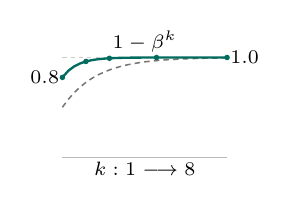
\begin{tikzpicture}[x=8.5pt,y=36pt,font=\fontsize{7}{8}\selectfont]
  % Subtle baseline and ceiling
  \draw[pdinkmuted!35,line width=.35pt] (1,0) -- (8,0);
  \draw[pdinkmuted!25,line width=.3pt,dash pattern=on 1.5pt off 1.5pt] (1,1) -- (8,1);
  % Reference curve beta=0.5 (muted dashed)
  \draw[pdinkmuted!70,line width=.55pt,dash pattern=on 2pt off 1.5pt] plot[domain=1:8,samples=29]
    (\x,{1 - 0.5^\x});
  % Primary curve beta=0.2 (solid teal)
  \draw[pdteal,line width=.85pt] plot[domain=1:8,samples=29]
    (\x,{1 - 0.2^\x});
  \foreach \k in {1,2,3,5,8}{%
    \fill[pdteal] (\k,{1 - 0.2^\k}) circle[radius=1pt];
  }
  % Labels
  \node[anchor=east,inner sep=1pt] at (1,0.8) {$0.8$};
  \node[anchor=west,inner sep=1pt] at (8,1) {$1.0$};
  \node[anchor=south,inner sep=1pt] at (4.5,1.02) {$1-\beta^k$};
  \node[anchor=north,inner sep=1.5pt] at (4.5,0) {$k: 1\longrightarrow 8$};
\end{tikzpicture}
\makeatother\endgroup
\par
\emph{Detection power:} $1-\beta^k$ as captured canary count $k$ scales ($\beta=0.2, 0.5$).} in bank bundles: each pack fails alone with probability $\beta$, so
grabbing $k$ dyed bundles fails to stain with probability $\beta^k$; how many
dyed bundles a thief grabs is set by how much he takes and how densely packs
are planted. The sequential half is quality control: each gate output is a
Bernoulli trial, and a sequential probability ratio test accumulates evidence
for ``is this stream leaking?'' The three links before this one
govern what the gate is \emph{allowed} to pass; this one measures what happens
when something tries to pass anyway. ``We have canaries'' is a mood; a security
officer buys a number. The misread to preempt: the two theorems answer two
different questions, and a single-shot exfiltration is the first theorem's job,
not the second's.

\begin{pdclaim}{Theorem}{Power}
\setlength{\parskip}{4pt plus 1pt}
\label{thm:sealed-power}
With per-canary false-negative rate $\beta$, independent across canaries, a
leak carrying $k$ canary spans is detected with probability
\[
1-\beta^k.
\]

Under\marginnote{% Analytical sparkline: Canary operating characteristic curve Pr(detect | m).
% Domain m in [0, 80] spans; p = (c/n)*(1-beta) = 0.04.
% Fits inside the 93.95pt book margin column.
% Source: thm:sealed-power operating curve.
\begingroup\makeatletter
\ifdefined\pd@typesetpicturebox
  \let\pgfsys@typesetpicturebox\pd@typesetpicturebox
\fi
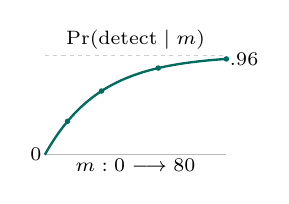
\begin{tikzpicture}[x=0.82pt,y=36pt,font=\fontsize{7}{8}\selectfont]
  % Baseline and ceiling
  \draw[pdinkmuted!35,line width=.35pt] (0,0) -- (80,0);
  \draw[pdinkmuted!25,line width=.3pt,dash pattern=on 1.5pt off 1.5pt] (0,1) -- (80,1);
  % Operating curve 1 - (1 - 0.04)^m
  \draw[pdteal,line width=.85pt] plot[domain=0:80,samples=41]
    (\x,{1 - (1 - 0.04)^\x});
  \foreach \m in {10,25,50,80}{%
    \fill[pdteal] (\m,{1 - (1 - 0.04)^\m}) circle[radius=1pt];
  }
  % Labels
  \node[anchor=east,inner sep=1pt] at (0,0) {$0$};
  \node[anchor=west,inner sep=1pt] at (80,0.96) {$.96$};
  \node[anchor=south,inner sep=1pt] at (40,1.02) {$\Pr(\text{detect}\mid m)$};
  \node[anchor=north,inner sep=1.5pt] at (40,0) {$m: 0\longrightarrow 80$};
\end{tikzpicture}
\makeatother\endgroup
\par
\emph{Operating curve:} detection probability vs.\ exfiltrated leak size $m$.} uniform planting of $c$ canaries in an $n$-span corpus, a leak of $m$ spans
chosen independently of their hidden locations
carries $K\sim\mathrm{Hypergeom}(n,c,m)$ canaries, so
\[
\Pr(\text{detect}\mid m)=1-\mathbb{E}[\beta^K]\approx
1-\bigl(1-\tfrac{c}{n}(1-\beta)\bigr)^m,
\]
the operating curve.
\end{pdclaim}

% Reserve the complete short statement, including its notation qualification.
\Needspace{18\baselineskip}
\begin{pdclaim}{Theorem}{Latency (Wald)}
\setlength{\parskip}{4pt plus 1pt}
\label{thm:sealed-latency}%
\marginnote{% Analytical sparkline: Wald sequential probability ratio test (SPRT).
% Shows upper threshold A (alarm), lower threshold B (clear), and sample trajectory.
% Fits inside the 93.95pt book margin column.
% Source: thm:sealed-latency (Wald sequential test).
\begingroup\makeatletter
\ifdefined\pd@typesetpicturebox
  \let\pgfsys@typesetpicturebox\pd@typesetpicturebox
\fi
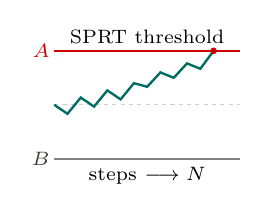
\begin{tikzpicture}[x=4.8pt,y=6.5pt,font=\fontsize{7}{8}\selectfont]
  % Upper boundary A (Alarm)
  \draw[red!80!black,line width=.65pt] (0,3) -- (14,3);
  \node[anchor=east,inner sep=1.5pt,text=red!80!black] at (0,3) {$A$};
  % Lower boundary B (Clear)
  \draw[pdinkmuted!65,line width=.65pt] (0,-3) -- (14,-3);
  \node[anchor=east,inner sep=1.5pt,text=pdinkmuted] at (0,-3) {$B$};
  % Zero line
  \draw[pdinkmuted!25,line width=.3pt,dash pattern=on 1.5pt off 1.5pt] (0,0) -- (14,0);
  % Sample cumulative log-likelihood walk reaching threshold A at step 12
  \draw[pdteal,line width=.85pt]
    (0,0) -- (1,-0.5) -- (2,0.4) -- (3,-0.1) -- (4,0.8) -- (5,0.3)
    -- (6,1.2) -- (7,1.0) -- (8,1.8) -- (9,1.5) -- (10,2.3) -- (11,2.0) -- (12,3.0);
  \fill[red!80!black] (12,3.0) circle[radius=1.2pt];
  % Labels
  \node[anchor=south,inner sep=1pt] at (7,3.2) {SPRT threshold};
  \node[anchor=north,inner sep=1.5pt] at (7,-3.2) {steps $\longrightarrow N$};
\end{tikzpicture}
\makeatother\endgroup
\par
\emph{Wald stopping boundary:} Sequential ratio walk with thresholds $A, B$.}%
Assume i.i.d. Bernoulli gate outputs under two fixed, simple hypotheses,
with rates $0<p_0<p_1<1$.

Let $L_N$ be the accumulated log-likelihood ratio
of leak to null at the uncapped SPRT's first exit from fixed thresholds,
$N$, with finite expectation.
Wald's identity gives
\[
\mathbb{E}_1[N]=\frac{\mathbb{E}_1[L_N]}{\mathrm{KL}(p_1\Vert p_0)},
\qquad
\mathbb{E}_0[N]=\frac{-\mathbb{E}_0[L_N]}{\mathrm{KL}(p_0\Vert p_1)}.
\]

Among tests with no larger \emph{actual} false-alarm and miss probabilities,
the SPRT minimizes both expected sample sizes.
\end{pdclaim}

For fixed nominal targets\pdcite{wald,wald-wolfowitz} $\alpha,\gamma>0$, $\alpha+\gamma<1$, the usual
thresholds are $A=(1-\gamma)/\alpha$ and $B=\gamma/(1-\alpha)$.
Replacing the terminal log-likelihood by $\ln A$ or $\ln B$ and the actual
error probabilities by the targets gives the \emph{no-overshoot approximation}
\[
\mathbb{E}_1[N]\approx
\frac{(1-\gamma)\ln A+\gamma\ln B}{\mathrm{KL}(p_1\Vert p_0)}.
\]
Here $\alpha$ targets false alarms; $\gamma$ targets misses and is distinct
from the per-canary miss rate $\beta$ and the
release-channel width $b$. These approximate thresholds do not separately
guarantee the two nominal error rates.

Jung, Paxson, Berger and Balakrishnan used this machinery for portscan
detection in 2004 \pdcite{jpbb04}. Their threshold random walk distinguishes
benign from scanning hosts; their analysis explicitly separates approximate
sample counts from attained errors. The canary gate borrows that statistical
question, not a guarantee that real gate outputs fit its model.

% Reserve enough height for both the short derivation and its marginal portrait.
\Needspace{14\baselineskip}
\paragraph{Proof idea.}
Power\pdmarginfigure{wald}{Wald's test decides when to stop collecting evidence.}%
\space is independence and counting: a leak is missed only if every carried
canary is missed, and the number carried under uniform planting is the
hypergeometric draw of $m$ spans from $n$ with $c$ marked. Latency is Wald's
identity: the log-likelihood ratio drifts at rate $\mathrm{KL}(p_1\Vert p_0)$
per output under the leak. The identity uses its \emph{actual terminal value},
including any boundary overshoot. It is the approximation above, not the
identity, that replaces that value by the boundary.

\paragraph{Reported checks.}
The chapter's recorded A4 example uses $n=10^4$ records with $c=100$ canaries (density
one percent), against a channel through which each smuggled canary evades the
detector with probability $\beta=0.2$: a 100-span leak is
caught with exact hypergeometric probability $0.554$, an 800-span leak at
$0.999$. The recorded conditional-power comparisons at
$k=1,2,5$ (analytic $0.800$, $0.960$, $0.99968$ against simulated $0.8016$,
$0.9608$, $0.99967$) are simulation reports, not new measurements here.
At $p_0=10^{-3}$, $p_1=10^{-2}$, $\alpha=0.01$, $\gamma=0.05$, the
no-overshoot approximations are $296.9$ outputs under leak and $431.9$ under
null; the recorded simulation means are $359.0$ and $438.1$. Reported miss
$0.048$ and false alarm $0.005$ are point estimates, not certified upper
bounds. A4's assertions permit twice the nominal error targets. Its
$200{,}000$-output cap is not reported separately: an unresolved capped run
is counted with non-upper decisions. Those records cannot establish that all
runs terminated [internal, \texttt{a4\_canary\_sprt.py}].

\begin{pdexample}{Three Canaries, One Operating Curve}
\setlength{\parskip}{4pt plus 1pt}
At $\beta=0.2$, the detection probabilities for smuggled canaries are
[verified]:
\[
\begin{aligned}
\text{two canaries:}\quad &1-0.04=0.96,\\
\text{three canaries:}\quad &1-0.008=0.992.
\end{aligned}
\]

The operating curve at $m=100$:
\[
1-(1-0.01\times0.8)^{100}=1-0.992^{100}\approx0.552
\]
by the binomial approximation, against $0.554$ exact\pdprov{a4\_canary\_sprt.py}{20260816}{internal}.

\emph{Now you try:} at the
same $\beta$, what does a five-canary leak survive with, and can you recover
the approximate $296.9$ from the formula with a pocket calculator?
(Exercises~\ref{ex:sealed-power} and \ref{ex:sealed-sprt}.)
Figure~\ref{fig:sealed-operating-curve} compares exact power, approximate
stopping counts and reported capped means.
\end{pdexample}

% Restyle of fig-sealed-operating-curve to the tikz-diagram-craft v2 standard
% (both plots are unchanged; only roles and column width are new).
%
% Reader question: how fast does detection power climb with canaries carried,
% and how long does the sequential test run?
% Claim: power climbs fast (three canaries already catch 99.2% of leaks) and
% the sequential test resolves in a few hundred outputs either way.
% Evidence: Theorem sealed-power, Theorem sealed-latency, website-v2/public/
% whitepaper/sealed-harbor.tex, Sec.~sealed-detection, "Verification" and
% "Numbers by hand" [internal, a4_canary_sprt.py].
% Must distinguish: the marked anchor (k=3, 0.992) on the power curve from
% the rest of the climb; the null run length from the leak run length.
% Grammar chosen: two-panel measured plot (pgfplots) -- power against k with
% the anchor marked, expected run length under null and leak as a bar pair.
% Grammar rejected: a single unlabeled curve would lose the worked anchor;
% a pie of outcomes has no axis for a run-length comparison.
% Five-second test: how many canaries reach 99%, and which run is longer.
% NOTE for the author: pgfplots centers `title=` on the axis without
% constraining its width, so a long bold title silently overflows the column
% independent of the axis `width=` (found via this figure: an un-constrained
% title alone pushed technical ink to 4.75in against a 6.6cm-wide axis).
% Fixed here with an explicit `text width` on `title style`; worth a QA-script
% check (figcheck T7/ink) if other pgfplots fragments carry long titles.
\begin{figure}[H]
\centering
\pdfigurehue{pdcobalt}%
\begin{tikzpicture}[pd figure]
  \begin{axis}[
    width=5.9cm,height=4.2cm,
    axis lines=left,
    title={detection power climbs fast in the number of canaries carried},
    title style={font=\pdfiglabelbold,text=pdink,yshift=-2pt,align=center,text width=5.3cm},
    xmin=0.5,xmax=8.5,ymin=0,ymax=1.05,
    xlabel={smuggled canaries $k$ (per-canary miss rate $\beta=0.2$)},
    ylabel={detection probability},
    xlabel style={font=\pdfiglabel,text=pdinkmuted,align=center,text width=5.6cm},
    ylabel style={font=\pdfiglabel,text=pdinkmuted},
    tick label style={font=\pdfiglabel,text=pdinkmuted},
    axis line style={pd hairline},
    tick style={pd tick},
    xtick={1,2,3,4,5,6,7,8},
    ytick={0,0.25,0.5,0.75,1.0},
    clip=false,
  ]
    \addplot[domain=1:8,samples=8,pd rule,mark=*,mark size=1.1pt,mark options={fill=pdink}] {1-0.2^x};
    \addplot[only marks,mark=*,mark size=1.7pt,draw=pdfocus,fill=pdfocus] coordinates {(3,0.992)};
    \draw[pd guide] (axis cs:3,0) -- (axis cs:3,0.992);
    \node[pd focus label,anchor=north west,align=left,text width=3.2cm] at (axis cs:4.4,0.62) {$k=3$: caught with probability $0.992$};
  \end{axis}
\end{tikzpicture}

\vspace{4pt}
\begin{tikzpicture}[pd figure]
  \begin{axis}[
    xbar,
    width=5.9cm,height=2.6cm,
    bar width=9pt,
    axis lines=left,
    xmin=0,xmax=520,ymin=0.4,ymax=2.6,
    ytick={1,2},
    yticklabels={{under the null},{under a leak}},
    y tick label style={font=\pdfiglabel,text=pdink,text width=2.1cm,align=right},
    xlabel={expected outputs to a stopping decision, $\mathbb{E}[N]$ (Wald)},
    xlabel style={font=\pdfiglabel,text=pdinkmuted,align=center,text width=5.6cm},
    tick label style={font=\pdfiglabel,text=pdinkmuted},
    axis line style={pd hairline},
    tick style={pd tick},
    xtick={0,100,200,300,400,500},
    clip=false,
  ]
    \addplot[pd neutral fill] coordinates {(431.9,1)};
    \addplot[pd focus fill] coordinates {(296.9,2)};
    \node[pd label,anchor=west,text=pdink] at (axis cs:436,1) {$431.9$};
    \node[pd label,anchor=west,text=pdink] at (axis cs:301,2) {$296.9$};
  \end{axis}
\end{tikzpicture}
\caption{Top: the power curve, detection probability against canaries carried, at the measured per-canary miss rate $\beta=0.2$; the chapter's anchor, three canaries caught with probability $0.992$, is marked. Bottom: the sequential test's expected run length at a null hit-rate of $0.001$, a leak hit-rate of $0.01$, a false-alarm target of $0.01$, and a miss target of $0.05$ -- Wald's formula gives $431.9$ expected outputs under the no-leak null and $296.9$ under exfiltration, idealized against a simulated overshoot of $438.1$ and $359.0$ respectively, which only helps the realized error rates.}
\label{fig:sealed-operating-curve}
\end{figure}


\paragraph{What it buys.}
Once the model is validated and the errors calibrated, a contract could
quote detection power and stopping latency under stated conditions. The exfiltration bond of
\pdchapref{bonded}{The Bonded Commons} is scoped to funding
detection and response, rather than pretending to cover unbounded breach
damage.

% Keep this short caveat whole; a deferred operating-curve float must not
% separate the single-shot qualification from its statistical-test premise.
\Needspace{12\baselineskip}
\begin{pdboundary}
\setlength{\parskip}{4pt plus 1pt}
Independence and \emph{secrecy} of planting are decisive: an adversary who
obtains the canary list with probability $0.3$ and strips all of them drops
reported simulated power from $0.9997$ to $0.698$ at $k=5$ [internal,
\texttt{a4\_canary\_sprt.py}]; canary secrecy is part of the security
boundary.

$\beta$ is a model input that requires measurement for the intended
deployment.

The nominal-target stopping-time formulas are approximations,
not certified latency or error bounds.

And
the sequential test detects \emph{statistical} leak signatures; a single-shot
exfiltration is Theorem~\ref{thm:sealed-power}'s job.
\end{pdboundary}

\section{The leakage budget: $q\cdot b$ bits, before timing}\label{sec:sealed-budget}

\begin{pdexample}{Twelve Thousand Eight Hundred Bits, and the Only Two Dials}
\setlength{\parskip}{4pt plus 1pt}
A work order grants Erin a $64$-bit status schema per job, over $200$ jobs.
Multiply, and that's the account:
\[
200\times 64=12{,}800\text{ bits}
\]
of adversarial capacity, before timing.

Two things about that arithmetic are worth a second
look, and neither needs a model. First, the account is a \emph{product}, so
the contract writer has exactly two dials and they trade off against each
other --- the same $12{,}800$ bits fall out of a narrower schema over a longer
engagement --- and the only setting that drives the product to zero is $b=0$,
which closes the feedback channel that was Erin's reason for signing in the
first place. (That is what Section~\ref{sec:sealed-limitations} means when it
says ``zero'' is available only at $b=0$; it is a price, not an impossibility.)

Second, and this is the uncomfortable half,
Theorem~\ref{thm:sealed-noninterference} does not narrow those $12{,}800$ bits
by a single one: it guarantees they left through the declared gate, not that a
worker computing $t=f(s)$ and submitting $t$ chose them innocently. The room
sells a bounded account. It does not sell an innocent one.

\emph{Now you try:}
the same work order lets each job return at one of three scheduled times ---
what does that add to the total? (Exercise~\ref{ex:sealed-budget}.)
\end{pdexample}

The four links compose into one information-theoretic account, and the account
is deliberately unromantic. It is also where the chapter pays three debts it
took on earlier: the laundering residual left open by
Theorem~\ref{thm:sealed-noninterference}'s committed-input hypothesis, the
malicious worker for whom $\sigma\le\varepsilon_{\max}$ does not certify differential privacy,
and the arbitrary-telemetry channel disclaimed in
Section~\ref{sec:sealed-limitations}. All three are the same debt seen from
three sides, and it has one price, drawn converging in
Figure~\ref{fig:sealed-residuals-converge}.

% Fragment: fig-sealed-residuals-converge.tex -- three residuals opened
% earlier in the chapter, one q*b account that prices all of them.
%
% Reader question: why do three separate gaps opened earlier in the
% chapter all get paid off by one number?
% Claim: the laundering residual, the malicious-worker gap in the ledger,
% and the arbitrary-telemetry channel are three faces of one debt, all
% priced by the same q*b capacity account -- not three independent
% problems needing three independent fixes.
% Evidence: opening paragraph of Sec. sealed-budget, website-v2/public/
% whitepaper/sealed-harbor.tex ("It is also where the chapter pays three
% debts it took on earlier: the laundering residual...the malicious
% worker...and the arbitrary-telemetry channel...All three are the same
% debt seen from three sides, and it has one price.").
% Must distinguish: three DIFFERENT sources (different sections, different
% failure shapes) from one SHARED sink -- the figure must not suggest
% three separate accounts that happen to look similar; there is exactly
% one q*b bucket, filled from three pipes.
% Grammar chosen: converging pipes into one bucket (S12's ledger
% convention: asset pools are buckets joined by directed pipes) -- reused
% here as three named residuals piping into the one leakage-budget bucket
% introduced in fig-sealed-leakage-ledger, this row's own paired panel.
% Grammar rejected: three separate small ledgers, one per residual --
% that is the "three independent problems" misreading the chapter is
% explicit about ruling out.
% Five-second test: count the buckets -- one, fed by three pipes, not
% three buckets side by side.
% QA: beauty_lint warns B7 in all three editions (sub-point
% near-alignment noise among the three stacked source nodes' centres);
% justified, not fixed.
\begin{figure}[H]
\centering
\pdfigurehue{pdcobalt}%
\begin{tikzpicture}[pd figure,x=1cm,y=1cm]
  % The explicit box leaves print-size air above the heavy first node. Without
  % it, fragment cropping trims to that node's inferred top rule.
  \path[use as bounding box] (-0.35,-1.35) rectangle (9.25,4.95);
  \def\dy{1.85}
  \node[pd title,anchor=south west] at (-0.10,4.45)
    {three residuals, one account};
  \node[pd breach state,minimum width=4.1cm,align=center] (R1) at (0,{2*\dy})
    {laundering residual\\\pdfigsub worker computes $t=f(s)$};
  \node[pd breach state,minimum width=4.1cm,align=center] (R2) at (0,{1*\dy})
    {malicious worker\\\pdfigsub declares its own $\varepsilon_i$};
  \node[pd breach state,minimum width=4.1cm,align=center] (R3) at (0,0)
    {arbitrary telemetry\\\pdfigsub unconstrained prose channel};
  \node[pd bucket,minimum width=3.0cm,minimum height=2.4cm,align=center]
    (ACCT) at (6.5,{1*\dy}) {\\[8pt]the $q\cdot b$\\account};
  \draw[pd focus pipe] (R1.east) -| (ACCT.north);
  \draw[pd focus pipe] (R2.east) -- (ACCT.west);
  \draw[pd focus pipe] (R3.east) -| (ACCT.south);
\end{tikzpicture}
\caption{Three named residuals converge on one leakage-capacity account. Each
lets the worker choose bits that the noninterference property does not forbid,
so all three are priced by the same $q\cdot b$ bound rather than by separate
mechanisms. [internal]}
\label{fig:sealed-residuals-converge}
\end{figure}

% The following capacity/timing explanation must follow its exhibit, rather
% than start before a deferred figure and resume beneath it on the next page.
\FloatBarrier

\pdmarginanalogy{sealed-lead-darkslide}{}{ch03-lead-lined-darkslide}{Like a photographic plate holder with a lead darkslide shielding stray radiation, a zero-knowledge attestation exposes validity without revealing underlying confidential data.}%
If an Erin-visible channel permits $b$
freely chosen bits per job, a malicious worker, one that launders by computing
$t=f(s)$ and submitting $t$ so that the gate honestly releases $g(t)$, can
exfiltrate up to $b$ bits through it: the noninterference property guarantees
only that those bits pass through the declared gate, not that they are
innocent. Across $q$ jobs the raw capacity is $q\cdot b$ bits; choosing among
$s$ timing slots adds up to $\log_2 s$ bits per event, which is why timing sits
outside the possibilistic model. The $\log_2 s$ expression is a finite-alphabet
upper bound: across at most $q$ events, at most $s^q$ slot sequences are
distinguishable. Predictive mitigation \pdcite{azm10} provides a framework for
controlling timing observations; the slot count here is not a proof for an
arbitrary scheduler.

The observation model matters. Infinite timing precision can admit unbounded
information in an idealized duration, but practical capacity also depends on
clock resolution, noise, observation windows, and bandwidth. A bucketed-release
design must account for aborts, missed slots, termination, and the number of
events. If those vary with secrets and remain visible, quantizing successful
releases alone leaves a channel open. Fixed deadlines and padded outcomes,
including failure and no-result cases, are additional design obligations.

Finite output alphabets and query limits can bound specified observations;
they do not bound every host side channel. Nor are bit budgets interchangeable
with differential-privacy parameters: the latter require the mechanism and
adjacency assumptions of Section~\ref{sec:sealed-conservation}. Canaries provide
probabilistic detection evidence, not exhaustive policing of the allowed
capacity. Contracts may price residual risk, but neither the price nor a clean
canary run proves that semantic laundering did not occur.

% Book redraw: VIII/fig:sealed-leakage-ledger.
% Source-derived conceptual capacity accounting; no fresh experiment, proof, model,
% provider, runtime, or deployment evidence is claimed.
% Owner boundary: website-v2/public/whitepaper/sealed-harbor.tex,
% sec:sealed-budget. Two-row accounting flow feeding a single visible capacity
% ledger account, distinguishing fixed status capacity from discrete timing capacity.
\begin{figure}[H]
\centering
\SGMeasuredFigure{VIII/fig:sealed-leakage-ledger}{%
\begin{tikzpicture}[sg/base]
  % Native canvas: 316pt wide, comfortably below the 325.215pt Book column.
  % Two contract lanes route into one transparent, auditable Swiss capacity ledger.
  \path[draw=sgGrid,line width=.35pt] (0,0)--(180,0);
  \path[draw=sgGrid,line width=.35pt] (0,71)--(180,71);
  \path[draw=sgGrid,line width=.35pt] (0,142)--(180,142);

  % --- Lane 1: Fixed status channel (top) --------------------------------
  % Folded contract document representing fixed payload agreement
  \draw[draw=sgInk,fill=sgBlue!6,line width=.75pt]
    (8,80)--(54,80)--(62,88)--(62,130)--(8,130)--cycle;
  \draw[sgInk,line width=.6pt] (54,80)--(54,88)--(62,88);
  \node[font=\SGType\bfseries,text=sgBlue,align=center] at (35,114)
    {status\\terms};
  \node[font=\SGType,text=sgInk,align=center] at (35,94)
    {200 jobs\\$\times$ 64 bits};

  \draw[sgBlue,line width=1.35pt] (70,128)--(176,128);
  \node[anchor=west,font=\SGType\bfseries,text=sgBlue] at (70,121)
    {fixed status channel};
  \node[anchor=north west,font=\SGType,align=left] at (70,118)
    {$200 \times 64 = \mathbf{12{,}800\text{ bits}}$};
  \node[anchor=north west,font=\SGType,text=sgInk!70,align=left] at (70,102)
    {declared payload bits};
  \draw[sg/arrow] (178,105)--(204,105)--(216,88)--(226,88);

  % --- Lane 2: Discrete timing channel (bottom) --------------------------
  % Folded contract document representing scheduled timing agreement
  \draw[draw=sgInk,fill=sgAmber!8,line width=.75pt]
    (8,12)--(54,12)--(62,20)--(62,62)--(8,62)--cycle;
  \draw[sgInk,line width=.6pt] (54,12)--(54,20)--(62,20);
  \node[font=\SGType\bfseries,text=sgAmber,align=center] at (35,46)
    {timing\\terms};
  \node[font=\SGType,text=sgInk,align=center] at (35,26)
    {200 returns\\$\times \log_2(3)$};

  \draw[sgAmber,line width=1.35pt] (70,60)--(176,60);
  \node[anchor=west,font=\SGType\bfseries,text=sgAmber] at (70,53)
    {scheduled timing slots};
  \node[anchor=north west,font=\SGType,align=left] at (70,50)
    {$200 \times 1.585 \approx \mathbf{+317\text{ bits}}$};
  \node[anchor=north west,font=\SGType,text=sgInk!70,align=left] at (70,34)
    {3 return horizons};
  \draw[sg/arrow] (178,37)--(204,37)--(216,54)--(226,54);

  % --- Destination: Swiss capacity ledger balance -----------------------
  % Clean accounting card matching Figure 3.13's envelope grammar
  \draw[draw=sgInk,fill=sgTeal!6,line width=.85pt]
    (226,10) rectangle (316,134);
  \draw[sgTeal,line width=1.6pt] (226,134)--(316,134);
  \node[font=\SGType\bfseries,text=sgTeal,align=center] at (271,122)
    {capacity ledger};
  \node[font=\SGType,text=sgInk!75,align=center] at (271,110)
    {one contract balance};
  \draw[sgGrid,line width=.5pt] (232,102)--(310,102);

  \node[anchor=west,font=\SGType,text=sgInk] at (232,88) {status:};
  \node[anchor=east,font=\SGType\bfseries,text=sgBlue] at (310,88) {12{,}800};
  \node[anchor=west,font=\SGType,text=sgInk] at (232,68) {timing:};
  \node[anchor=east,font=\SGType\bfseries,text=sgAmber] at (310,68) {$+317$};

  % Accounting rule and balanced sum
  \draw[sgInk,line width=.65pt] (232,54)--(310,54);
  \node[anchor=west,font=\SGType\bfseries,text=sgInk] at (232,40) {total:};
  \node[anchor=east,font=\SGType\bfseries,text=sgTeal] at (310,40) {\textbf{13{,}117}};
  \draw[sgTeal,line width=.85pt] (232,29)--(310,29);
  \draw[sgTeal,line width=.85pt] (232,26)--(310,26);
  \node[font=\SGType,text=sgInk!75,align=center] at (271,17)
    {bits of capacity};
\end{tikzpicture}}
\caption{For 200 jobs, fixed status plus three return slots yields about 13,117 bits of adversarial capacity. The capacity ledger accounts for both explicit payloads and discrete timing horizons without conflating their channels. [hand-derived; Exercise~\ref{ex:sealed-budget}]}
\label{fig:sealed-leakage-ledger}
\end{figure}


\section{Limitations and boundaries}\label{sec:sealed-limitations}

None of the following is promised, and a contract that implies any of them
overclaims.

Table~\ref{tab:sealed-not-promised} lists six of them: for each, what
mechanism is responsible for the gap, and where -- if anywhere -- the residual
is priced.

\begin{table}[H]\centering\footnotesize
\caption{Six things this design does not promise, why not, and where the
residual is priced. A contract that implies any of these overclaims.}
\label{tab:sealed-not-promised}
\begin{tabularx}{\textwidth}{@{}>{\raggedright\arraybackslash}p{3.5cm} >{\raggedright\arraybackslash}X >{\raggedright\arraybackslash}p{3.3cm}@{}}
\toprule
Not promised & Why not & Residual priced by \\
\midrule
Zero model leakage under unlimited adaptive queries to Derek & Derek \emph{intentionally observes} evaluations of $M$; unlimited black-box access enables model extraction & out of model: bounded only by the contracted query-and-output interface \\
Zero data leakage with arbitrary natural-language telemetry to Erin & that channel is exactly the $q\cdot b$ budget; ``zero'' needs $b=0$ & the $q\cdot b$ budget (Sec.~\ref{sec:sealed-budget}) \\
Elimination of timing, cache, speculative, firmware, or physical channels & the noninterference guarantee is possibilistic & out of model; padded and scheduled, not closed \\
Confidentiality through an unapproved external model or tool provider & a remote API that reads plaintext is another trusted reader & not priced: the model must run inside the confidential domain, or the guarantee does not apply \\
Correctness of the answer & the receipt proves what the measured system reported, not that it is true & out of model \\
Literal deletion of information already observed, availability under refusal, or collusion resistance & each needs a strictly stronger threat model & needs MPC or homomorphic backends, not priced here \\
\bottomrule
\end{tabularx}
\end{table}

% Keep this limitations table before the following extension/proof discussion.
\FloatBarrier
One more limit sits outside even that table: bounds on minds. A human who
reads a released aggregate may still remember it; the system bounds
channels, not memories.

\paragraph{The lift.}
Theorem~\ref{thm:sealed-noninterference} is exhaustive on a finite model; the
general claim over unbounded state is a proof obligation with a known shape.
Rushby's channel-control formulation \pdcite{rushby} reduces noninterference for
a transition system to three local \emph{unwinding conditions}, output
consistency, step consistency, and local respect, each a per-transition lemma
amenable to mechanization, and the Isabelle Archive of Formal Proofs already
carries stateful intransitive-noninterference developments in exactly this
lineage. The finite model is the blueprint: its local-respect check already
holds mechanically, its declassification steps are the intransitive
downgrader domain of Rushby's framework, and the lift consists of restating the
transition relation abstractly and discharging the three lemmas once, for all
depths and all secrets. One precision the lift must get right from the start:
Rushby's soundness result for these conditions is with respect to intransitive
purge, but van der Meyden shows the conditions are sound \emph{and complete}
for the strictly stronger TA-security property, which additionally preserves
the \emph{order} of permitted transmissions \pdcite{vdm07}. Discharging the
three lemmas therefore certifies TA-security, and the lift should state that
target explicitly. Two extensions of the finite model are open alongside the
lift: a \texttt{submit} that carries a payload, so the mutation suite can
exhibit laundering, and a partial-observation variant of the enforceability
check for policies that reference unmediated state. The status of every claim
in this chapter is: the two exhaustive checks are \pdassurance{Attested} on
their scripts; the canary simulation values are chapter-reported, without an
archival run receipt or calibrated error bounds supplied here. The room itself is a
\pdassurance{Confined} design whose complete-mediation invariant is attested
per deployment, not proved.

\pdexercisepointer*{\ref{ex:sealed-pairs}}{\ref{ex:sealed-budget}}{\pageref{ex:sealed-pairs}}
\begin{pdrecitation}
\item Without looking: state the sentence that replaces ``mathematically cannot
  phone home,'' and name the theorem that makes each of its three adjectives
  true.
\item Which link must hold before the conservation theorem says anything about
  the deployment, and why?
\item A contract grants a 32-bit status per job over 400 jobs. What is the
  adversarial capacity before timing, and which link polices it?
\end{pdrecitation}


\section*{Review of the key ideas}
\addcontentsline{toc}{section}{Review of the key ideas}
What this chapter leaves coupled, in the order the rest of the book will lean on it:

\begin{enumerate}[leftmargin=1.6em,itemsep=2pt]
\item A \textbf{sealed room} lets an agent compute on data it may not export: the data owner and the model owner each get their guarantee from a fence they can inspect, not from trust in the other.
\item \textbf{Taint does not survive a language model.} Token-level information flow through the model is not soundly definable, so the room does not try; it fences the room and gates the slot.
\item \textbf{Two fences, two gates}: the work order fixes what may enter, the slot fixes what may leave, and the model in between is treated as an opaque function of both.
\item \textbf{Noninterference is checked by running the world twice} (self-composition, in the verification literature's word): identical except for the secret, the two runs must agree on everything that leaves through the slot, modulo the declassification the gate performs. The finite clean-room model passes this check to depth seven.
\item The gate sits on the \textbf{only enforceable boundary}: a policy over the agent's behavior is enforceable exactly when its trigger is witnessed at the slot; anything decided inside the room is detect-only.
\item \textbf{The privacy budget is a ledger that conserves}: every release debits $\varepsilon$, the ledger's total never exceeds $\varepsilon_{\max}$, and a torn write is caught by the invariant within three steps on the two-client instance.
\item \textbf{Canaries have conditional power}: a leak carrying $k$ canaries escapes all their independent detections with probability $\beta^{k}$ ($0.008$ at $\beta=0.2$, $k=3$). The sequential model estimates outputs until either decision, not a guaranteed alarm deadline.
\item The whole channel is priced before timing: \textbf{$q \cdot b$ bits} may leave through $q$ queries of $b$ bits each, and the room's guarantee is that budget, not silence.
\end{enumerate}

\section{Exercises}
\label{sec:sealed-exercises}

\pdexercisesfor{\S\ref{sec:sealed-limitations}}{Limitations and boundaries}

\begin{pdexercise}[kind=Check,rating=1]{ex:sealed-pairs}
With $g(s)=s\bmod 2$ over secrets $\{0,\dots,7\}$, how many unordered secret
pairs must a sound room keep Erin-indistinguishable, and how many may differ at
release steps?
\end{pdexercise}
\begin{pdsolution}{ex:sealed-pairs}
Both parity classes have four members, so the equal-parity pairs number
$2\binom{4}{2}=12$; those must stay indistinguishable forever. The remaining
$\binom{8}{2}-12=16$ pairs have different parities and may differ at explicit
gate-release steps only. Table~\ref{tab:sealed-parity-pairs} shows how this
scales: doubling the secret count roughly quadruples both counts, since
both grow quadratically in $n$ while the equal-parity share of the total
stays fixed at one half.
\end{pdsolution}

\begin{table}[H]\centering\footnotesize
\caption{For $g(s)=s\bmod 2$, equal-parity pairs stay hidden; different-parity
pairs may differ only at release.}
\label{tab:sealed-parity-pairs}
\begin{tabularx}{\textwidth}{@{}c >{\centering\arraybackslash}X >{\centering\arraybackslash}X >{\centering\arraybackslash}X@{}}
\toprule
Secrets & Unordered pairs & Equal parity & Different parity \\
\midrule
4 & $\binom{4}{2}=6$ & 2 & 4 \\
8 & $\binom{8}{2}=28$ & 12 & 16 \\
\bottomrule
\end{tabularx}
\end{table}

\begin{pdexercise}[kind=Trace,rating=2]{ex:sealed-m1-trace}
Run \texttt{c1\_noninterference.py} and read the first mutation's witness. Why
is the decisive pair $(0,2)$ rather than $(0,1)$, and at which step of the
four does Erin's view first differ?
\end{pdexercise}
\begin{pdsolution}{ex:sealed-m1-trace}
The script prints
\begin{quote}\footnotesize\texttt{[m1 leaky gate: releases raw s] caught: EQUAL-CLASS VIOLATION}\\
\texttt{witness: secrets (0,2), trace load\_data -> read\_secret ->}\\
\texttt{submit\_to\_gate -> gate\_release, Erin sees (('gate', 0),) vs (('gate', 2),)}
\end{quote}
The pair $(0,1)$ has different parities, so the honest gate is
\emph{allowed} to let Erin's view differ at a release step; a difference there
proves nothing. The pair $(0,2)$ has equal parity, so any difference is a
violation, and it appears at the fourth step, the release, when the leaky gate
emits the raw secret instead of its parity.
\end{pdsolution}

\begin{pdexercise}[kind=Check,rating=1]{ex:sealed-bypass}
The second mutation is caught in three steps. Which side property of
Design invariant~\ref{inv:sealed-side} does the mutant violate, and why is that
violation detectable by the two-run check at all?
\end{pdexercise}
\begin{pdsolution}{ex:sealed-bypass}
The witness is \texttt{load\_data -> read\_secret -> BYPASS\_write\_E}, with
Erin seeing \texttt{(('leak', 0),)} against \texttt{(('leak', 1),)}: complete
mediation fails, since a release occurred with no gate decision. The two-run
check sees it because the bypass write lands in Erin-observable state at a step
that is not a gate release, which is a difference the property forbids for
every pair, whatever their parity.
\end{pdsolution}

\begin{pdexercise}[kind=Open,rating=3]{ex:sealed-launder}
Extend the finite model so that \texttt{submit} carries a payload the worker
computes from the secret, and state what the checker would then have to
quantify over to exhibit the laundering attack. Why is the delimited-release
remedy, enforcement at the point of declassification, unavailable for a
language-model worker?
\end{pdexercise}
\begin{pdsolution}{ex:sealed-launder}
Add a worker register $t$, a transition $\mathtt{compute}(f)$ that sets
$t=f(s)$ for $f$ drawn from a finite family, and let \texttt{submit} pass $t$
to the gate, which releases $g(t)$. The property must then be stated over
worlds that agree on $g(s)$ but may disagree on $g(f(s))$, and the checker must
quantify over the family of $f$; for any non-constant $f$ that maps an
equal-parity pair to a different-parity pair, the honest gate releases a
difference and the attack is exhibited. Delimited release rules the attack out
by requiring that no variable used in a declassification is updated before it,
which a compiler can check because the declassified expression is syntactic.
A language model's release candidate is arbitrary output, not an expression
the checker can identify, so the condition cannot be enforced and the residual
is priced as channel capacity instead.
\end{pdsolution}

\begin{pdexercise}[kind=Check,rating=1]{ex:sealed-compound}
Using the controllability theorem of \pdchapref{swk}{The Single-Writer Kernel},
explain in two sentences why ``no \texttt{net\_egress} after an
\texttt{in\_context\_read} of a secret'' is regimentable but ``no
\texttt{in\_context\_read} of a secret'' is not.
\end{pdexercise}
\begin{pdsolution}{ex:sealed-compound}
The compound rule disables only \texttt{net\_egress}, a controllable event, in
the tainted state, and never disables the uncontrollable read, so its closed
loop is controllable and a supervisor realises it exactly. The second rule
must disable \texttt{in\_context\_read} itself, an event in $\Sigma_u$ that the
plant enables, so controllability fails on the first history that reads and the
rule is detect-only.
\end{pdsolution}

\begin{pdexercise}[kind=Trace,rating=2]{ex:sealed-torn}
Reconstruct by hand the three-step torn-write crime on the two-client instance
(programs $(2,2)$ and $(1,2)$, $\varepsilon_{\max}=4$): give the sequence of
releases, the balance $\sigma$ after each, and the recorded sum
$\sum_\Lambda$, and show where the recorded sum exceeds the maximum.
\end{pdexercise}
\begin{pdsolution}{ex:sealed-torn}
Under the torn write each release logs $\varepsilon$ but adds $\varepsilon-1$.
Client 0 releases 2: log 2, $\sigma=1$, $\sum_\Lambda=2$. Client 0 releases 2
again: the guard sees $\sigma+2=3\le4$ and admits it; log 2, $\sigma=2$,
$\sum_\Lambda=4$. Client 1 releases 1: the guard sees $\sigma+1=3\le4$ and
admits it; log 1, $\sigma=2$, $\sum_\Lambda=5>4$. The script prints exactly
this trace:
\begin{quote}\footnotesize\texttt{c0.release(2) [TORN: log 2, sigma +1] ->}\\
\texttt{c0.release(2) [TORN: log 2, sigma +1] -> c1.release(1) [TORN: log 1, sigma +0]}
\end{quote}
The balance never breaks the bound, so the guard keeps admitting, and the
auditable log overspends.
\end{pdsolution}

\begin{pdexercise}[kind=Trace,rating=2]{ex:sealed-15-states}
The checked instance has 15 reachable states but only 11 distinct multisets of
committed releases. Explain the difference and exhibit two states that share a
multiset.
\end{pdexercise}
\begin{pdsolution}{ex:sealed-15-states}
A denied release still advances the denying client's program counter, so the
state records not only what was committed but which requests have already been
refused. Two interleavings that commit the same releases but differ in whether
a client's later request has already been refused are distinct states with the
same multiset. For example, after client 0 commits both of its releases
($\sigma=4$), the state before client 1's first request is refused and the
state after it is refused carry the same ledger $\{2,2\}$ and different
counters.
\end{pdsolution}

\begin{pdexercise}[kind=Check,rating=1]{ex:sealed-crossover}
At $\delta'=10^{-6}$: which bound is smaller at $k=8$, $\varepsilon=0.5$? And at
$\varepsilon=0.1$, what is the smallest $k$ at which the advanced bound falls
below basic composition?
\end{pdexercise}
\begin{pdsolution}{ex:sealed-crossover}
At $k=8$, $\varepsilon=0.5$: basic $4.00$; advanced
$\sqrt{16\ln 10^{6}}\times0.5+8\times0.5\times(e^{0.5}-1)=7.43+2.59=10.03$,
so quote the sequential bound, by a wide margin [verified]. At
$\varepsilon=0.1$ the advanced bound is
$0.1\sqrt{2k\ln 10^{6}}+0.010517k$; at $k=34$ it is $3.42$ against basic
$3.40$, and at $k=35$ it is $3.48$ against $3.50$, so the crossover is $k=35$
[verified].
\end{pdsolution}

\begin{pdexercise}[kind=Check,rating=1]{ex:sealed-power}
At $\beta=0.2$, with what probability does a five-canary leak survive
undetected? Then use the binomial approximation of the operating curve at
$n=10^4$, $c=100$, $m=100$ and compare with the exact value $0.554$.
\end{pdexercise}
\begin{pdsolution}{ex:sealed-power}
$\beta^5=0.00032$, so detection is $0.99968$ [verified]; the script's analytic
line reads \texttt{k=5: analytic 0.99968 simulated 0.99967}. The approximation
gives $1-(1-0.01\times0.8)^{100}=1-0.992^{100}\approx0.552$.
The exact hypergeometric probability is approximately $0.554$; before rounding,
the approximation is lower by about $0.00143$\pdprov{a4\_canary\_sprt.py}{20260816}{internal}.
\end{pdsolution}

\begin{pdexercise}[kind=Trace,rating=2]{ex:sealed-sprt}
Recover the no-overshoot approximation, $\mathbb{E}_1[N]\approx296.9$, following
Theorem~\ref{thm:sealed-latency} at $p_0=10^{-3}$, $p_1=10^{-2}$,
$\alpha=0.01$, $\gamma=0.05$. Why need the reported simulation mean of $359$
not equal it, and why is neither number a guaranteed alarm deadline?
\end{pdexercise}
\begin{pdsolution}{ex:sealed-sprt}
% Keep the calculation and its essential statistical qualifications together.
\interlinepenalty=10000\relax
$\mathrm{KL}(p_1\Vert p_0)=0.01\ln10+0.99\ln(0.99/0.999)\approx0.01407$.
The numerator is $0.95\ln95+0.05\ln(0.05/0.99)\approx4.177$;
their quotient is $296.9$ [verified arithmetic]. Boundary values replace terminal
log-likelihoods; nominal targets replace attained errors. Overshoot, sampling
uncertainty and the cap can affect the reported $359$, a capped sample mean, not an
exact expectation. Non-detection
$0.0483$ and false alarm $0.0052$ are point estimates, not upper bounds.
Stopping counts include either decision; no wall-clock arrival model is specified.
\end{pdsolution}

\begin{pdexercise}[kind=Open,rating=3]{ex:sealed-canary-secrecy}
An adversary obtains the canary list with probability $0.3$ and strips every
canary it knows. Reported simulated power at $k=5$ falls from $0.9997$ to $0.698$.
Propose one contract clause and one mechanism change that restore most of the
lost power, and say what no redesign can restore.
\end{pdexercise}
\begin{pdsolution}{ex:sealed-canary-secrecy}
The clause: canary secrecy is a named security boundary, so disclosure of the
planting list is a breach with its own bond, and the list is regenerated per
job. The mechanism: plant per job from a fresh seed held by Derek's gateway
alone, so a stolen list has value for one job only and the compromise
probability applies per job rather than per engagement; power then returns
toward $1-\beta^k$ for every job whose list was not taken. What no redesign
restores is power against an adversary who holds \emph{this} job's list: with
the canaries stripped the leak carries none and Theorem~\ref{thm:sealed-power}
gives $1-\beta^0=0$, which is why detection is priced as a bounded bond and not
sold as a guarantee.
\end{pdsolution}

% Keep this compact question together; its timing qualifier is part of the task.
\Needspace{7\baselineskip}
\begin{pdexercise}[kind=Check,rating=1]{ex:sealed-budget}
A work order grants Erin a 64-bit status schema per job over 200 jobs, and each
job may return at one of three scheduled times. What adversarial capacity has
the contract granted, before and after timing?
\end{pdexercise}
\begin{pdsolution}{ex:sealed-budget}
Before timing, $q\cdot b=200\times64=12{,}800$ bits. Three timing slots add up
to $\log_2 3\approx1.585$ bits per job, so about $317$ more bits, for roughly
$13{,}117$ bits in total; the timing term is why scheduled release with one
slot is the design default.
\end{pdsolution}

\section{History and references}
\label{sec:sealed-history}

Almost nothing in this chapter is new machinery; what is new is which pieces
were bolted to which, and the honest accounting of what the bolted-together
thing does not promise. It is worth saying where each piece came from.

\paragraph{Noninterference and its proof technique.}
Noninterference is Goguen and Meseguer's, stated at Oakland in 1982 as a
property of a security \emph{model} rather than of any particular mechanism
\pdcite{goguen-meseguer-82}, and given two years later the proof technique that
made it usable: replace the quantification over all runs with local
\emph{unwinding} conditions you can discharge one transition at a time
\pdcite{goguen-meseguer-84}. Rushby's 1992 report is the version this chapter
actually leans on, because it separates transitive from intransitive policies
--- which is precisely what allows a room to have a declassifier and still have
a theorem --- and because it fixes the three unwinding conditions, output
consistency, step consistency and local respect, that
Section~\ref{sec:sealed-limitations} names as the lift's proof obligation
\pdcite{rushby}. Van der Meyden later showed those conditions are not merely
sound but sound \emph{and} complete, and for the strictly stronger,
order-preserving TA-security rather than for the intransitive purge Rushby was
aiming at \pdcite{vdm07}; that is why the lift should be written to claim
TA-security rather than to settle for what it was pointed at. The checking
move itself, running the world twice and stating an ordinary invariant about
the pair, is self-composition, published by Barthe, D'Argenio and Rezk in 2004
\pdcite{bdr04}; they apply it to programs with a logic, this chapter applies it
to a finite model with a Python script, and the difference in ambition should
not obscure that it is the same move.

\paragraph{Declassification, and why the room needs the word.}
That an information-flow certifier faces a choice between label creep and
unsoundness is the oldest result in this lineage, from the Dennings'
certification lattice \pdcite{denning77}, with the modern restatement --- a
sound purely dynamic monitor must be strictly more restrictive than a static
analysis --- due to Russo and Sabelfeld \pdcite{rs10}. The escape hatch itself
is Sabelfeld and Myers's delimited release \pdcite{sm03}, and so, importantly,
is the laundering attack this chapter cannot rule out: they named it and closed
it by enforcement, requiring that no variable used in a declassification be
updated before it, which a compiler can check because the declassified
expression is syntax. This chapter's worker emits arbitrary prose rather than
an expression, so the remedy is unavailable and the residual is priced instead
--- that substitution, enforcement traded for a capacity account, is the
chapter's own move and its own liability. The vocabulary for saying which
dimension of release a mechanism actually controls is Sabelfeld and Sands's
\pdcite{ss09}; by their taxonomy the release ledger answers \emph{what},
\emph{who} and \emph{where}, and leaves \emph{when} open. Owner-indexed labels
under mutual distrust, which is the shape of the four-state lattice counted in
Section~\ref{sec:sealed-design}, are Myers and Liskov's decentralized label
model \pdcite{myers-liskov}.

\paragraph{The monitor, and the boundary it can hold.}
The in-guest monitor and Derek's outer gateway are a reference monitor in
Anderson's 1972 sense --- always invoked, tamper-resistant, small enough to be
examined \pdcite{anderson1972} --- enforcing the sort of owner-indexed access
structure Lampson's \emph{Protection} gave operating systems two years later
\pdcite{lampson1974}. What this chapter adds to that inheritance is not a
better monitor but a sharper statement of where a monitor can be placed at all:
the controllability result is proved in \pdchapref{swk}{The Single-Writer
Kernel} and merely applied here, and the caveat that partial observation
shrinks the enforceable set is Lin and Wonham's \pdcite{lin-wonham}. The
confinement architecture has a direct systems ancestor in Ryoan
\pdcite{ryoan16}, which solved the two-suspicious-owners problem first and
solved it more cleanly than this chapter does, at the price of a stateless
module; the dual-attested key release follows the attester/verifier/relying-party
pattern the IETF later standardized \pdcite{rats}.

\paragraph{Pricing what does cross.}
Treating leakage as a quantity rather than a predicate is quantitative
information flow, and the min-entropy formulation the chapter borrows its
vocabulary from is Smith's \pdcite{smith-qif}; the bridge between that currency
and differential privacy's exists, due to Alvim and colleagues
\pdcite{aacp11}, and this chapter does not cross it, which is why it carries
two accounts rather than one. On the privacy side, advanced composition is
Dwork, Rothblum and Vadhan's \pdcite{drv}; the observation that a running
budget needs a different theorem when privacy parameters and the stopping point
are chosen adaptively, and the odometer/filter pair that supplies it, is Rogers,
Roth, Ullman and Vadhan's \pdcite{rruv16}; the fully adaptive filter that
matches advanced-composition rates and leading constants is Whitehouse and colleagues'
\pdcite{wrrw23}. That production budget schedulers assume a trusted analyst,
an assumption this chapter explicitly declines about Erin's worker, is visible
in the Privacy Budget Scheduling work \pdcite{pkube21}. The detector is Wald's
sequential probability ratio test \pdcite{wald}, optimal against tests with
no larger attained errors under the simple i.i.d. hypotheses, as he and
Wolfowitz proved three years later \pdcite{wald-wolfowitz}; pointing it at a
security stream is not new either, since Jung, Paxson, Berger and Balakrishnan
did so for portscan detection in 2004 \pdcite{jpbb04}. The canary gate borrows
the comparison, subject to validating its own statistical model.

\paragraph{What is this chapter's own, and therefore uncited.}
Four things. Hypothesis~\ref{hyp:sealed-taint}, that token-level taint through
a generative model is not soundly definable, is a design rationale and not a
theorem: it rests on the Denning and Russo--Sabelfeld results above, but no
published result states it for generative models, so the chapter states it as
its own position and places the burden of a counterexample on whoever wants
one. The four-link composition read as an \emph{evidence schedule} rather than
as four redundant guarantees is the chapter's framing. The $q\cdot b$ account
as the explicit price of the laundering residual --- the thing the
noninterference theorem leaves open and delimited release would have closed by
enforcement --- is the chapter's own construction, and so is the design rule it
yields, that one should never negotiate over whether an output contains a
secret and always over channel capacity. And the ``clean room'' of the
framing is borrowed from industrial and legal practice for its connotation
only; this chapter claims no formal ancestor for the metaphor and proves
nothing about it as such.

\paragraph{Further reading.}
A reader who wants the general theorem this chapter's finite model stands in
for should read Rushby \pdcite{rushby} and then van der Meyden
\pdcite{vdm07} in that order, and should expect the second to change what the
first looks like it was proving. A reader who wants to know why the assurance
ladder in Section~\ref{sec:sealed-enforceability} is a third axis rather than a
rebadging of two familiar ones should read Sheridan and Verplank
\pdcite{sheridanverplank1978} and its four-stage refinement
\pdcite{parasuraman2000} for the automation-level axis, and the Common
Criteria's evaluation assurance levels \pdcite{cciso15408} for the
evaluation-effort axis; neither answers which component's failure would
falsify a given runtime record, which is the only question the ladder asks.

\pdprintsolutions

\begin{thebibliography}{99}

\bibitem{goguen-meseguer-82} J.~A. Goguen and J.~Meseguer. Security policies and security models. In
\emph{Proc.\ IEEE Symposium on Security and Privacy (Oakland)}, pp.~11--20, 1982.

\bibitem{goguen-meseguer-84} J.~A. Goguen and J.~Meseguer. Unwinding and inference control. In
\emph{Proc.\ IEEE Symposium on Security and Privacy}, 1984.

\bibitem{rushby} J.~Rushby. Noninterference, transitivity, and channel-control security policies.
Technical Report CSL-92-02, SRI International, December 1992.

\bibitem{vdm07} R.~van der Meyden. What, indeed, is intransitive noninterference? (extended abstract). In
\emph{Proc.\ European Symposium on Research in Computer Security (ESORICS)}, LNCS 4734, pages 235--250, 2007.

\bibitem{lin-wonham} F.~Lin and W.~M. Wonham. On observability of discrete-event systems.
\emph{Information Sciences}, 44(3):173--198, 1988.

\bibitem{anderson1972} James P. Anderson. Computer Security Technology Planning Study.
ESD-TR-73-51, U.S. Air Force Electronic Systems Division, 1972. (The origin of the
\emph{reference monitor} concept.)

\bibitem{lampson1974} Butler W. Lampson. Protection. \emph{ACM SIGOPS Operating Systems
Review}, 8(1):18--24, 1974.

\bibitem{myers-liskov} A.~C. Myers and B.~Liskov. A decentralized model for information flow
control. In \emph{Proc.\ 16th ACM Symposium on Operating Systems Principles (SOSP)}, 1997.

\bibitem{smith-qif} G.~Smith. On the foundations of quantitative information flow. In \emph{Proc.\
FoSSaCS 2009}, LNCS 5504, pp.~288--302, 2009.

\bibitem{drv} C.~Dwork, G.~N. Rothblum, and S.~Vadhan. Boosting and differential privacy. In
\emph{Proc.\ 51st IEEE Symposium on Foundations of Computer Science (FOCS)}, pp.~51--60, 2010.

\bibitem{wald} A.~Wald. Sequential tests of statistical hypotheses. \emph{Annals of Mathematical
Statistics}, 16(2):117--186, 1945.

\bibitem{wald-wolfowitz} A.~Wald and J.~Wolfowitz. Optimum character of the sequential probability
ratio test. \emph{Annals of Mathematical Statistics}, 19(3):326--339, 1948.

\bibitem{denning77} D.~E. Denning and P.~J. Denning. Certification of programs for secure
information flow. \emph{Communications of the ACM}, 20(7):504--513, 1977.

\bibitem{rs10} A.~Russo and A.~Sabelfeld. Dynamic vs.\ static flow-sensitive security analysis. In
\emph{Proc.\ 23rd IEEE Computer Security Foundations Symposium (CSF)}, pages 186--199, 2010.

\bibitem{sm03} A.~Sabelfeld and A.~C. Myers. A model for delimited information release. In
\emph{Software Security --- Theories and Systems (ISSS 2003)}, pages 174--191. Springer, 2004.

\bibitem{rruv16} R.~Rogers, A.~Roth, J.~Ullman, and S.~Vadhan. Privacy odometers and filters:
pay-as-you-go composition. In \emph{Advances in Neural Information Processing Systems 29}, pages
1921--1929, 2016.

\bibitem{wrrw23} J.~Whitehouse, A.~Ramdas, R.~Rogers, and Z.~S. Wu. Fully-adaptive composition in
differential privacy. In \emph{Proc.\ 40th International Conference on Machine Learning (ICML)},
PMLR 202, pages 36990--37007, 2023.

\bibitem{pkube21} T.~Luo, M.~Pan, P.~Tholoniat, A.~Cidon, R.~Geambasu, and M.~L\'ecuyer. Privacy
budget scheduling. In \emph{Proc.\ 15th USENIX Symposium on Operating Systems Design and
Implementation (OSDI)}, pages 55--74, 2021.

\bibitem{aacp11} M.~S. Alvim, M.~E. Andr\'es, K.~Chatzikokolakis, and C.~Palamidessi. On the
relation between differential privacy and quantitative information flow. In \emph{Proc.\ ICALP
2011}, LNCS 6756, pages 60--76. Springer, 2011.

\bibitem{azm10} A.~Askarov, D.~Zhang, and A.~C. Myers. Predictive black-box mitigation of timing
channels. In \emph{Proc.\ 17th ACM Conference on Computer and Communications Security (CCS)},
pages 297--307, 2010.

\bibitem{scone16} S.~Arnautov, B.~Trach, F.~Gregor, T.~Knauth, A.~Martin, C.~Priebe, J.~Lind,
D.~Muthukumaran, D.~O'Keeffe, M.~L. Stillwell, D.~Goltzsche, D.~Eyers, R.~Kapitza, P.~Pietzuch,
and C.~Fetzer. SCONE: secure Linux containers with Intel SGX. In \emph{Proc.\ 12th USENIX
Symposium on Operating Systems Design and Implementation (OSDI)}, pages 689--703, 2016.

\bibitem{ryoan16} T.~Hunt, Z.~Zhu, Y.~Xu, S.~Peter, and E.~Witchel. Ryoan: a distributed sandbox for
untrusted computation on secret data. In \emph{Proc.\ 12th USENIX Symposium on Operating Systems
Design and Implementation (OSDI)}, pages 533--549, 2016.

\bibitem{rats} H.~Birkholz, D.~Thaler, M.~Richardson, N.~Smith, and W.~Pan. Remote ATtestation
procedureS (RATS) architecture. RFC 9334, IETF, January 2023.

\bibitem{bdr04} G.~Barthe, P.~R. D'Argenio, and T.~Rezk. Secure information flow by
self-composition. In \emph{Proc.\ 17th IEEE Computer Security Foundations Workshop (CSFW)},
p.~100, 2004.

\bibitem{ss09} A.~Sabelfeld and D.~Sands. Declassification: dimensions and principles.
\emph{Journal of Computer Security}, 17(5):517--548, 2009.

\bibitem{jpbb04} J.~Jung, V.~Paxson, A.~W. Berger, and H.~Balakrishnan. Fast portscan detection
using sequential hypothesis testing. In \emph{Proc.\ IEEE Symposium on Security and Privacy},
2004.

\bibitem{sheridanverplank1978} T.~B. Sheridan and W.~L. Verplank. \emph{Human and Computer
Control of Undersea Teleoperators}. Man--Machine Systems Laboratory, Department of Mechanical
Engineering, MIT; ONR Technical Report, 1978. NTIS ADA057655.

\bibitem{parasuraman2000} R.~Parasuraman, T.~B. Sheridan, and C.~D. Wickens. A model for types
and levels of human interaction with automation. \emph{IEEE Transactions on Systems, Man, and
Cybernetics -- Part A}, 30(3):286--297, 2000.

\bibitem{cciso15408} ISO/IEC 15408-1:2022. \emph{Information security, cybersecurity and privacy
protection --- Evaluation criteria for IT security --- Part 1: Introduction and general model}
(Common Criteria, CC:2022). International Organization for Standardization, 2022.

\end{thebibliography}

\end{document}
